\documentclass[12pt,a4paper]{report}

%###############################################################%
%                     INCLUSÃO DOS PACOTES                      %
%###############################################################%

%%% Pacotes utilizados %%%

%% Codificação e formatação básica do LaTeX
% Suporte para português (hifenação e caracteres especiais)
%\usepackage[english,brazilian]{babel}

\usepackage[english,brazil]{babel}
%###### USE UM DOS TRÊS: ######%
%*****************************
% Codificação do arquivo
%\usepackage[cp1252]{inputenc}

%\usepackage[portuguese]{babel}

\usepackage[utf8]{inputenc}
%*****************************
% Mapear caracteres especiais no PDF
\usepackage{cmap}

\usepackage{etex}

\usepackage[T1]{fontenc}
\usepackage[brazil]{babel}
\usepackage[dvips]{graphicx}
\usepackage{graphicx}
\usepackage{subfigure}
\usepackage{geometry}


\usepackage{indentfirst}
\usepackage{type 1cm}
\usepackage{lettrine}
\usepackage{colordvi}
\usepackage{colortbl}
\usepackage{multirow}

\usepackage{pstricks}
\usepackage{pstricks-add}
\usepackage{array}

\usepackage{yfonts}
\usepackage{epsf}
\usepackage{wrapfig}
\usepackage{xtab}
\usepackage{eucal}
\usepackage{mathrsfs}

% Essencial para colocar funções e outros símbolos matemáticos
\usepackage{amsmath,amssymb,amsfonts,textcomp}
\usepackage{footmisc}
\usepackage{ifthen}
\usepackage{float}

%Extra
% escrevendo algoritmos
\usepackage[portuguese,ruled,linesnumbered]{algorithm2e}

%Extra
%\usepackage{calligra}                           % Fonte caligr\'{a}fica
%\usepackage{suetterl}                           % Fonte caligr\'{a}fica
\usepackage[utopia]{quotchap}                   % Formata\c{c}\~{a}o para cap\'{\i}tulos
\usepackage{IEEEtrantools_mod}
\usepackage{lscape}

%% Lista de Abreviações
% Cria lista de abreviações
\usepackage[notintoc,portuguese]{nomencl}
\makenomenclature


% Adicionar bibliografia, í­ndice e conteúdo na Tabela de conteúdo
% Não inclui lista de tabelas e figuras no í­ndice
\usepackage[nottoc,notlof,notlot]{tocbibind}


% Conta o número de páginas
\usepackage{lastpage}
\usepackage{setspace}

\pagestyle{plain}


%######### citações modelo abnt 2 ############
\usepackage[num]{abntex2cite}

\usepackage{color, colortbl, multirow}
\usepackage{amssymb}

%###### Margens ######%

\geometry{a4paper,left=3cm,right=2cm,top=3cm,bottom=2cm}

% Comando para capitularização
\usepackage{lettrine}

% Comando para hepígrafe
\usepackage{epigraph}

% Comando para centralizar parágrafos
\usepackage{ragged2e}

%Comando para definir intervalo de parágrafos
\usepackage{lipsum}
%% Comandos customizados

% Espécie e abreviação
\newcommand{\subde}{\emph{Clypeaster subdepressus}}
\newcommand{\subsus}{\emph{C.~subdepressus}}

%utilizando GIF no Latex
\usepackage{epstopdf}

%\epstopdfDeclareGraphicsRule{.gif}{png}{.png}{convert gif:#1 png:\OutputFile}
%\AppendGraphicsExtensions{.gif}


% Título do projeto
%\newcommand{\titulo}{ALGORÍTMO DE RECUPERAÇÃO DA INFORMAÇÃO PARA GRANDES ESPAÇOS DE BUSCA INSPIRADOS EM TÉCNICAS DE BUSCA POR CARDUME DE PEIXES}

\newcommand{\nomedoaluno}{Othon Luiz Teixeira de Oliveira}

\newcommand{\dataQualif}{\vspace{18pt}{Recife, 03 Janeiro de 2017.}}


\begin{document}

%###############################################################%
%                     INCLUSÃO DOS ARQUIVOS                     %
%###############################################################%


%###############################################################%
%              INCLUSÃO DOS ELEMENTOS PRÉ-TEXTUAIS              %
%###############################################################%

  \begin{titlepage}
% Se quiser uma figura de fundo na capa ative o pacote wallpaper
% e descomente a linha abaixo.
% \ThisCenterWallPaper{0.8}{nomedafigura}

%\begin{center}   \end{center}


%==(CABEÇALHO)========================================================
\begin{figure}[h]
%\left
\subfigure{
\includegraphics[width=18mm, height=15mm]{Figuras/Capa/upelogo.eps}}
\qquad \quad \quad \quad \quad \quad \quad
\subfigure{
\includegraphics[width=19mm, height=17mm]{Figuras/Capa/logoPoli.jpg}}
\qquad \quad \quad \quad \quad \quad \quad
\subfigure{
\includegraphics[width=45mm, height=15mm]{Figuras/Capa/icblogo.png}}
\end{figure}

\begin{center}
%==(CABEÇALHO)========================================================

{\Large Programa de Pós-Graduação em Engenharia de Sistemas} \\ \vspace{1ex}
%=====================================================================

\vspace{1.0in}

{\Large \textbf{PROJETO DE DISSERTAÇÃO}}

\vspace{0.1in}


\includegraphics[height=70mm]{Figuras/Capa/logo_ppges3.png}

\vspace{1.3in}


%{\large Dissertação de Mestrado}


\vspace{1.6in}

\dataQualif %\vspace{18pt}{Recife, Pernambuco\\ Fevereiro de 2016.}


\end{center}
\end{titlepage} 
  %%%%%%%%%%%%%%%%%%%%%%%%%%%%%%%%%%%%%%%%%%%%%%%%%%%%%%%%%%%%%%%%%%%%%%
% CAPA DO PROJETO DE DISSERTAÇÃO
%%%%%%%%%%%%%%%%%%%%%%%%%%%%%%%%%%%%%%%%%%%%%%%%%%%%%%%%%%%%%%%%%%%%%%

\thispagestyle{empty}

\begin{center}


\includegraphics[height=40mm]{Figuras/Capa/brasao_upe2.eps}\\


%==(CABEÇALHO)========================================================
{\textbf{Universidade de Pernambuco (UPE)}}% \\ \vspace{1ex}

{\textbf{Escola Politécnica de Pernambuco (POLI)}}%\\ \vspace{1ex}

{\textbf{Instituto de Ciências Biológicas (ICB)}} \\ \vspace{2ex}

\vspace{1ex}
%=====================================================================

\vspace{1.3in}

%===(TÍTULO DA DISSERTAÇÃO)================================
{\Large MODELO PREDITIVO PARA SUGESTÃO DE ROTEAMENTO RODOVIÁRIO DE CARGAS CONSIDERANDO DADOS HISTÓRICOS, SÓCIO-AMBIENTAIS E DE REDES SOCIAIS} \\ 
%=====================================================================

\vspace{0.3in}

%===================================================================

\vspace{1.2ex}

\begin{center}
%===(NOME DO ALUNO E DO ORIENTADOR)===================================

\vspace{1ex} {\textbf{Mestrando:} Othon Luiz Teixeira de Oliveira \\
	      \textbf{Orientador:} Prof. Dr. Fernando Buarque de Lima Neto }

\end{center}

%\vspace{0.1in}

%===(IDENTIFICADOR DO DOCUMENTO)===================================
\begin{flushright}
\vspace{0.5in}
\parbox{3.15in}
 {\textbf{Dissertação de Mestrado} apresentada ao Programa de Pós-Graduação em Engenharia de Sistemas\\
 Área de concentração: \textbf{Cibernética.} }
\end{flushright}


%=====================================================================

%===(IDENTIFICAÇÃO DA BANCA, DATA(MÊS/ANO))========
\vspace{0.5in}

\begin{flushleft}

\vspace{1ex} \textbf{Banca de examinadora:} \\

\vspace{1ex} Prof. Dr. Emerson Alexandre de Oliveira Lima \\
Profª. Drª. Maria Lencastre Pinheiro de Menezes e Cruz \\

\end{flushleft}


\vspace{0.2in}
\dataQualif
%==================================================================

\end{center}


  
  %Agradecimento
  
  %% escrevendo uma epígrafe

    \vspace*{\fill}
	\begin{flushright}
		\textit{``Quem escolheu a busca\\
			  não pode recusar a travessia''\\
				      (Guimarães Rosa)
			}
	\end{flushright}



  
  \chapter*{}
  %% escrevendo uma decicatória

\vspace*{\fill}
  \begin{flushright}
    \textit{``Ao meu pai que o destino levou pelas mãos,\\
    	      mas deixou-me as razões e a motivação dessa pesquisa.\\ 
    	      Homem forte, alegre, músico e militar dedicado,\\
    	      economista e professor apaixonado.\\
    	      Ensinou-me desde a curiosidade em descobrir como tudo\\ funciona até o gosto pelas ciências exatas''
        	  }
  \end{flushright}
  
  \chapter*{Agradecimentos}
  Ao meu orientador Prof. Dr. Fernando Buarque, sábio e altivo, que sempre soube guiar-me pelos caminhos ``não lineares''  da pesquisa.\\

À minha mãe, referência de dedicação e perseverança. Ensinou-me quase tudo que sei, principalmente o gosto pela leitura.\\

Aos meus filhos Luiz Fellipe e Rafael Luiz, experiência enriquecedora, motivação para fazer melhor e razão para seguir sempre em frente.\\

À minha amada ``Dulcinéa'' (Anna Paula), referência de amor e dedicação, interlocutora perspicaz, sempre pronta a ouvir e dialogar. Teve muita paciência com seu cavaleiro errante ``Dom Quixote''.\\

A todos da Polícia Rodoviária Federal, pelo dados cedidos, em especial ao agente Deivierson,  sempre pronto a esclarecer minhas dúvidas.\\

A todos os professores da UPE, em especial à coordenadora Prof. Dra. Maria de Lourdes, que transformaram esta universidade em referência nacional e o PPGES em referência internacional.\\

A todos os colegas de mestrado que se transformaram em melhores amigos, em especial: ``Mega'', ``Rodrigão'', ``Felipe San'', Dupleix, ``Pastor Charles'', ``Fuzzuboy'', ``Pedro Malandro'' e tantos outros que tornaram o ambiente do PPGES alegre, saudável e fecundo em ideias.\\

A Júlia, profissional dedicada e divertida, que quando não falava muito era porque algo estava errado.\\

Aos colegas da disciplina de Mineração de Dados na UFPE, em especial Orlando e Bruno, que se tornaram grandes amigos e interlocutores para todas as horas.


  
  %Resumo
  \chapter*{Resumo}
  \vspace*{12pt}

\lettrine {As} rodovias federais que atravessam a Região
Metropolitana de algumas cidades estão constantemente
congestionadas, não apenas pela quantidade de veículos,
mas por serem alvo de paralisações das mais diversas
matizes, como protestos de trabalhadores, acidentes,
buracos, intempéries naturais e outros tipos de fatores de
congestionamento. Em situações extremas esses problemas
poderiam paralisar até a produção das fábricas no seu
entorno, causando grandes prejuízos. Para dirimir alguns
destes problemas propomos um modelo de classificação
para o comportamento das rodovias federais que
atravessam o estado de Pernambuco na região Nordeste do
Brasil, de modo que seja possível antecipar eventos que
possam vir causar constrangimentos de tráfego, como
retenção, redução de fluxo de tráfego. A fonte de dados
dessa pesquisa provém da base de dados da Polícia
Rodoviária Federal de Pernambuco (PRF) a partir de 2007
tendo considerado veículos, traçado da via e trechos da
rodovia relacionados a acidentes, além das redes sociais, como Twitter, e informações do GoogleMaps. Com base
nas informações obtidas, foi realizada uma Mineração de
Dados utilizando a metodologia CRISP-DM para
encontrar padrões comportamentais nas rodovias e em seu
entorno. Foram empregados algoritmos de aprendizagem
de máquina para classificação e regressão, sendo
priorizadas, Árvores de Decisão e Redes Neurais. Os
valores da área sob a curva ROC (AUC) obtidos foram
acima de 0.7 que reflete um bom grau de confiabilidade.
Em comparação com abordagens usuais de navegação, o
modelo de predição proposto representa um avanço em
termos de mobilidade e gestão do transporte de cargas,
uma vez que possibilita antecipar eventos e
comportamentos. Assim possibilitando que sejam
favorecidas rotas alternativas e ampliando o espaço
temporal de escolha para determinadas rotas. 
Partindo dessa preocupação, esse estudo teve por objetivo propor e testar conceitos para uma plataforma auto-adaptável que 
contemple um modelo preditivo de comportamento das rodovias federais que atravessam o estado de Pernambuco, de modo que seja 
possível antecipar eventos que poderão ocorrer em determinados trechos de rodovia, que possam causar constrangimentos, 
como retenção, redução de tráfego (gargalos) e paralisação.

Com base nas informações obtidas da PRF, foi realizada uma Mineração de Dados, utilizando a metodologia CRISP-DM para encontrar padrões comportamentais nas rodovias e em seu entorno. As tecnologias empregadas para a Mineração foram: Árvores de Decisão, Naïve Bayes e  Redes Neurais. 
Com os dados do Twitter foram coletadas todos os tweets referentes à cada palavra-chave até o limite imposto pelo aplicativo, as tecnologias utilizadas foram Naïve Bayes e TF-IDF e, para exibir a geolocalização, utilizamos o software de georreferenciamento QGIS.
O modelo de predição proposto significa um avanço em termos de mobilidade e gestão do transporte, uma vez que possibilita antecipar eventos e comportamentos, favorecendo a escolha de rotas alternativas e ampliando o espaço temporal de escolha para determinadas rotas.



\par
\vspace{2em}
\noindent\textbf{Palavras-chave: Modelo de Predição, Mineração de dados, CRISP-DM, Controle de tráfego rodoviário.}
  %Abstract
  \chapter*{Abstract}
  \vspace*{12pt}
% Abstract

% Selecionar a linguagem acerta os padrões de hifenação diferentes entre inglês e português.
%\selectlanguage{english}

\noindent{Federal highways that cross the Metropolitan
	Regions of some cities are constantly congested, not only by the
	number of vehicles, but also because they are subject to
	stoppages of the most diverse natures, such as workers' protests,
	accidents, holes, natural weather and other types of problems. In
	extreme situations they could even bring to a halt the production
	of factories in the surroundings of such roads. We propose a
	classification model of behavioral patterns for the federal
	highways that cross the metropolitan area of Pernambuco, which
	is a state in the Northeastern region of Brazil. The proposed
	model allows some events anticipation, especially those that may
	cause constraints, retention, or reduction of traffic flow. The data
	source of this research is from the database of the Federal
	Highway Police of Pernambuco (PRF) since 2007 until 2016. We
	have considered vehicles, track layout and road sections related
	to accidents, among others. Based on the information obtained, a
	Data Mining was performed using the CRISP-DM methodology
	to find behavioral patterns on highways and in their
	surroundings. Machine learning algorithms were used for
	classification and regression, being prioritized, Decision Trees
	and Neural Networks. The values of the area under the ROC
	(AUC) curve obtained were above 0.7 which reflects a good
	degree of reliability. The proposed prediction model means an
	advance in terms of mobility and cargo transport management,
	since it allows anticipating events and behaviors, favoring the
	choice of alternative routes and increasing the time for choice for
	certain routes 
}

\par
\vspace{1em}
\noindent\textbf{Keywords: Data Mining, Data Bases, Social Network, Logistic, Routing}

  %Abreviatura
  \chapter*{Lista de Abreviações e Siglas}
  \vspace*{12pt}
% Abstract

% Selecionar a linguagem acerta os padrões de hifenação diferentes entre inglês e português.
%\selectlanguage{english}
\noindent

%\par
\vspace{1em}

\begin{tabular}{r  l}
 ADALINE & \textit{Adaptative Linear Neuron}\\
 MADALINE & \textit{Many Adaline}\\
 API & \textit{Application Programming Interface}\\
 BG & \textit{Big Data}\\
 DM & \textit{Data Mining}\\
 KDD & \textit{Knowledge Discovery Databases}\\
 TM & \textit{Text Mining} \\
 TDM & \textit{Text Data Mining}\\
 NLP & \textit{Natural Language Processing}\\
 KDT & \textit{Knowledge Database Text}\\
 NB & \textit{Naïve Bayes}\\
 RB & \textit{Redes Bayesianas}\\
 AD & \textit{Árvores de Decisão}\\
 AG & \textit{Algoritmos Genéticos}\\
 RNA & \textit{Redes Neurais Artificiais}\\
 CART & \textit{Classification and Regression Tree}\\ 
 KNN & \textit{K -- Nearest Neighbors }\\
 SARSA & \textit{Start-Action-Reinforcement-Start-Action}\\
 TF-IDF & \textit{Text Frequency - Inverse Document Frequency} \\
 CRISP-DM & \textit{Cross Insdustry Standard Process for Data Mining}\\
 PRF & \textit{Polícia Rodoviária Federal}\\
 BPRv & \textit{Batalhão de Polícia Rodoviária (estadual)}\\


 
\end{tabular}



  %\printnomenclature

  %%%%%
%###############################################################%
%       LISTAS DE FIGURAS, TABELAS E SUMÁRIO DO TRABALHO        %
%###############################################################%

  \listoffigures
  \listoftables
  \tableofcontents

  
%%##############################################################%
%          INCLUSÃO DOS CAPÍTULOS (ELEMENTOS  TEXTUAIS)         %
%###############################################################%
  \chapter*{}
  %% escrevendo uma epígrafe

\vspace*{\fill}
  \begin{flushright}
    \textit{``E se o mundo não corresponde\\
	      em todos os aspectos a nossos desejos,\\
	      é culpa da ciência ou dos que querem\\
	      impor seus desejos ao mundo?''\\
            (Carl Sagan)
	  }
  \end{flushright}

  
  \chapter{Introdução}\label{intro}

\section{Justificativa do problema}\label{intro:problem}

A partir do início do século XXI o mundo digital, especialmente a Internet, conheceu sua primeira grande crise \cite{Quadros2005}.
As empresas ligadas a esse mundo, conhecidas como PontoCom, para sobreviverem, adaptaram-se à Internet abrindo suas estruturas.
Desde então houve um \textit{boom} de informações disponíveis nesse segmento sócio-econômico.
As informações geradas e disponibilizadas à Internet, nos mais recentes anos, representam 90\% de tudo o que já foi criado nos anos 
anteriores pela humanidade, ou desde que nossa civilização aprendeu a guardar informação.

Para armazená-los, seriam necessários milhões de computadores. 
Caso fosse possível dispô-los num único \textit{DataCenter}, esses ocupariam uma área do tamanho do estado de São Paulo.

Os dados produzidos pelo ser humano atualmente dobram a cada 5 anos; astrônomos atualizam suas descobertas numa base de dados disponíveis para outros utilizarem; as ciências biológicas agora têm tradição 
em depositar seus avanços científicos em repositórios públicos \cite{bigdataMedicina}; redes sociais estão focadas na Web: Facebook, LinkedIn, Tweeter e outras 
sobrevivem coletando informações, vendendo espaço publicitário e repassando-as às empresas de telemarketing; empresas de comércio eletrônico como 
Amazon.com, Submarino.com.br, Americanas.com, MagazineLuíza.com.br, utilizam essas informações para vender mais e melhor. 
Por outro lado, artigos científicos dos mais variados assuntos e das mais variadas áreas alimentam todos os dias, com milhões de 
informações, os \textit{Data Centers}.

Uma instância do problema descrito anteriormente será tratado nesta pesquisa. 
Para isso será necessária a integração de bases de dados heterogêneas disponíveis em computadores de órgãos públicos 
que contenham informações de qualidade para gerar um modelo preditivo de roteamento logístico de cargas rodoviárias, considerando dados históricos de cada rodovia, com os trechos onde há mais 
retenções que causam constrangimento nessas vias em determinados períodos do dia, que se repetem em meses e ao longo dos ano, tais como acidentes, protestos, intempéries ambienteais.
Associadas ao problema em lide, as redes sociais são um arcabouço de informações, os utilizadores dessas redes fornecem uma grande quantidade de dados que podem ser filtrados para 
dentro de uma aplicação, através de técnicas adequadas.

%\pagebreak

\section{ Motivação}\label{intro:motivacao}

As rodovias federais que atravessam as região metropolitanas estão constantemente congestionadas, não apenas pela 
quantidade de veículos, mas por serem alvo de paralisações das mais diversas matizes, como protestos de trabalhadores, acidentes, buracos, intempéries naturais e outros tipos de paralisações. 
Em situações extremas poderiam paralisar até a produção das fábricas no seu entorno \cite{BNDES2013}. 

A RMR é a 5ª região mais populosa do Brasil, concentra 3.690.485 habitantes (dados de 2012) em 14 municípios, além da 
Zona da Mata Norte (ZMN) com 577.191 habitantes e a Zona da Mata Sul (ZMS) com 733.447 habitantes \cite{Bitoun2012}. 
Nessas regiões (RMR, ZMN e ZMS) a frota (automóveis particulares, ônibus, caminhões, motocicletas, tratores e outros veículos) 
foi contabilizada, em 2014, com 635.686 veículos \cite{FrotaVeiculosIBGE}.

O que acontece na região metropolitana do Recife e no seu entorno é frequentemente visto nas grandes cidades brasileiras.
Por outro lado, câmeras de monitoramento de trânsito, redes sociais, aplicativos de celular e outros dispositivos, fornecem informações diárias sobre o que acontece nessas 
rodovias e no entorno delas, atualizando e alimentando bases de dados históricas, em repositórios espalhados pelos centros de 
monitoramento de trânsito, isso é conhecido como \textit{Big data}.

Fora do perímetro urbano as rodovias atravessam outras localidades com problemáticas diversas tais como pavimento ruim ou mesmo sem pavimentação, 
traçados inapropriados e outras intempéries têm causado frequentemente acidentes.
A Polícia Rodoviária Federal ou outros órgãos de controle público atendem e registram esses acontecimentos em boletins diários.

A proposição de uma solução para absorver parte dessas informações requer várias etapas, para além da proposição de algumas técnicas de mineração dos dados.
Propomos, nesse mestrado, uma solução peculiar, ao enviar essa frota de caminhões por diversas rotas, escolhidas por critérios cientificamente estudados.
Isso poderá ser de suma importância para solucionar a problemática do transporte de carga na região metropolitana 
do Recife. Permitirá fornecer toda informação que se faz necessária para acompanhar veículos de carga, como por exemplo caminhões, 
na transposição dos obstáculos que possam surgir ao transitar por Pernambuco, conduzindo-os até seu destino de maneira segura e no menor tempo possível.

\pagebreak

\section{ Objetivo Geral}\label{intro:objetivo}

Essa pesquisa tem como objetivo principal desenvolver um modelo preditivo de suporte a decisão para a problemática das retenções crescentes de transporte de cargas rodoviárias nas rodovias pernambucanas, contudo esta realidade  poderá ser portada para outras regiões brasileiras. 
Para isto propomos uma solução multidisciplinar através da integração de diversas tecnologias disponíveis desde a análise dos dados históricos das 
rodovias a utilização informações de redes sociais e dados governamentais.

\subsection{ Objetivos Específicos}\label{intro:especificos}

\begin{itemize}
 \item Representar a problemática da logística de transportes em uma plataforma adaptável;
 \item Desenvolver um modelo preditivo dos fenômenos que envolvem as rodovias;
 \item Desenvolver um ambiente de simulações interativa da estrutura com a dinâmica.
\end{itemize}


\section{ Resultados Esperados}\label{resultado}

Ao final dessa pesquisa pretende-se obter um modelo preditivo de sugestão de roteamento de cargas
que contribua como uma ferramenta para complementar à tomada de decisão para a gestão do transporte 
de cargas rodoviárias.
A espaço geográfico inicialmente escolhido foi o estado de Pernambuco.









  \chapter{Revisão da Literatura}\label{arte}


\section{Introdução}\label{arte:intro}

Nesse capítulo, foi realizada uma revisão teórica e de pesquisas contemplando três campos, a saber: 
  \begin{itemize}
    \item O primeiro sobre o processo de aplicação da Mineração de Dados e Mineração em textos;
    \item O segundo relacionado às tecnologias mineração de dados com respeito à pesquisa em lide;
    \item Finalmente o último campo de pesquisa relacionado às tecnologias de mapeamento através de sistemas de posicionamento global 
    aplicados ao sistema rodoviário.
  \end{itemize}


  
\section{Mineração de Dados e CRISP-DM}

O ``CRoss Indrustry Standard Process for Data Mining'' -- CRISP-DM é um processo para mineração de dados que descreve como especialistas 
nesse campo aplicam as técnicas de mineração para obter os melhores resultados \cite{Crisp2000}.
O CRISP-DM é um processo recursivo, onde cada etapa deve ser revista até quando o modelo apresentar os resultados satisfatórios, preliminarmente definidos.
O Analista de Dados ou o Cientista de Dados é o profissional que acompanha e executa o processo.

Esse processo foi concebido, desenvolvido e refinado através de ``workshops'' entre 1996 e 1999 \cite{Crisp2000}, por três entidades empresariais europeias que 
formavam um consórcio. Um dos parceiros, a Daimler-Chrysler AG (Alemanha), estava, à época, à frente da maioria das organizações empresariais e comerciais 
na aplicação de mineração de dados em seus negócios. A
SPSS Inc.(EUA), era responsável serviços baseados em mineração de dados desde 1990, tendo lançado o primeiro workbench de mineração 
de dados comerciais o Clementine®. 
E a NCR Systems Engineering Copenhagen (EUA e Dinamarca), com o Teradata®, uma Datawarehouse que estabelecia equipes de consultores especialistas em mineração 
de dados para atender a seus clientes. Hoje mais de 300 empresas contribuem para o modelo de processo CRISP-DM.

\subsection{Contexto de aplicação do CRISP -- DM}

O contexto da aplicação do CRISP-DM \cite{Crisp2000} é guiado desde o nível mais genérico até o nível mais 
especializado, sendo normalmente explicado em quatro dimensões:

\begin{itemize}
 \item O domínio da aplicação -- a área específica que o projeto de mineração de dados acontece;
 \item O tipo de problema -- descreve as classes específicas do objetivo do projeto de mineração de dados;
 \item Os aspectos técnicos -- cobrem as questões específicas como os desafios usualmente encontrados durante o processo de mineração de dados; 
 \item As ferramentas e técnicas -- dimensão específica que cada ferramenta/técnica de mineração de dados é aplicada durante o projeto.
\end{itemize}

A tabela abaixo sumariza e exemplifica essas dimensões no contexto de aplicação do CRISP-DM.

\begin{table}[!ht]

\caption{Mineração de dados -- contexto de aplicação \cite{Crisp2000}}
\vspace{1mm}
\centering
\begin{tabular}{c|c|c|c|c}
\textbf{Dimensão} & \textbf{Domínio da} & \textbf{Tipo de } & \textbf{Aspecto } & \textbf{Ferramentas } \\
		  & \textbf{aplicação}  & \textbf{Problema} & \textbf{técnico}  & \textbf{e Técnicas}   \\ \hline
\textbf{Exemplo}  & Modelo de           & Descrição e       & Dados             & Clementine  \\
                  & resposta            & sumarização       & faltantes         &             \\ \hline
      --- 	      & Predição            & Segmentação       & \textit{Outlies}  & MineSet     \\
         	      & agitada             &                   &                   &             \\ \hline
      ---         & ---                 & Descrição do      & ---               & Árvore de   \\
                  &                     & conceito          &                   & decisão     \\ \hline
      ---         & ---                 & Classificação     & ---               & ---         \\ \hline
      ---         & ---                 & Predição          & ---               & ---         \\ \hline
      ---         & ---                 & Análise de        & ---               & ---         \\
                  &                     & dependências      &                   & \\            
\\
\end{tabular}
\\
\tiny Fonte: CRISP-DM -- 1.0
\end{table}


A aplicação das técnicas de mineração de dados identifica padrões ocultos nos dados, inacessíveis pelas técnicas tradicionais,
como por exemplo, consultas em banco de dados, técnicas estatísticas, dentre outras. Além disso, possibilita analisar um grande número de 
variáveis simultaneamente, o que não acontece com o cérebro humano \cite{possas1998data}, bem como, com outras técnicas. 
A análise desse processo permite extrair novos conhecimentos a partir dos dados, que é tratado na literatura como 
KDD -- Knowledge Discovery Database \cite{FayyadUeoutros}. Fayyad destaca a natureza interdisciplinar do KDD que contempla a intersecção 
de campos de pesquisa tais como Aprendizagem de Máquina (Machine Learning), Reconhecimento de Padrões, I.A., estatística, computação de alto 
desempenho e outros, propõe que o objetivo principal é extrair um conhecimento de alto nível a partir de dados de baixo nível num contexto de 
grandes bases de dados.
O CRISP-DM, por sua vez, engloba todos esses elementos como pode ser visto na figura a seguir:

\begin{figure}[!ht]
\centering
\caption{Domínio das técnicas aplicadas a mineração de dados}
\vspace{1mm}
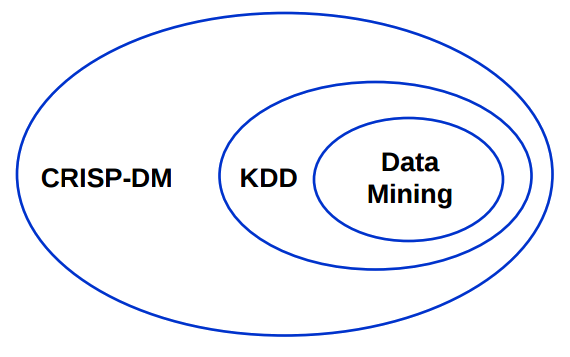
\includegraphics[width=90mm, height=40mm]{Figuras/BigData/RelacaoCrispKddDm.png}\\
\tiny Fonte: Neurotech -- 2012
\end{figure}

\pagebreak

\subsection{Ciclo de vida do CRISP--DM}

O modelo de processo CRISP--DM provê seis fases para um projeto de mineração de dados, sendo assim determina-se um ciclo de vida 
compreendido para cada uma dessas fases:

A figura a seguir ilustra as fases do ciclo:

\begin{figure}[!ht]
\centering
\caption{O padrão CRISP-DM \cite{Crisp2000}}
\vspace{1mm}
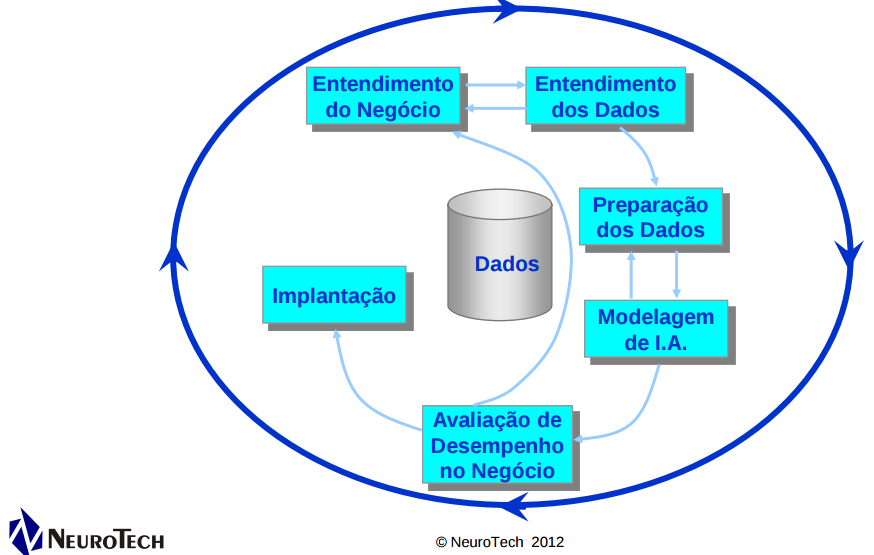
\includegraphics[width=100mm, height=75mm]{Figuras/BigData/CrispDM.png}\\
\tiny Fonte: CRISP-DM 1.0
\end{figure}

A primeira fase, conhecida como \textbf{Entendimento do negócio}, ou ``fase de entendimento dos objetivos e dos requerimentos sob a 
perspectiva do negócio'' (CHAPMAN; KERBER; WIRTH et al, 2000, p.{10}) é uma fase crucial da mineração,  um especialista (ou muitos) deve ser consultado. 
O analista de dados e o analista do negócio traçam os objetivos da mineração sob a perspectiva do cliente. Questionamentos incorretos 
ou negligência nesta fase podem acarretar esforços excessivos no processo como um todo a experiência de um profissional da área 
é condição ``sine qua non'' nessa fase. Portanto avaliar o negócio, avaliar a situação sob o ponto de vista dos riscos de não conclusão 
do processo, determinar os objetivos e traçar um plano para execução. Essas etapas são delineadas nas figuras que se seguem.

\begin{figure}[!ht]
\centering
\caption{Entendimento do negócio}
\vspace{1mm}
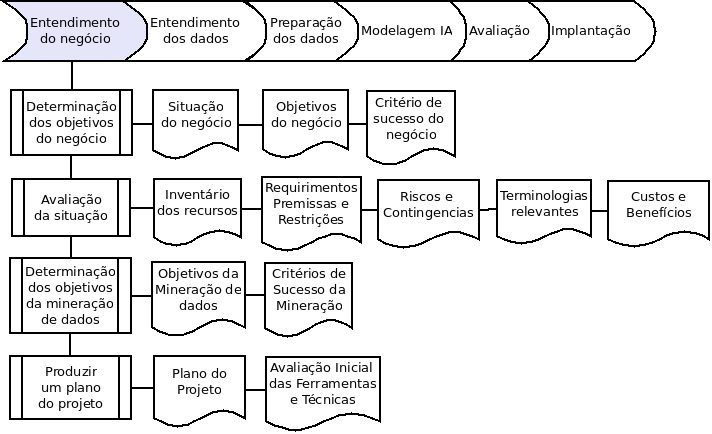
\includegraphics[width=120mm, height=75mm]{Figuras/Cronograma/Entendimento.png}\\
\tiny Fonte: CRISP-DM 1.0
\end{figure}

\pagebreak

\vspace{0.5cm}

Em seguida, o analista de dados passa à segunda fase, \textbf{Entendimento dos dados}. Essa fase caracteriza-se pelo exame acurado dos dados, procurando identificar sua qualidade. 
Dados ausentes -- ``missing data'' -- são comuns em bases de dados não estruturadas, configurando-se como
um problema a ser considerado, pois seu tratamento pode consumir muito tempo do analista de dados, estima-se cerca de 80\% do tempo total. 

\begin{figure}[!ht]
\centering
\caption{Entendimento dos dados}
\vspace{1mm}
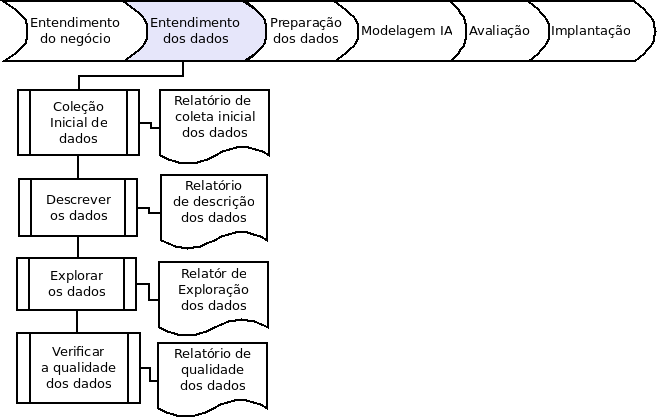
\includegraphics[width=120mm, height=75mm]{Figuras/Cronograma/EntendDados.png}\\
\tiny Fonte: CRISP-DM 1.0
\end{figure}

%\vspace{0.5cm}
\pagebreak


A terceira fase, \textbf{Preparação dos dados}, diz respeito à construção final do conjunto de dados. 
Preparar os dados significa criar e selecionar atributos, criar tabelas ou planilhas e registros dos dados.
Para selecionar quais dados serão mais relevantes, calcula-se, por exemplo, o coeficiente de correlação linear entre os atributos (variáveis), quando as variáveis são numéricas. Outra forma de qualificar os dados é calculando a quantidade de informação que cada atributo possui. A máxima entropia de cada atributo pode fornecer informações sobre a qualidade da variável quando esta estabelece ganho de informação \cite{NorvigRussel2004}, vide equação da Entropia: $ H_{x}=-\sum_{\forall x \in X}P(x)log_{2}P(x) $
Onde $ H_{x} $ é a medida de entropia, x um atributo do conjunto de variáveis $X$ de variáveis. A entropia condicional, formalizada na equação seguinte, é a entropia restante dos atributos de $Y$ no valor $y$ quando o atributo $X$ é dado como $X$ \cite{DecisionTree}:
$ H_{Y|X}= \sum_{x}P(x)H(Y|X=x) =-\sum_{\forall x \in X}P(x) \sum_{\forall y \in Y}P(y|x)log_{2}P(y|x) $ \footnote{Mais adiante será abordado com mais profundidade o conceito de Entropia}.



\begin{figure}[!ht]
\centering
\caption{Preparação dos dados}
\vspace{1mm}
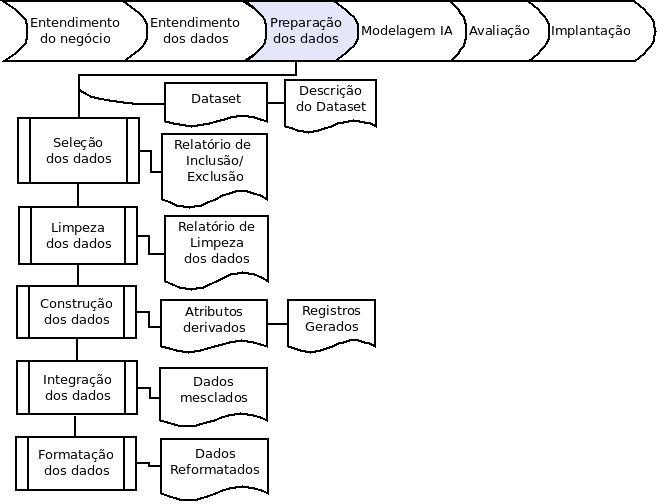
\includegraphics[width=120mm, height=90mm]{Figuras/Cronograma/PreparaDados.png}\\
\tiny Fonte: CRISP-DM 1.0
\end{figure}

\vspace{0.9cm}

Na quarta fase, \textbf{Modelagem de I.A.}, a tecnologia deve ser escolhida de forma criteriosa, baseada na experiência do analista de dados. 
Em sistemas de suporte à decisão, uma tecnologia inadequada pode levar a decisões imprecisas. É comum retornar às fases anteriores para adequar a técnica aos dados. 
Um modelo de regressão logística para problemas binários, redes neurais para problemas de classificação, e assim por diante.

\begin{figure}[!ht]
\centering
\caption{Modelagem IA}
\vspace{1mm}
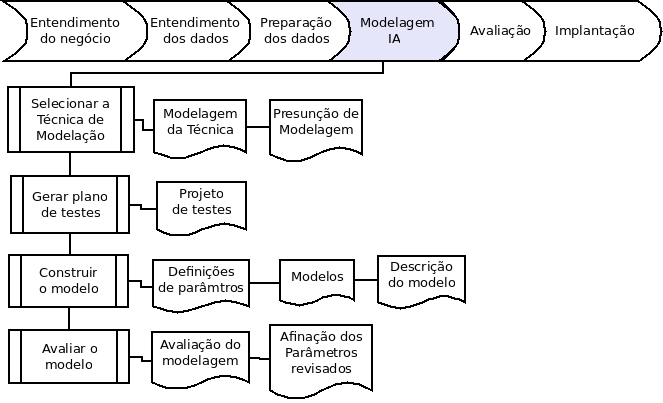
\includegraphics[width=120mm, height=79mm]{Figuras/Cronograma/Model_IA.png}\\
\tiny Fonte: CRISP-DM 1.0
\end{figure}

%\vspace{0.5cm}
\pagebreak

Na fase cinco, \textbf{Avaliação de desempenho}, um ou muitos modelos devem ter sido construídos e testados, 
de forma que seja possível atingir uma alta qualidade do ponto de vista da análise dos dados, ou seja, que o 
modelo proposto esteja de adequado aos objetivos do negócio. Para tal é preciso que antes do desenvolvimento final 
do modelo, os passos executados até então sejam avaliados e revistos.

\begin{figure}[!ht]
\centering
\caption{Avaliação do modelo}
\vspace{1mm}
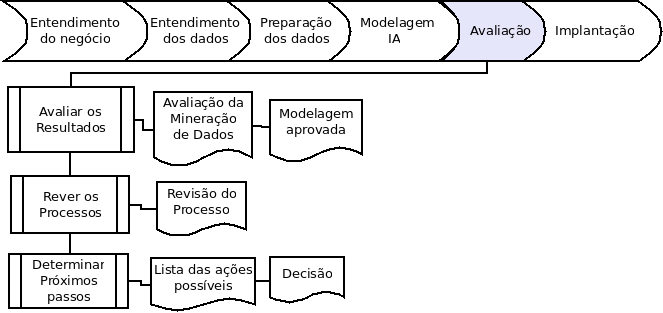
\includegraphics[width=120mm, height=65mm]{Figuras/Cronograma/Avaliacao.png}\\
\tiny Fonte: CRISP-DM 1.0
\end{figure}

\pagebreak

A sexta e última fase, caracteriza-se pela conclusão do modelo. No entanto a criação do modelo não é o fim do processo.
O conhecimento adquirido precisa ser incrementado, organizado e apresentado de maneira que o cliente possa usá-lo.
É importante ressaltar que este ciclo poderá ser retomado até que o modelo esteja adequado às necessidades e especifidades do cliente.

\begin{figure}[!ht]
\centering
\caption{Implantação do modelo}
\vspace{1mm}
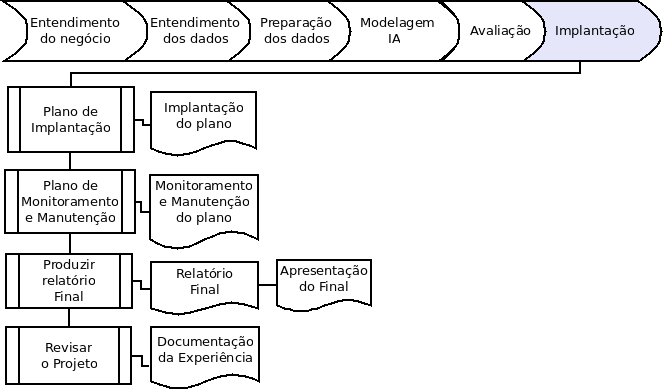
\includegraphics[width=120mm, height=75mm]{Figuras/Cronograma/Implantacao.png}\\
\tiny Fonte: CRISP-DM 1.0
\end{figure}

%\section{Além do KDD -- \textit{Domain-Driven for Data Mining}}

\pagebreak

\section{Mineração de dados}

No processo de extração do conhecimento (KDD), um dos importantes passos a ser considerado é a mineração de dados, que se caracteriza pela aplicação de algoritmos 
específicos para descoberta de padrões e/ou comportamentos em grandes bases de dados, também conhecido como repositórios de dados \cite{FayyadUeoutros}.

A mineração se distingue das técnicas estatísticas pelo fato de que  não trabalha com dados hipotéticos, mas se apoia nos próprios dados para extrair os padrões \cite{CASTANHEIRA, 2008}. 

FAYYAD (1996), destaca que é necessário distinguir claramente KDD e mineração de dados. Enquanto que é um processo, a mineração é um passo no interior desse processo. 
Todavia, esse passo é de considerável relevância para que se possa extrair conhecimento adequadamente. 
A aplicação “cega” dos métodos de mineração de dados, ainda segundo Fayyad \cite{FayyadUeoutros}, pode conduzir à descoberta de dados sem significado e padrões inválidos. 

Existem vários tipos de dados e informações nesses repositórios que podem ser minerados, contudo esses dados, inicialmente são selecionados e agrupados, a seguir passam por 
uma fase de preprocessamento, que consiste em tratá-los de forma a prepará-los para a mineração. Essa fase é de 
fundamental importância na estruturação dos dados, uma vez que em grandes volumes de dados, também conhecido ``Datawarehouse'', podem existir inconsistências, faltas (missing data) ou 
duplicidade e erros de informações.

Nesse sentido, as técnicas de mineração de dados trabalham com dados estruturados, preenchidos em sua totalidade sem \textit{missing data}, para poder extrair informações relevantes.
Existem várias maneiras de se contornar os dados ausentes, como o preenchimento dos dados através de técnicas de inteligência artificial, da média dos valores; quando dados numéricos 
ou com a moda; quando os dados forem categóricos. Para cada tipo de dados existem técnicas apropriadas para serem aplicadas sobre eles, algumas mais sensíveis às problemáticas elencadas anteriormente
e outras mais robustas \cite{DataMining2}, que por sua vez estão associadas a classes de problemas que a mineração trata, a tabela 2.1 delineou o domínio.
Isso será tratado na seção Aprendizagem de Máquina (Machine Learning).
O caminho da extração dos dados até sua mineração e extração de conhecimento é longo.
Na figura a seguir temos a ilustração desse caminho:

\begin{figure}[!ht]
\centering
\caption{Fases da mineração de dados até extração do conhecimento}
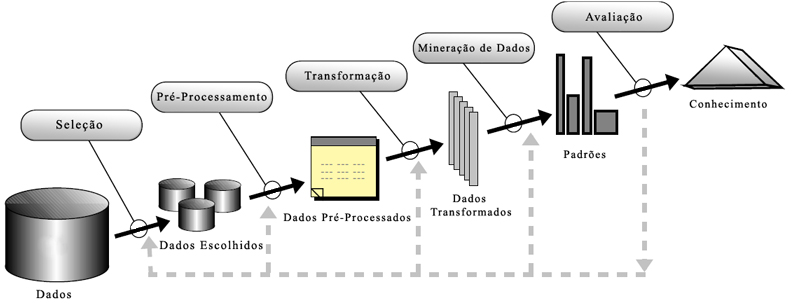
\includegraphics[width=135mm, height=65mm]{Figuras/BigData/Fayyad.png}
\end{figure}


Na origem dos dados, os ``inputs'' estão representados na figura onde se lê ``Dados''. Observa-se que este está repleto de \textit{missing data} e/ou dados inconsistentes, conhecidos como dados não estruturados. 
O balão onde se lê ``Selection'' representa a coleta das informações ou a seleção dos dados no \textit{Big Data}.
Em nossa pesquisa esses dados são provenientes das mais diversas fontes, tais como, redes sociais, câmaras de trânsito, informações de satélites meteorológicos e outras fontes.

Armazenar dados provenientes de redes sociais nessa etapa pode ser um grande problema, devido à sua extensão, porém os dados relevantes podem ser armazenados em ``Target Data'' 
com tecnologia apropriada, utilizando-se técnicas de ``Map'' e ``Reduce'' ou mineração de dados em textos \textit{Text Mining} para criar \textit{cluster} de informações e ler os fluxos de dados (stream data). 
Algumas técnicas de IA podem ser aplicadas nessa etapa como, [``Data Mininng Swarm Robotics'' através de Botnets \footnote{Botnet é citado no sentido da coleta de informações} ou ``Swarm Intelligence''. ]

No balão ``Pré-Processamento'' os dados não-estruturados são tratados, por exemplo, retirando os \textit{missing data}. 
Para estruturar as informações é preciso utilizar técnicas linguísticas, uma vez que existe lógica entre eles \cite{Aranha2006}.
Esses dados normalmente são coletados por técnicas de Mineração de Textos, também conhecidas como Mineração de Dados em Textos, técnicas de IA como ``Machine Learning'' 
têm sido muito utlizadas. Em ``Transformação'' os dados foram em estruturados, podendo ser armazenados em Bancos de Dados, conhecidos como Datawarehouse, por exemplo o Hive. 

O processo de Mineração dos dados começa no balão ``Mineração de Dados'', onde são aplicadas as técnicas de IA conhecidas como classificadores, para extração de padrões, tais como: 
``Decision Tree'' (Árvore de decisão), ``Artificial Neural Network'' (Redes neurais artificiais), ``Logistic Regression'' (Regressão Logística), ``Naïve Bayes'' e ``Deep Learning'', detre outros.
Algumas técnicas de mineração de dados são fortemente influenciadas pelas informações na entrada (input), como as Árvores de decisão \cite{DecisionTree}. 
As Redes Neurais, dependendo da quantidade de variáveis de entrada, paderão ter milhares de neurônios na camada intermediária, o que inviabilizaria essa metaheurística 
\footnote{Metaheurística são heurísticas aplicadas em problemas onde os custos computacionais não são tratáveis em tempo polionomial, devido às explosões combinatórias geradas
pelo grande número de tentativas. Metaheurísticas bioinspiradas metaforizam o comportamento de animais sociais, tais como formigas, pássaros, peixes e outros}.

Todas essas etapas descritas na figura são recorrentes, como indicam as setas pontilhadas que retornam aos passos anteriores.
Utilizar técnicas de mineração de dados, além de extrair dados, extrai conhecimento, com isso pode-se predizer os resultados futuros na saída do modelo, 
quando determinados dados ocorrem na entrada \cite{Amin2015a}, essa técnica de extração de conhecimento chama-se \textit{Knowledge Discovery Databases} (KDD).
O KDD utiliza métodos de Aprendizagem de Máquina para efetuar essa extração.


\pagebreak


\section{Mineração de Textos} %\label{arte:palavraChave:DataMiningBigData}

Minerar dados em texto não é uma tarefa atômica, deve ser divido em várias etapas, minerar em redes sociais é exige ao menos mais uma etapa a escolha da rede social com sua tecnologia própria, então, com processos específicos em cada uma delas e utilizando-se de ferramentas específicas. Extrair conhecimento nos dados não processados não faz sentido, tratá-los apenas ``per si'' exige muito trabalho de IA, como Mineração de dados em textos. A Mineração em textos é inspirada em técnicas de ``Machine Learning'' \cite{Aranha2006}. Todavia, analisar textos é basicamente entender o significado do texto, baseado em regras de associação lógica, como mostrado nos estudos descritos anteriormente. O mapa mental a seguir mostra um modelo de análise de texto feito por seres humanos.

\begin{figure}[htpb]
	\centering
	\caption{Mapa mental da Mineração em textos}
	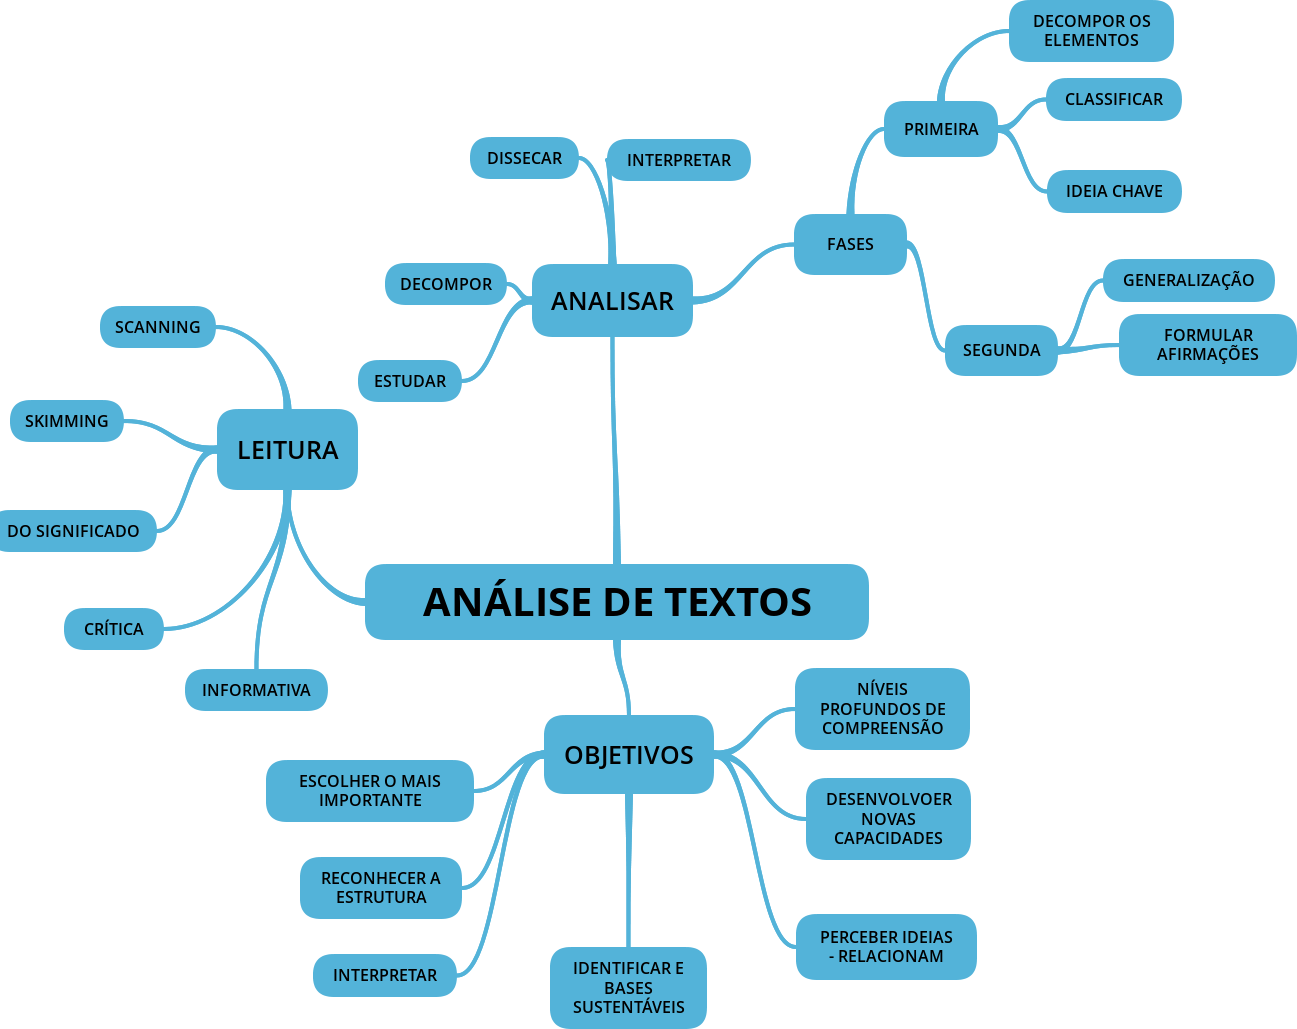
\includegraphics[width=120mm, height=60mm]{Figuras/BigData/Analise_Textos.png}
\end{figure}


\subsection{Mineração de Dados/Textos em Redes sociais}

\subsubsection{Introdução ao estudo das Redes Sociais}

As redes sociais têm assumido, nos dias atuais, um papel essencial na vida de seus usuários. Não apenas como espaço de descontração, mas, sobretudo, como lugar de troca de informações que permitam, dentre outras coisas, tomar conhecimento acerca dos acontecimentos, sejam eles locais ou globais, que influenciarão sua vida. De modo particular, nos grandes centros urbanos, as redes sociais têm servido de fonte de conhecimento acerca de segurança pública, mobilidade urbana e acontecimentos de toda sorte, que possam fazer com que, por exemplo, uma pessoa resolva seguir um ou outro caminho para chegar a um determinado lugar, quer seja ele próximo ou distante de onde se encontre.

Além da troca de informações momentâneas, as redes sociais permitem uma atualização praticamente em tempo real, a partir da utilização de seus usuários e de instituições que também dela fazem uso (por exemplo, a Polícia Rodoviária Federal), de modo que possibilita que decisões sejam tomadas e reorientadas, em virtude da alimentação das informações nas redes.

No que diz respeito às escolhas relacionadas ao trânsito, sejam essas escolhas relativas as áreas urbanas, bem como a centenas de quilômetros adiante, pelo interior de um estado, por exemplo, cada vez mais as pessoas não tomam qualquer decisão sem antes consultar aplicativos e redes sociais tais como o waze, twitter, facebook, ou até mesmo dispõem, em seus aparelhos celulares, de GPS, Google Maps e outras fontes que lhe orientem sobre melhores rotas, que levem com maior rapidez e segurança ao seu destino.

Se pensarmos no transporte de cargas, como tanto já referimos nesse trabalho, a principal função das redes sociais não é de caráter lúdico, mas, sim, como uma ferramenta essencial para que não haja qualquer contratempo que possa causar prejuízo à empresa ou empresas envolvidas, afinal de contas, no que tange ao transporte de mercadorias, sempre há pelo menos duas empresa relacionadas: a de produção do bem e a de transporte do mesmo ao seu destino.

O que discutimos até agora é amplamente sabido por aqueles que analisam o uso das redes sociais na atualidade. O que pretendemos, então, é trazer uma contribuição de natureza científica a essa compreensão e à utilização de forma cada vez mais eficaz dessas ferramentas, a partir do uso da IA, da mineração de dados e dos métodos de extração e produção de conhecimentos (KDD).


"Em 2010 empresas e usuários armazenaram mais de 13 exabytes de novos dados" \cite{bigdataQualquerUm}.

%tabela 5
\begin{table}[!ht]
	\centering
	\caption{Volume de dados no mundo}
	\vspace{1mm}
	\begin{tabular}{l|c|c|c}
		\hline
		\textbf{Ano} & \textbf{Qtd} & \textbf{Unidade} & \textbf{Múltiplo}\\
		\hline
		2000 & 800 & terabytes – TB & $10^{12}$\\
		2006 & 160 & petabytes – PB & $10^{15}$\\
		2009 & 500 & exabytes – EB & $10^{18}$ \\
		2012 & 2,7 & zettabytes – ZB & $10^{21}$\\
		2020 & 35 & yottabytes – YB & $10^{24}$\\
	\end{tabular}
\end{table}

Uma parte desses dados são as redes sociais. A rede social escolhida para esta pesquisa foi o Twitter por apresentar características como API aberta de fácil conexão para obtenção dos dados. Uma rede social é sobretudo uma de conexão entre pessoas, contudo, sob o ponto de vista tecnológico uma conexão entre nós e arestas, os nós simbolizam as pessoas e as arestas a ligação entre elas, essa ``arquitetura social'' é conhecido como grafo. A figura a seguir foi gerada pelo software Gephi \cite{ICWSM09154} representa um grafo da rede social Twitter.

\begin{figure}[!ht]
	\centering
	\caption{Grafo Twitter}
	\vspace{1mm}
	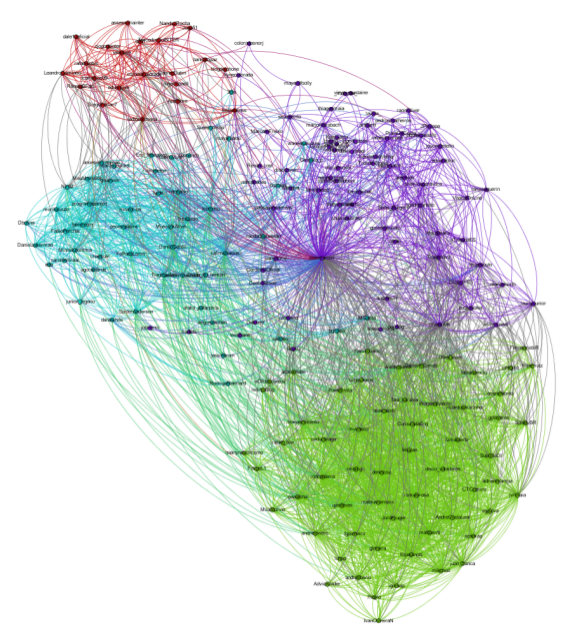
\includegraphics[width=100mm, height=65mm]{Figuras/BigData/grafoExemplo.png}\\
	\tiny Fonte: https://github.com/gephi/gephi/wiki/Official-papers. Acessado em: 10/03/2017
\end{figure}


\pagebreak

\subsubsection{O Twitter}

O Twitter e o Facebook estão entre as mais populares ferramentas de mídias sociais do público em geral. Uma das características-chave
dessas ferramentas é que elas habilitam uma comunicação em dois sentidos e interação entre usuários. A natureza do diálogo tipicamente envolve um tópico específico, muitas vezes relacionados a acontecimentos que têm influência direta na vida das pessoas ou que chamam a sua atenção, como eventos de cunho politico, catástrofes naturais, acidentes com vítimas graves, atentados, dentre outros.

O Twitter, rede social que interessa a essa pesquisa, caracteriza-se como um microblog onde os usuários escrevem em um espaço delimitado (cerca de 140 caracteres) sobre os mais diversos assuntos. Tais usuários conectam o aplicativo por meio de uma multiplicidade de dispositivos: computadores, tablets e celulares, formando uma grande rede social mundial. Essa rede possui duas diferentes APIs, responsáveis pela captura dos dados: Rest API e Streaming API. O Twitter funciona com o padrão de arquivos JSON e os dados são capturados nesse formato. (A FONTE -- BIG SOCIAL DATA: PRINCÍPIOS SOBRE COLETA, TRATAMENTO E ANÁLISE DE DADOS SOCIAIS). A cada dia centenas de terabytes são inseridos no Hadoop data warehouse.

A ideia inicial do Twitter, segundo seus fundadores, era de que essa rede se comportasse como um “SMS da Internet” (30). As informações são enviadas aos usuários, conhecidas como twittes, em tempo real e também enviadas aos usuários seguidores que tenham assinatura para recebê-las: os seguidores. A conexão entre os usuários da rede social se deve à relação entre os seguidores e os seguidos. O comportamento do seguidor para retweetar os usuários seguidos serve como principal mecanismo para compartilhar informações nessas redes.

Nas pesquisas que envolvem as redes sociais, analisar o conteúdo utilizando ferramentas de mineração de textos é um procedimento frequentemente e que tem apontado resultados surpreendentes sobre o comportamento social e suporte à tomada de decisão (Abrahams, Fan, Wang, Zhang \& Jiao, 2015). É comum, ainda, aplicar mineração de textos em bibliotecas e outras instituições. Isso implica em rastrear tópicos, extrair informações, agrupar, categorizar (Fan, Wallace, Rich e Zhang, 2006).

Em recente artigo, Sandhu (2015) indicou a importância do aprendizado sobre mineração de dados e ferramentas de Big Data para as bibliotecas acadêmicas, de forma a melhorar a eficiência da biblioteca e dos serviços de informação. Similarmente, Zhang e Gu (2011) alegaram que minerar conhecimento sobre os clientes é importante para as bibliotecas acadêmicas. Na mesma linha de investigação, Sarker et al., 2015 destacam que a abordagem da mineração de textos para os dados das mídias sociais tem sido utilizada em muitos campos, como negócios, ciência da saúde, dentre outros. 

Estudos atuais têm mostrado o papel da análise sentimental e mineração de opinião nas redes sociais, em particular no Twitter, como forma de investigar padrões de comportamento Twitter as a Corpus for Sentiment Analysis and Opinion Mining Alexander, 2010 Sentiment Analysis on Twitter, Akshi Kumar and Teeja Mary Sebastian, 2012). A figura abaixo mostra como a análise sentimental e a mineração de opinião representam os conhecimentos produzidos nesse tipo de pesquisa.

FIGURA..........

(FONTE: Artigo “Library \& Information Science Research)

Outro estudo (FONTE ??) aponta que em 2013 um número superior a 70\% dos indivíduos adultos que faziam uso da internet estavam conectados a redes sociais. Cerca de 20\% utilizavam o twitter, sendo que aproximadamente 46\% conectando-o diariamente e algo em torno de 29\% mais de uma vez ao dia. (Duggan \& Smith, 2013). Um relatório publicado em 2014 revelou que o Twitter aparecia entre as três maiores mídias sociais, em termos de adesão e utilização, perdendo apenas para o facebook e o youtube (Another Pew). 

Esse relatório revelou, ainda, que naquele ano, nos EUA 8\% dos adultos que tinham entre 18 e 29 anos de idade utilizavam o twitter como principal mídia social. Em outras idades, esse percentual subia para 45\% no mesmo país. As notícias são o principal interesse dos usuários dessa rede (Mitchell \& Page, 2013). Em 2014, os dados revelavam que, em um dia típico, sem qualquer evento extraordinário, essa rede era conectada por cerca de 230 milhões de usuários, responsáveis pela produção de aproximadamente 500 milhões de tweets (postagem tipo microblog) (Twitter, 2014) 

Heneycutt e Hering (2009) identificaram 11 categorias de conteúdo propagados nos tweets: sobre destinatários, anúncio/propaganda, encorajamento “exhort” (que traduzimos aqui como “auto-ajuda”), informações para outros, informações para si próprio, meta comentários, uso de mídia, opinião, outras experiências, auto experiência, e solicitação de informações. Naaman, Boase e Lai (2010), por sua vez, classificaram os conteúdos em oito categorias: Informações compartilhadas, auto promoção, opinião/queixas, declarações e pensamentos aleatórios, eu agora (me now), perguntas aos seguidores, manutenção de presença, e piadas. 

No contexto da Bibliometria e da Cientometria, alguns estudos destacam a utilização da contagem de citações no twitter como o objetivo  de avaliar qual o impacto que uma publicação alcança no público leitor, bem como em centros e instituições de pesquisa (i.e. Adkins \& Budd, 2006, Cronin \& Overflet, 1994; Cunningham \& Dillon, 1997; Lee, 2003). Nos estudos em questão, pesquisadores examinaram a relação entre características dos autores e grupo de autores e o impacto da produtividade deles. Foi medido o número de publicações produzidas e o número de citações recebidas (Haslam et al., 2008; Hinnant et al. 2012; Stivilia et al., 2011). 

Na Web, por sua vez, a quantidade de citações (i.e. links de URL) e estrutura dos links são utilizadas pelos motores de busca (ex: o google) com o objetivo de identificar a relevância e acetiação de wrbsites (Brin \& Page, 1998), em decorrência do número de seguidores, da quantidade de menções feitas, de retweets, por exemplo.

(FONTE: SE É POSITIVO OU NEGATIVO)

Cha, Haddadi e Benevenuto (2010) avaliaram a influência dos usuários no Twitter na rede, como um todo, analisando o número de retweets, menções e seguidores. Esses pesquisadores identificaram uma correlação positiva entre o número de seguidores e o número de retweets pelo top 10 (do Twitter) e o primeiro percentil dos mais conectados, com base no grau do link (i.e. número de seguidores). 

Em outro estudo, André et al. (2012) utilizaram a abordagem “crowdsourcing” para identificar que tipo de tweets chamam atenção e são os preferidos dos seguidores, como também, os que são mais rejeitados. Eles encontraram uma preferência dos usuários em fazer perguntas aos seguidores, bem como em partilhar informações e autopromoção (que diz respeito a algo como falar de si próprio, de seus sentimentos, percepções e ideias).

Modalidades e ferramentas de análise do Twitter 

Nesse tópico abordaremos, em maior detalhe, as escolhas metodológicas e ferramentas analíticas utilizadas em estudos que levam em conta dados do twitter, apresentando alguns dessas pesquisas.
Do ponto de vista metodológico ……….

Na pesquisa conduzida por Suh, Hong e Chi (2010), esses pesquisadores encontraram uma correlação positiva entre a existência de uma URL de um tweet e a probabilidade de que aconteça um retweet. Os autores optaram por uma abordagem indutiva, utilizando-a da seguinte maneira: coletaram 1200 tweets recentes, a partir da conta de uma Universidade, considerando todos os membros da Association of American Universities (AAU). A coleta e processamento dos dados deu-se com a utilização do Twitter API com o twitter4j (biblioteca Java), tendo sido adicionados a um código java desenvolvido pelo autor da pesquisa. Tomou-se uma amostra do percentual da Academia. 

Procederam com o preprocessamento dos dados, de modo a preparar a análise. Nessa etapa, os retweets foram retirados das amostras. Também foram removidos da amostra os tweets com conteúdo pouco significativo para a pesquisa como, por exemplo, breves agradecimentos (e.g. “welcome”), pequenos comentários ou “gírias” de algum tweet (e.g. “lol”), encorajamentos pontuais (e.g. “keep going”) e conversas pessoais, sem relação com o conteúdo dos tweets. Com isto, a amostra foi reduzida de 1200 para 752 tweets que, em seguida, foram distribuídos em nove categorias. Os resultados apontaram que, dos 752 tweets analisados, 271 apresentavam pelo menos um retweet, e 131 receberam um “favorito”.  Em média, tweets recebidos 0,67 (desvio padrão “SD” = 1,4) retweets e 0,23 (SD=0,6) favoritos. Adicionalmente, em média, tweets incluídos 0,47 (SD=0,51) URLs, 0,61 (SD=0,91) menções de usuários e 0,04 (SD=0,2) media de entidades. Em média o tamanho dos tweets foi 107 (SD=29,81) caracteres. 

(REES

Na média, foram enviados, nas seis contas de Twitter das bibliotecas analisadas, cerca de 1817 (SD=1126) tweets, seguido 1062 (SD=641) usuários, estes seguidos por 2006 (SD=788) usuários, e estes 1503 (SD=450) dias (duração). O teste Shapiro-Wilk mostrou que nove característica de tweets normalmente distribuídas. Métodos não paramétricos foram usados para examinar a relação entre um tweet as características da conta. 
O texte Krusal-Walls apresentou uma diferença significativa entre o conteúdo da categoria do tweet para o númro de favoritos $X=15.11, df=8, p<0,057$. O teste Sperman, por sua vez, demonstrou haver uma correlação negativa entre o número de retweets e o número de menções a usuários, sugerindo que tweets com conexões pessoais podem ter pouco valor de ‘uso geral’, de maneira que os usuários demonstram certa relutância em retweetar conteúdos advindos desses seguidores. O teste Spearman encontrou, ainda, uma pequena correlação positiva entre o número de favoritos e o número de usuários seguidos, bem como uma baixa correlação negativa entre o número de favoritos e tempo de uso da conta (desde o cadastro). 

Em outro artigo, conduzido por (FONTE - ANO), os autores justificaram que as mídias sociais têm sido utilizadas cada vez mais para promoção das bibliotecas, com o objetivo de incrementar a relação com os clientes, permitindo “compartilhar informações e conhecimentos, incrementar serviços e promoções, interação com estudantes usuários das bibliotecas, a um custo mínimo” (Chue \& Due, 2013, p. 72). Tal prática têm promovido considerável mudança na interação com usuários e relacionamento com os clientes (Del Bosque, Leif e Skaf, 2012; Cavanagh, 2015), tendo sido utilizada frequentemente como alternativa para estabelecer uma conexão personalizada com os seus usuários (Boaten \& Quan, 2014). 
A pesquisa em questão interessou-se em investigar quantas vezes a biblioteca acadêmica usa o Twitter; tipo de conteúdo compartilhado pela biblioteca acadêmica no twitter; temas associados com os tweets da biblioteca acadêmica. 
(FONTE: Abraham et al., 2015)


(Stieglitz \& Dang-Xuan, 2013)

O corpus de dados desta pesquisa foi obtido a partir da ``timeline'' de dez bibliotecas acadêmicas (i.e. todos Twittes desde a adesão à plataforma), através de um serviço de arquivamento (twimemachine.com), em dezembro de 2014. Foram selecionadas as 10 maiores bibliotecas ranqueadas pelo Shanghai Ranking, tendo a seleção se restringido às universidades de língua inglesa e a apenas uma biblioteca por instituição, para o caso de a universidade ter mais de uma (no artigo original é a tabela 1). As informações relevantes dos tweets, utilizadas para a pesquisa eram: data do tweet; número de vezes em que o tweet foi marcado como favorito por outro usuário; número de vezes em que houve um re-tweet, ou seja, em que ele foi passado para frente; data que se “juntou” ao Twitter.

Na etapa de preprocessamento -- ``dataset prepocessing'' -- o grupo de dados recuperado foi tratado, para reduzir os ``ruídos'', seguindo uma abordagem consistente com outros estudos de mineração em textos, tal como o de Ralston, O'Neil, Wigmore e Harrison (2014) e de Yoon, Elhadad e Bakken (2013). O processo contemplou a aplicação de certo número de filtros. Por exemplo, foram removidas as ``stopwords'', pontuação e numeração, todos os nomes de usuários seguido por um símbolo ``\@'', ``hashtags'' após o símbolo ``\#'' e ``hyperlinks'' após o ``http''. Também foi removido a abreviação do Twitter tal como ``RT'' (retweetes), e ``MT'' (tweet modificado) e palavras tal como ``via''. O nome do usuário do Twitter para cada biblioteca acadêmica também foi excluído. 

Para análise do conjunto de dados, utilizou-se a mineração em textos e para investigar os históricos de tweets da bibliotecas escolheu-se a análise de conteúdo. A frequência dos tweets, retweets e distribuição dos tweets e retweets foi identificada e contabilizada. Em seguida, os tweets marcados com o PamTaT, uma ferramenta ``text mining'' desenvolvida por Pamplin Collage do Instituto Politécnico de Negócios de Virgínia da Universidade Estadual de Virgínia (Poderia colocar essa observação numa nota de 
rodapé). O PamTaT é baseado na interface do Microsoft Excel para Python nltk -- ``natural language processing framework'' (Bird, Loper \& Klien, 2009) e permite a análise de grande volume de textos pelos usuários finais, não necessitando de conhecimento de programação da linguagem Python. 
A ferramenta serve, ainda, para determinar a frequência de palavras simples (unigrams), de duas palavras (bigrams) e sequência de três palavras (trigrams) que aparecem no texto fonte. Com isso, permite desenvolver uma matriz de frequência de termos-tweet, mostrando como sequências de palavras simples e múltiplas palavras (n-grams) são usadas pela biblioteca acadêmica selecionada. Também foi utilizado o Harvard General Inquirer (Stone et al. 1966) para análise semântica e sentimental dos tweets. Essa ferramenta de análise de textos permite ao usuário final repostar a frequência de categorias de palavras diferentes usadas no texto fonte. Aplicações reportadas no ``General Inquirer'' para diferentes textos-fontes identificaram duas centenas de palavras incluindo, dentre elas, palavras que davam o sentido de algo positivo, negativo, ou ainda relacionadas a vontade (prazer), relacionadas a dor, relacionadas a localização, relacionadas a hora (tempo), relacionadas à Academia, relacionadas a exagero (overstatement) ou subavaliação (understatement), e assim por diante. Hurtwitz (2002) forneceu uma lista abrangente de categorias de palavras reconhecidas pela Harvard General Inquirer e apresentou uma lista completa de palavras específicas que pertenciam a cada categoria de palavras. 

Imagem tabela 1 do twitter

Observa-se que foi incluído o número de tweets; a quantidade de usuários seguidos pela biblioteca; a quantidade de seguidores e o número de tweets favoritos da biblioteca. A Universidade Johns Hopkins, como se pode observer na tabela, tem o maior número de
tweets, seguida pela biblioteca da Stanford University e pela biblioteca da Cambrige University, respectivamente. A biblioteca da Universidade da Califórnia San Diego tem a conta do Twitter mais antiga (maio de 2008), mas apresenta um pequeno número de tweets,
comparativamente à biblioteca da Stanford University, que começou no Twitter com uma conta em abril de 2012, mas possui o segundo
maior número de tweets. 

A análise do conteúdo dos Tweets foi desenvolvida da seguinte maneira: tomando a frequência de unigramas (palavras únicas) observou-se (FIGURA), que a palavra mais frequente foi “open”, utilizada em uma variedade de contextos pelos tweets da biblioteca. Por exemplo: foi usada em um anúncio sobre a mudança do horário de funcionamento, bem como EM UM anúncio para abertura do espaço para os estudantes, exposições, abertura da casa (biblioteca), etc. O segundo termo mais frequente foi “research” (pesquisa), que foi utilizado também em diferentes contextos, relacionados frequentemente a apoio, a investigação, por exemplo: workshop research, ferramentas de pesquisa e software, abertura ao acesso para pesquisar, dados e laboratório de pesquisas, guia de pesquisa e ajuda e campos de pesquisa. Outros termos tais como “livros”, “coleções” (acervos) e “on-line” foram utilizados no contexto dos tweets sobre os recursos da biblioteca. Tais termos foram incluidos em tweets relacionados a “e-books”, “textbooks”, “livros raros”, “solicitando e renovando livros”, “comentários de livros”, “novos livros”, “livros de coleções especiais”, “livros recomendados”, “política de circulação de livros”. 

Imagem tabela 2 do twitter

Imagem tabela 3 do twitter

A FIGURA, por sua vez, mostra a distribuição dos bigramas (sequência de duas palavras) no conjunto de tweets. Observa-se que o mais frequente bigrama foi “special collections”.
O segundo mais popular bigrama foi “open access”, utilizado em diferentes contextos, tal como política de acesso, publicidade, recursos, trenamentos e workshops, dicas e orientação, serviços, eventos e notícias. O resultado mostrou a ênfase colocada na iniciativa de promover “open access” com as instituições acadêmicas.

O terceiro maior bigrama foi “reading room”, relativo à atividade de suporte aos estudantes com as instituições acadêmicas. Essas salas são um dos mais importantes espaços da biblioteca, usadas para leitura e estudo. Os tweets eram, em sua maioria, relacionados a noticias de abertura e fechamento das salas de leitura: “reading rooms”.

A fig-6 mostra os mais importantes trigramas (sequência de três palavras), dos quais destacou-se o trigrama “save the date”. Essa expressão era utilizada para requerer especial atenção dos seguidores para os eventos importantes que estavam para acontecer. Este trigrama é seguido, como o segundo mais frequente, por “pleased to announce”, outra expressão usada para enfatizar a importância de eventos especiais. O terceiro mais usado foi “open access week” (seguido muito próximo por “open access policy”), que novamente destaca os esforços na iniciativa de espaço aberto (open access) 

Imagem tabela 4 do twitter


No caso particular dessa pesquisa, o interesse voltou-se para os tweets da Polícia Rodoviária Federal do estado de Pernambuco, bem como de seus seguidores e de usuários que fizeram menção a eventos que afetam diretamente o tráfego nas principais rodovias do estado. A seguir, a título de exemplo, pode-se verificar uma sequência de twittes da Polícia Rodoviária Federal do estado de Santa Catarina:

\begin{figure}[ht]
	\subfigure{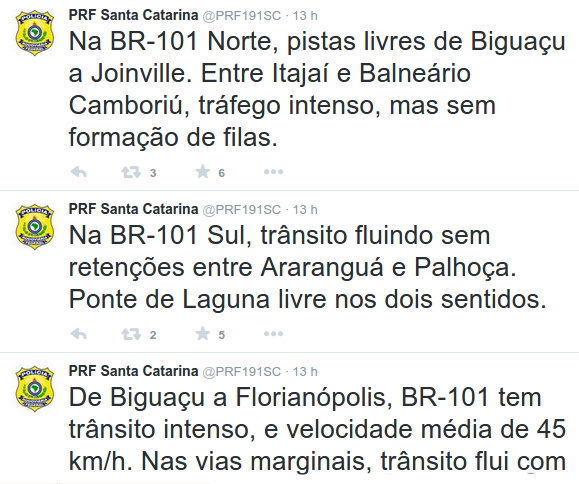
\includegraphics[width=60mm, height=48mm]{Figuras/BigData/twittePRF.png}}
	\quad \quad \quad \quad
	\subfigure{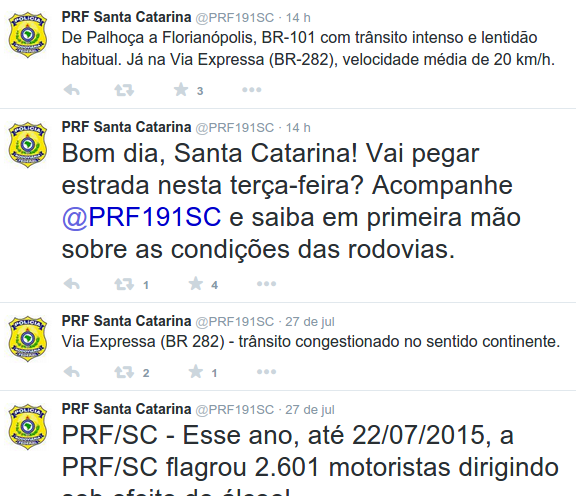
\includegraphics[width=60mm, height=48mm]{Figuras/BigData/twittePRF2.png}}
\end{figure}

A Polícia Rodoviária Federal disponibilizou às 13h através do canal @PRF191SC, informações relevantes sobre o trânsito naquela localidade, 
num espaço temporal variado. Por exemplo: entre Itajaí e Balneário Camboriú foi informado que o trânsito estava intenso, sugerindo que a frota de caminhões deva ter uma rota alternativa, caso a situação persista por muito tempo. No primeiro twitte da segunda coluna, é informado em Via Expressa (BR 282) que o trânsito está lento com velocidade de 20km/h (praticamente congestionado). 

\pagebreak

Outra rede social conhecida pelos condutores de veículos é o Waze. O Waze é um aplicativo de navegação para o trânsito, e funciona em aparelhos celulares e tablets. Os utilizadores desse aplicativo são conhecidos como wazers e compartilham informações sobre o trânsito, em tempo real. Todavia, as informações somente estão disponíveis no momento em que são postadas pelos utilizadores, por um período de tempo pequeno. Caso não haja usuários trafegando pelas vias, ou caso os mesmos não tenham disponibilidade para compartilhar informações, não há o que se ver. Outro problema lidentificado em relação ao waze é que caso não haja conexão à Internet, não há como acessar os dados dos 'wazers', para navegação.

Além dos dados que chegam ao \textit{Big Data} através das redes sociais, as grandes cidades têm disponíveis câmeras de monitoramento do trânsito nos semáforos ou próximas a eles. Algumas com cobertura por canais de televisão, bem como câmaras de segurança próximas às rodovias, coletando informações em tempo real. Os dados desses dispositivos são gravados, sendo conhecidos como \textit{stream} de dados. Esses \textit{streams} podem ser disponibilizados na Internet, em sítios eletrônicos especialmente construídos para isso, como o http://vejoaovivo.com.br (acessado em 10/10/2016) dentre outros.

Os dados disponibilizados pelos diversos meios de comunicação não estão em formato que possam ser utilizados imediatamente, precisando antes serem processados. Tais dados não processados são conhecidos como ``dados frios''. O processo de tratar as informações, retirando-lhes o ``lixo'' e transformando dados ``frios'' em dados ``quentes'', é um processo que tem um custo temporal elevado, devido ao volume dos dados.


\section{Aprendizagem de Máquina} \label{arte:palavraChave:Machine}

Historicamente, a aprendizagem computacional está relacionada com ``o que'' há para ser aprendido \cite{Nilsson2005}. 
Para escolher o que aprender é necessário definir de ``onde'' ou sobre quais dados aprender.
Deve ser fornecido um conjunto de treinamento, para, em seguida, testar o conhecimento aprendido em um ``conjunto de teste''.

Aprendizagem de Máquina ou ``Machine Learning'' são métodos para analisar dados de forma automatizada e interativa.
Segundo Shalev-Shwartz \& Ben-David \cite{Ben-David2014}, o termo Aprendizagem de Máquina refere-se à detecção automatizada de Padrões de dados.

Para Nilsson \cite{Nilsson2005}, o aprendizado ocorre quando uma máquina modifica sua estrutura interna, programa ou dados 
(baseados nos inputs ou em uma resposta para informação externa) de tal maneira que melhora o desempenho futuro. Por exemplo, quando uma máquina de reconhecimento da fala melhora após ``ouvir'' várias amostras de fala humanas e que nós sentimos que pronta, neste caso podemos dizer que a máquina aprendeu. 

Sistemas que executam tarefas de inteligência artificial, tais como Reconhecimento de Padrões, Diagnóstico, Controle de Robôs, Predição e outros, precisam ser modificados para executarem ``Machine Learning'' \cite{Nilsson2005}.


\subsection{Tipos de Aprendizagem}

Quando se fala em algoritmos de IA, adentramos no campo de Aprendizagens e Máquinas. É o princípio da aprensizagem que faz com que o algoritmo estabeleça a decisão adequada para o problema proposto.
No campo da aprendizagem de máquina, é possível apontar três tipos de aprendizagem: a aprendizagem supervisionada, aprendizagem não-supervisionada e aprendizagem por reforço \cite{NorvigRussel2004}. AS duas primeiras serão aqui descritas de maneira sucinta, e consideradas mais adiante, uma vez que interessam particularmente a essa pesquisa, sobretudo quando da utilização de redes neurais e árvores de decisão. 

A aprendizagem supervisionada \cite{Monard} se caracteriza pelo acesso ao conjunto de exemplos de treinamento pelo algoritmo de aprendizagem, também conhecido como indutor, de modo que haja especificação da saída desejada.
No caso da aprendizagem não-supervisionada (RUSSEL; NORVIG, 2004), os valores de entrada são estabelecidos, mas não são definidos os valores de saída. O indutor terá o papel de estabelecer aproximações, propondo agrupamentos (clusters) em função de determinadas categorias como, por exemplo, similaridade \cite{Monard}.

Para ``aprender'' sobre uma determinada função \textit{f} definimos uma amostra em um conjunto de treinamento $X = {x_{1}, x_{2}, ...x_{n}}$.

As técnicas algorítmicas apresentadas nas seções subsequentes são parte da grande família de algorítimos que compõem 
o aprendizado de máquina aplicado a mineração de dados.

A descoberta de conhecimento através da aplicação das técnicas de mineração de dados podem ser agrupadas de acordo com suas funcionalidades \cite{DataMining2}, 
essas funcionalidades tem como característica principal a maneira como são descobertos os padrões no dados, elas podem estar 
em uma das duas categorias: tarefas descritivas ou tarefas preditivas. As tarefas mineração descritivas preocupam-se nas características 
dos dados no conjunto de dados; o ``data set''. As tarefas de mineração preditivas induzem regras nos dados correntes para produzirem 
predições \cite{DataMining2}. A seção seguinte analisa as tarefas preditivas.



\section{Algoritmos de Aprendizagem de Máquina}

\subsection{Naïve Bayes}

Naïve Bayes é uma classe de algoritmos baseado no teorema da probabilidade condicional de Bayes, serve para rotular classes de variáveis independentes. Em mineração de dados variáveis independentes explicam a variável dependente para fazer predição. Este classificador tem sido muito empregado para classificar documentos e detectar spam em mensagens \cite{bibid}. A probabilidade condicional pode ser explicada por um vetor $x = (x_{1}, x{2}, ..., x{n})$ que se representa \textit{n} características (variáveis independentes) que se atribui a estas instâncias de probabilidades $p(C_{k}|x_{i},...,x_[n])$ para cada \textit{K} possível ter vindo da classe $C_[k]$. Aplicando o teorema de Bayes da probabilidade condicional temos:

\begin{equation}
p(C_{k}|x) = \frac{p(_{k})p(x|C_{k})}{p(x)}
\end{equation}

Em outras palavras, a medida que se conhece os resultados das probabilidades pode-se predizer os novos resultados porque o conjunto de testes torna-se menor. A probabilidade condicional também pode ser entendida como:

\begin{equation}
p(posteriori) = \frac{p(priori) * verossimilhança}{evidência}
\end{equation}


\subsubsection{Aprendizagem Bayesiana}

Baseado no teorema de Bayes, dado um conjunto de variáveis aleatórias $\omega = {x_{1}, x_{2},..,x_{n}}$ a variável aleatória \textit{H} (hipótese) denota o tipo de $\omega$, com valores possíveis para $h_{1}, h{2},...,h_{n}$. A medida que são inspecionadas as variáveis, são revelados os dados $D_{1}, D_{2},...,D_{n}$, onde $D_{i}$ é uma variável aleatória com valores possíveis para cada variável do conjunto $\omega$ de variáveis. Sendo D a representação dos dados do espaço de variáveis para uma predição sobre a parte deconhecida de \textit{X}, temos:

\begin{equation}
P(h_{i}|d) = \sum_{i}P(X|d,h_{i})P(h_{i}|d) = \sum_{i}P(X|h_{i})P(h_{i}|d)
\end{equation}
 onde cada hipótese $h_{i}$ determina uma distribuição de probabilidades sobre a variável \textit{X} \cite{NorvigRussel2004}.




\pagebreak

\subsection{Árvores de Decisão}

\subsubsection{Aspectos introdutórios}

No âmbito da inteligência artificial, quando se trata de algoritmos de aprendizagem, uma classe de algoritmos que tem se revelado potente para problemas das mais diversas naturezas é a árvore de decisão. Além do universo das pesquisas no campo da informática engenharia e ciências da computação, as árvores de decisão têm sido utilizadas, sobremaneira, em pesquisas relacionadas à Medicina, à Economia, nos mais diversos sistemas de suporte à decisão, como diagnósticos de doenças, investigação de fraudes, dentre outros \cite{Camilo}.

A escolha desse algoritmo está relacionada, em larga medida, a uma relação que cotidianamente chamamos de “custo benefício”. Uma árvore de decisão é gerada de maneira relativamente simples e os resultados produzidos são, em sua maioria - e a depender da área específica – de grande poder de abrangência e de fácil interpretação. Todavia, para que se faça opção por essa ferramenta, o pesquisador precisa ter clareza sobre a que classe de problemas ela atende, bem como, de que maneira pode ser gerada e realimentada, e de que forma seus resultados devem ser adequadamente interpretados.

Na pesquisa apresentada nessa dissertação, particularmente, as árvores de decisão possibilitaram grandes avanços na proposição do modelo de predição, conforme pode ser observado no capítulo dedicado aos resultados. 

Conforme o nome sugere, o que se espera de uma árvore de decisão é que ao final do processo resulte a melhor decisão. Todavia, para que a decisão satisfatória apareça, é necessário que o pesquisador faça as escolhas adequadas, de modo a poder tirar o melhor proveito dessa ferramenta. Para tal, é preciso compreender a natureza desse algoritmo e os processos a ele relacionados. A seguir serão apresentados os principais elementos que precisam ser conhecidos pelo pesquisador que deseja se aventurar por esse campo.

\subsubsection{Breve histórico e conceituação}

De maneira sintética, uma árvore de decisão tem como entrada um conjunto de atributos e como saída uma decisão. Os atributos podem, ainda, ser classificados de duas maneiras: discretos ou contínuos. Em virtude dos atributos de entrada, tem-se, como resultado uma função de valores discretos – aprendizagem de classificação – ou de valores contínuos – aprendizagem de regressão \cite{NorvigRussel2004}.

A decisão gerada aparece em função de uma sequência de testes executados, estando cada um deles relacionados a um nó da árvore. As ramificações que decorrem dos testes são o resultado encontrado a partir da realização do experimento. 
O exemplo a seguir ilustra uma árvore de decisão simples, onde se vê seu nó-raiz e suas ramificações. 

\begin{figure}[!ht]
	\centering
	\caption{Árvore de decisão}
	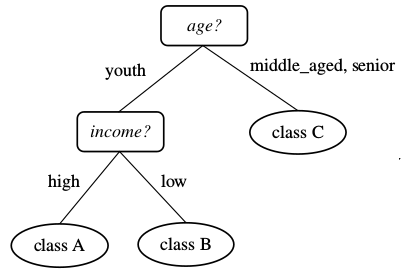
\includegraphics[width=60mm, height=45mm]{Figuras/Arvore/arvorejovem.png}\\
	\tiny Fonte: Han, J. and Kamber, M. 
\end{figure} 


Uma árvore de decisão obedece à regra básica “se-então”, de maneira que, parte-se do nó (se) até as folhas (então). O conhecimento é representado em cada nó, que apresenta pelo menos duas saídas ou ramificações possíveis, que pode, ou não, converter-se em um novo nó, relacionado a um novo nível. 

Embora seja um algoritmo simples e de fácil interpretação, uma das mais importantes questões a ser considerada é como propor as regras de forma adequada e relevante para a geração da árvore. É necessário identificar o melhor atributo, que será  responsável por criar o nó de decisão. As ligações entre os nós representam os valores possíveis do teste do nó superior e as folhas indicam à classe (categoria) a qual o registro pertence \cite{Camilo}.

A origem das árvores de decisão, como algoritmo no campo da inteligência artificial data da segunda metade do século XX. A literatura aponta que as árvores de decisão foram propostas por Ross Quinlan, pesquisador australiano, no final da década de 70 e início dos anos 80, sendo o ano de 1983 aquele em que foi apresentado o primeiro algoritmo para geração de árvores de decisão: o ID3 (Iterative Dichotomiser),  utilizado até hoje e considerado um dos mais importantes.  

Todavia, HSSINA; MERBOUHA; MOHAMMED \cite{Decision2014}, sugerem que autores no campo da estatística descrevem que seu surgimento na deu década de 60, com Sonquist e Morgan, que utilizaram árvores de decisão para predição e explicação, com o algorítmo AID (Automatic Interation Detection), sem tomar conhecimento das pesquisas de Quinlan. A partir desse modelo, houve uma expansão para problemas de classificação e discriminação, cuja abordagem teria culminado no CART (Classification and Regression Tree), método desenvolvido por Breiman e seus colaboradores.

Quinlan \cite{Quinlan86inductionof} discute que desde que a inteligência artificial começou a se desenvolver como campo de teorização e investigação, em meados dos anos 50, as máquinas de aprendizagem (machine learning) ocuparam um lugar de particular interesse dos pesquisadores, sobretudo pela na compreensão e modelização de comportamentos inteligentes. 

Tal interesse, ainda segundo esse autor, instigou a busca pelo desenvolvimento de sistemas competentes baseados no conhecimento (knowledge-based) e tomou vulto nas pesquisas em inteligência artificial. Quinlan \cite{Quinlan86inductionof} avança, pontuando o interesse de muitos pesquisadores, dos quais ele próprio, no que ele chamou de “microcosmo de máquinas de aprendizagem e de uma família de sistemas de aprendizagem que têm sido utilizadas para construir sistemas baseados em conhecimentos de um tipo simples” ( p.82) (livre tradução do autor). \footnote{This paper focusses on one microcosm of machine learning and on a family of learning systems that have been used to build knowledge-based systems of a simple kind.}

O primeiro grupo de árvores de decisão, ainda conforme Quinlan \cite{Quinlan86inductionof} era responsável por tarefas de classificação, desenvolvendo uma decisão das raízes às folhas, sendo conhecido com \textit{Top -- Down}. 
\footnote{ Em uma árvore de decisão, embora seu desenvolvimento se dê das raízes às folhas, a sua representação começa pelo nó-raiz, na parte superior, descendo em direção às folhas.} O modelo proposto comportaria – como o é até hoje – inúmeras análises e reanálises, em todos os estágios e durante todo o processo. Assim, esse primeiro modelo faria parte da família de algoritmos do tipo Top-Down Induction of Decision Tree – TDIDT, representada por Quinlan, em forma de árvore, na figura a seguir (p. 84).

\begin{figure}[!ht]
	\centering
	\caption{Árvore da família TDIDT}
	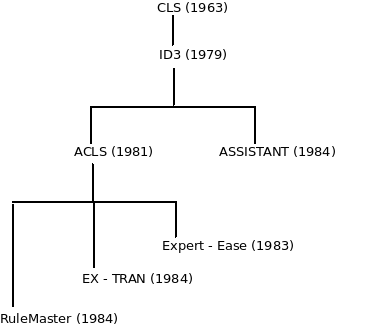
\includegraphics[width=60mm, height=45mm]{Figuras/Arvore/TDIDT.png}\\
	\tiny Fonte: J. R. Quinlan. 
\end{figure} 

Para Quinlan \cite{Quinlan86inductionof}, o pai da família TDIDT é o Sistema de Aprendizagem de Conceito (Concept Learning System – CLS) de Hunt, proposto em 1963, que constrói uma árvore de decisão que visa diminuir o custo de classificar um objeto. Para cada etapa o CLS explora o conjunto de decisões possíveis, seleciona uma ação que minimize o custo, para então mover a um nível abaixo na árvore. O ID3 configura-se, então, como um entre uma série de programas desenvolvidos em função desse Sistema (CLS).

O ACLS \cite{Quinlan86inductionof}, por sua vez, seria uma generalização do ID3. Enquanto que o CLS e o ID3 têm propriedades que possibilitam descrever objetos apenas com valores de um grupo especifico, o ACLS permite propriedades com valores não restritos, podendo ser aplicado para tarefas das mais complexas, tal como o reconhecimento de imagens.

O “Assistant” (ver figura anterior), por sua vez, generaliza atributos do ACLS, permitindo atributos valores contínuos. E, embora não produza uma árvore de decisão iterativa, como acontece com o ID3, tem o poder de escolher um conjunto de treinamento para os objetos disponíveis. Essa classe de algoritmos tem sido bastante utilizada no campo médico, por exemplo.


Ainda na figura anterior, os três sistemas à esquerda são derivações comerciais do ACLS, que não estão relacionados a avanços teóricos consideráveis, mas incorporam inovações simples e de sucesso na geração e utilização de árvores de decisão.

Conforme mencionado, a tarefa das árvores de decisão desse tipo é a de classificação.  Seu produto será, pois, uma classe. Para tal, \cite{Quinlan86inductionof} descreve que a estratégia subjacente a essa árvore é não-incremental, ou seja, um grupo de casos relevantes é apresentado, os exemplos são dados, mas não há uma ordem específica de apresentação dos mesmos. 

Ainda do ponto de vista histórico, no final da década de 80 e início da década de 90 \cite{Kohavi99decisiontree} é desenvolvido o algoritmo C4.5, uma evolução significativa do ID3, que consegue lidar tanto com atributos categóricos, quanto contínuos. É também capaz de lidar com valores desconhecidos, representados por “?” e sendo tratados de forma especial no processo.

No W.E.K.A. (Waikato Environment Knowledge Analysis) é disponibilizada sua implementação, passando a ser chamado J48, que é a implementação na linguagem Java do algoritmo utilizado na pesquisa contemplada nessa dissertação.

O C4.5 é capaz de analisar a medida de ganho, introduzindo um conceito fundamental para o avanço desse algoritmo: a “poda”, que é realizada utilizando medidas estatísticas para identificar e, posteriormente, excluir ramos. Tal processo permite o recorte de ramos que não apresentam contribuição significativa, melhorando o desempenho do algoritmos, que se tornou um dos  mais utilizados na literatura que contempla árvores de decisão. 

São identificadas dois momentos em que são realizadas as podas. O primeiro é o de pré-poda, efetivado no treinamento e que se caracteriza pela interrupção do processo de divisão do nó “em função da avaliação de um conjunto de medidas, transformando o nó em folha rotulada com a classe majoritária” \cite{Simoes2008}. A pós-poda, por sua vez, é executada findo o processo de construção da árvore, e é aplicada recursivamente, na direção de baixo para cima.

Segundo Quinlan \cite{Kohavi99decisiontree}, os dados de entrada do C4.5 são caracterizados por uma coleção de casos de treinamento, cada uma com um tupla de valores para um grupo de atributos (variáveis independentes) e uma classe de atributos (variáveis dependentes). Um atributo, por sua vez, pode ser contínuo ou discreto.

Para Ian e Frank \cite{MachineLearning}, as árvores de decisão geradas a partir do C4.5 podem ser representadas por uma abordagem ``dividir para conquistar'' para resolução de problemas de 
aprendizagem, a partir de um conjunto de instâncias independentes. Os nós em uma árvore de decisão ``testam'' um atributo específico, comparando seu valor com uma constante. No entanto, algumas árvores podem comparar dois atributos com outros ou utilizarem uma função para tal.

O último algoritmo de árvores de decisão que pretendemos contemplar nessa breve revisão histórica é o CART – Classification and Regression Trees \cite{breiman1984}. Esse algoritmo produz tanto árvores de classificação (para o caso de atributos discretos) quanto de regressão (para atributos contínuos). 

O CART é conhecido, sobretudo, pela técnica de partição recursiva binária, tendo em vista que cada nó é dividido em dois outros nós, que podem ser divididos, cada um, em mais dois nós, sucessiva e recursivamente. É estabelecido um conjunto de regras que dão suporte à divisão de cada nó, até a decisão de que a árvore está completa.

Diferentemente do C4.5, o CART não realiza pré-poda. A poda acontece ao final – pós-poda - da árvore gerada, em seu tamanho máximo, e por meio da relação custo-complexidade \cite{breiman1984}, obtendo, muitas vezes, subárvores, que são analisadas e, via de regra, a melhor delas é escolhida.
Ainda no que diz respeito ao CART, o critério de classificação utilizado é o índice de Gini. Esse índice tem como base o cálculo da entropia, e é utilizado frequentemente como parâmetro de pesquisa no campo sócio-econômico.

\subsubsection{Conceito de Entropia}

A entropia é um conceito, utilizado na química e na física, para medir a quantidade de desorganização da matéria. WIENER e SHANON \cite{Pineda2006} lançaram mão desse conceito para analisar a desorganização da informação. Quando há alta entropia, pode-se dizer que a informação está com nível considerável de desorganização ou de medida de incerteza.

No caso das árvores de decisão, a entropia aparece relacionada ao ganho de informação. Quando um atributo é identificado como aquele que está relacionado a um maior ganho de informação (ou maior redução de entropia), ele é escolhido como o atributo teste para o nó. Tal atributo teria, então, a função de diminuir a aleatoriedade ou impureza nas partições \cite{Simoes2008}. Com essa abordagem é possível reduzir o número de testes necessários para que uma árvore seja produzida.

(CONTINUA)


\pagebreak

\subsection{Redes Neurais}

\subsubsection{Introdução}

O cérebro humano possui cerca de 10 bilhões de neurônios, que são responsáveis pelo funcionamento do organismo. 
Esses neurônios se conectam entre si, através de sinapses, formando uma Rede Neural capaz de armazenar e processar grande quantidade de informações.

De forma semelhante ao funcionamento das Redes Neurais naturais, foram desenvolvidas as Redes Neurais Artificiais, que recebem esse nome por se caracterizarem como um 
sistema cujo funcionamento é semelhante à arquitetura das redes neurais humanas.

Nesse contexto, em que se pretende criar modelos computacionais com funcionamento semelhante ao modelo neurológico humano, surge a chamada neurocomputação. 
No início da década de 40, precisamente em 1943, McCulloch e Pitts \cite{Heaton2008} propuseram um modelo simplificado de funcionamento do cérebro humano e, 
a partir dai sugeriram a construção de uma máquina que fosse inspirada nesse funcionamento.

A partir da proposição de McCulloch e Pitts, vários trabalhos começaram a ser desenvolvidos, tomando o funcionamento do cérebro humano como modelo. 

Em 1949 Hebb explicitou matematicamente as sinapses dos neurônios humanos. Dois anos depois, em 1951, o primeiro neurocomputador, 
chamado Snark, foi desenvolvido por Mavin Minsky. Todavia, o primeiro neurocomputador que obteve sucesso surgiu entre 1957 e 1958, 
o Mark I Perceptron, criado por Rosenblatt, Wightman e colaboradores \cite{Heaton2008}. O interesse principal desses pesquisadores era o de desenvolver, com esse neurocomputador, a capacidade de reconhecimento de padrões. Nesse contexto, os estudos na área se aprofundaram de tal forma, que muitos consideram Rosenblatt como o fundador da neurocomputação, tal qual encontramos hoje. 

A figura a seguir ilustra, de maneira simplificada, a Rede de Perceptrons, conforme proposta de Rosenblatt.

\begin{figure}[!ht]
\centering
\caption{Percepton de Rosenblatt}
\vspace{1mm}
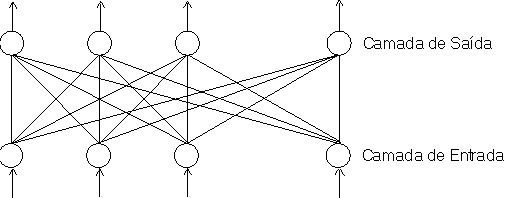
\includegraphics[width=90mm, height=30mm]{Figuras/Neural/Rosenblatt.png}\\
\tiny Fonte: http://www.din.uem.br/ia/neurais/neural. Acessado em: 01/10/2016
\end{figure}


Dando continuidade e indo mais além dos trabalhos de Rosenblatt e seus colaboradores, Widrow desenvolveu, em conjunto com alguns 
alunos, o Adaline, um tipo de processamento de redes neurais dotado de uma potente lei de aprendizado, em uso ainda nos dias atuais, 
que pode ser representado pela figura abaixo:

\begin{figure}[!ht]
\centering
\caption{Rede ADALINE e MADALINE}
\vspace{1mm}
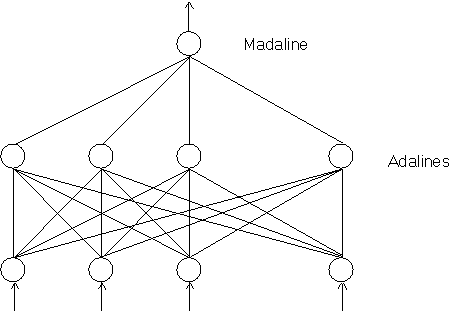
\includegraphics[width=85mm, height=40mm]{Figuras/Neural/Adaline.png}\\
\tiny Fonte: http://www.din.uem.br/ia/neurais/neural. Acessado em: 01/10/2016
\end{figure}

\pagebreak

Muitos estudos foram realizados nas décadas seguintes, mas o que marcou esse período foram as elucubrações sobre o 
desenvolvimento de máquinas tão potentes quanto o cérebro humano, muito mais do que a publicação de pesquisas realmente 
contundentes na área.

A partir dos anos 80, a pesquisa em neurocomputação deu outro grande salto qualitativo e em 1987 teve lugar, em São Francisco a 
primeira conferência de redes neurais nos tempos modernos: a IEEE International Conference on Neural Networks, sendo também formada 
a International Conference on Neural Networks Society (INNS). 
Em 1989 foi fundado o INNS Journal, e em 1990 o Neural Computation e IEEE Transations on Neural Networks.

\subsubsection{Definições e funcionamento de uma Rede Neural Artificial}

São várias as definições que podem ser encontradas sobre o que vem a ser uma Rede Neural Artificial (RNA) \cite{Castanheira}, em função da complexidade de tal Rede. 
Do ponto de vista computacional, uma RNA configura-se como uma técnica para solucionar problemas de Inteligência Artificial (IA) que estabelece um modelo matemático 
baseado em funções de um modelo neural biológico simplificado, com capacidade de aprendizado, generalização, associação e abstração.

Uma grande rede neural artificial pode ter centenas ou milhares de unidades de processamento, enquanto que o cérebro de um mamífero pode ter muitos bilhões de neurônios. 
Uma Rede Neural Artificial (RNA) é um sistema que de neurônios que estabelecem conexões sinápticas, que possuem neurônios de entrada, que recebem os estímulos provenientes 
do meio exterior, os neurônios internos ou hidden (neurônios ocultos) e os neurônios de saída, que se comunicam com o mundo externo \cite{Tatibana}.

Cabe destacar que, de acordo com esse modelo, os neurônios internos têm considerável importância nesse processo, uma vez que são responsáveis pela resolução de problemas linearmente inseparáveis. 
O comportamento inteligente de uma Rede Neural Artificial vem das interações entre as unidades de processamento da rede.

Os neurônios, nessas redes são conhecidos como Perceptrons. O arranjo em camadas desses perceptrons é chamado \textit{Multilayer Perceptron}.
O \textit{multilayer perceptron} é responsável pela resolução de problemas mais complexos que não seriam passíveis de resolução pelo modelo 
de neurônio básico. Para aprender os perceptrons tem que estar dispostos em camadas, um único perceptron pode realizar algumas operações do 
tipo XOR, contudo seria incapaz de aprendê-la.

A figura a seguir apresenta o arranjo dos perceptrons em camadas, conforme discutido anteriormente.
\pagebreak

\begin{figure}[!ht]
\centering
\caption{Um arranjo de Perceptrons em camadas}
\vspace{1mm}
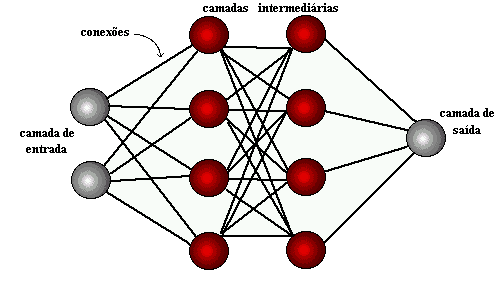
\includegraphics[width=90mm, height=50mm]{Figuras/Neural/camdasIntermediarias.png}\\
\tiny Fonte: http://www.din.uem.br/ia/neurais/neural. Acessado em: 01/10/2016
\end{figure}

São três as camadas usualmente identificadas em uma rede de perceptrons:
\begin{itemize}
 \item Camada de entrada: nessa camada apresenta-se os padrões à rede;
 \item Camadas Intermediárias (ocultas): aqui é realizada a maior parte do processamento por conexões ponderadas. São consideradas como as camadas 
 extratoras de características;
 \item Camada de saída: responsável pela conclusão e apresentação do resultado.
\end{itemize}

O comportamento inteligente de uma Rede Neural Artificial vem das múltiplas interações existentes entre as unidades de processamento dessa rede. 
As unidades de processamento são conectadas por canais de comunicação, associados a determinado peso, como mostra a figura a seguir, proposta por McCulloch e Pitts (1943)

\begin{figure}[!ht]
\centering
\caption{Perceptron de McCulloch e Pitts}
\vspace{1mm}
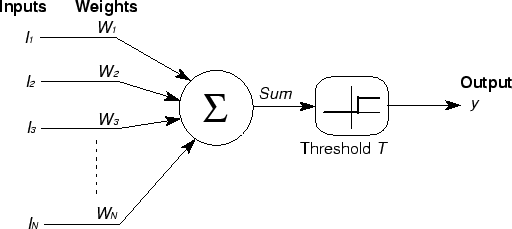
\includegraphics[width=90mm, height=40mm]{Figuras/Neural/Perceptron.png}\\
\tiny Fonte: http://www.din.uem.br/ia/neurais/neural. Acessado em: 01/10/2016
\end{figure}

Esses canais são os  \textit{inputs}, $ I_{1}, I_{2}, I_{3},...,I_{n}$, e cada um tem um peso associado, que serão calibrados de acordo 
com a aproximação do resultado esperado pela rede neural, produzido na saída (fase de ``forward''). 
Essa aproximação é conhecida como erro ou erro padrão. Esse erro será propagado de volta à entrada, retroalimentando a rede neural (fase de ``backward''), 
caso o modelo de rede de aproximação seja o ``backpropagation''. Dessa forma a rede neural se aproxima cada vez mais do resultado que foi previamente estimado; fase de treinamento.
Uma vez que o erro tornar-se infinitamente pequeno dizemos que a rede neural ``não aprende mais'' há uma degradação do sistema, o ``overfitting''.


Da figura acima podemos extrair duas coisas:
\begin{itemize}
 \item A função calculada \textit{y} é uma função \textbf{discriminativa} (classificação) com $y=0$ e $y=1$.
    \begin{itemize}
     \item $net = x_1w_1 + x_2w_2 + ... + x_iw_i + x_dw_d = \sum x_i.w_i = W.X = W^T X$
     \item $onde\ w = \{+1, -1\}$
     \item $saida = y = f(net)$
     \item $f(net)= \left \{ \begin{matrix} 1, & se\ net \ge \mu \\ 0, & se\ net < \mu \end{matrix} \right. $
    \end{itemize}
\vspace{1mm}
 \item Fronteira de Decisão:
    \begin{itemize}
     \item [--] Determina o ponto que separa os dados que vêm de -$\infty$ e +$\infty$
     \item [--] Argumento de $f(net)$ é igual a zero: $\sum w_ix_i - \mu \Rightarrow w.x = 0$
    \end{itemize}
\end{itemize}

\vspace{2mm}

O modelo McCulloch e Pitts (1943) leva em conta cinco hipóteses fundamentais, a saber:

\begin{enumerate}
 \item A atividade de um neurônio é binária. Isso quer dizer que os neurônios respondem a valores \textbf{verdadeiro} ou \textbf{falso} ou 0 ou 1;
 \item As RNA são formadas por linhas direcionadas, que são inspiradas em sinapses, e que ligam os neurônios. Tais linhas podem ser positivas (excitatórias) ou negativas (inibitórias);
 \item Os neurônios, numa RNA, têm um limiar fixo, nomeado como L. Isso posto, o processo só é disparado se a entrada for igual ou maior que esse limiar;
 \item Uma única sinapse inibitória evita, por completo, o disparo do neurônio, ainda que venham, ao mesmo tempo, várias sinapses excitatórias;
 \item A quinta e última hipótese propõe que cada sinal leva determinada unidade de tempo para ``passear'' de um neurônio a outro.
\end{enumerate}

Uma rede neural passa por um processo de treinamento, estabelecido a partir de casos reais, que a faz adquirir, a partir de então, a sistemática que é necessária para executar o processo desejado satisfatoriamente. Isso faz com que as RNA tenham uma característica diferente da computação programada, que exige um conjunto de regras pré-fixadas e algoritmos. 
A Rede Neural, por sua vez, extrai regras básicas a partir de dados reais, ou seja, aprendem através de exemplos.
Uma vez ``treinada'' os pesos estão calibrados para solucionar a classe de problemas para o qual foi desenhada. Essa rede neural portanto pode ser 
considerado um aproximador de funções, uma vez dada uma série de ``inputs'' ela poderá produzir um ``output'' baseada nas funções de internas.

\subsubsection{Aplicações e Tipos de Redes Neurais}

São várias as aplicações das redes neurais. Elas podem ser utilizadas para reconhecimento e classificação de padrões;
processamento de sinais e de imagens; identificação e controle de sistemas; predição, dentre outras funções. 
No caso específico desse estudo, nosso interesse está centrado, fundamentalmente, na predição.

Para o desenvolvimento de uma rede neural algumas importantes fases precisam ser consideradas. 
Em primeiro lugar, é necessário um estudo detalhado do problema, para que possam ser feitas as escolhas adequadas à sua resolução. 
Em seguida, passa-se à fase de desenvolvimento do modelo neural, a partir de neurônios biológicos, e das estruturas e conexões sinápticas. 
A etapa seguinte implica na escolha de um algoritmo de aprendizado de regras, com ajuste de pesos ou forças de conexões intermodais, e de um conjunto de treinamento. 
Passa-se, então, à fase de treinamento, propriamente dita, aos testes e, por fim, utilização da rede neural.

Uma vez que existem distintas possibilidades de aplicação e desenvolvimento de uma RNA, existem, igualmente, diversas maneiras de 
classificá-las \cite{AAP}. Trataremos de algumas dessas nesse tópico.

\begin{itemize}
 \item [(a)] Quanto à sua arquitetura: estática, dinâmica ou fuzzy; de única camada/camadas simples ou de múltiplas camadas.
	   Exemplos de RNA de uma (i) ou múltiplas (ii) camadas:
	    \begin{enumerate}
	      \item [(i)] São exemplos de redes Percepton e Adaline
	      \begin{figure}[!ht]
		\centering
		\caption{Perceptron e Adaline}
		\vspace{1mm}
		  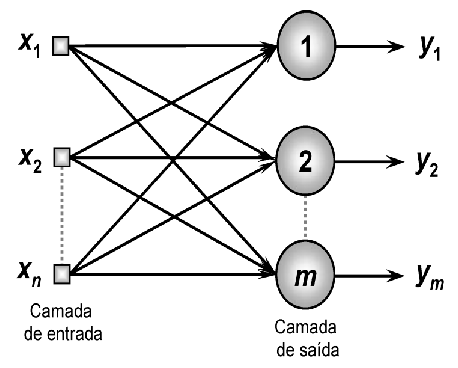
\includegraphics[width=85mm, height=50mm]{Figuras/Neural/pecepAdalin.png}\\
		\tiny Fonte: http://www.dkriesel.com. Acessado em: 10/10/2016
	      \end{figure}
	 %+++++++++++++++++++++++++++++++++++++++++++++++++++++++++++++++++++++++++++++++++++++++++++++++++++   
	      \item [(ii)] São exemplo dessas redes as de Perceptron multicamadas (PMC/MLP) e redes de base radial (RBF)
	      \begin{figure}[!ht]
		\centering
		\caption{Perceptron Multicamadas}
		\vspace{1mm}
		  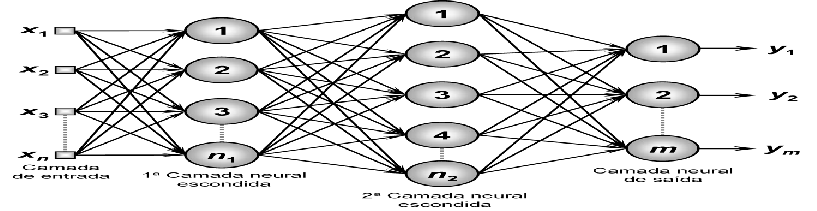
\includegraphics[width=110mm, height=70mm]{Figuras/Neural/MultiCamadas.png}\\
		\tiny Fonte: http://www.dkriesel.com. Acessado em: 10/10/2016
	      \end{figure}

	      Alguns autores ainda fazem referência às redes recorrentes ou realimentadas (iii), 
	      como a rede de Hopfield e a Perceptron multicamadas \cite{Kriesel2007NeuralNetworks}. 
	      Tais redes, segundo esses autores, são ideais para processamento dinâmico, como previsão de 
	      séries temporais, controle de processos, etc.
	      Referem também a existência das redes com estrutura reticulada (iv), como a rede de Kohone.
	%+++++++++++++++++++++++++++++++++++++++++++++++++++++++++++++++++++++++++++++++++++++++++++++++++++
	      \item [(iii)] Exemplo de rede recorrente ou realimentada: ``backpropagation''
	      \begin{figure}[!ht]
			\centering
			\caption{Perceptron com Realimentação}
			\vspace{1mm}
			  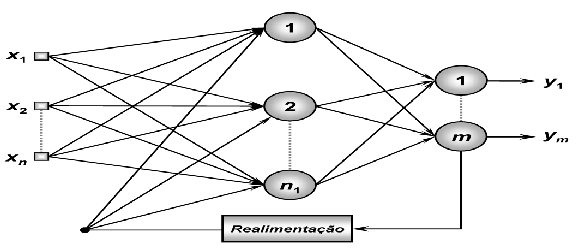
\includegraphics[width=100mm, height=65mm]{Figuras/Neural/Recorrentes.png}\\
			\tiny Fonte: http://www.dkriesel.com. Acessado em: 10/10/2016
	      \end{figure}  
	 
	 %+++++++++++++++++++++++++++++++++++++++++++++++++++++++++++++++++++++++++++++++++++++++++++++++++++   
	      \item [(iv)] Exemplo de redes de estrutura reticulada
	      \begin{figure}[!ht]
			\centering
			\caption{Rede Kohone}
			\vspace{1mm}
			  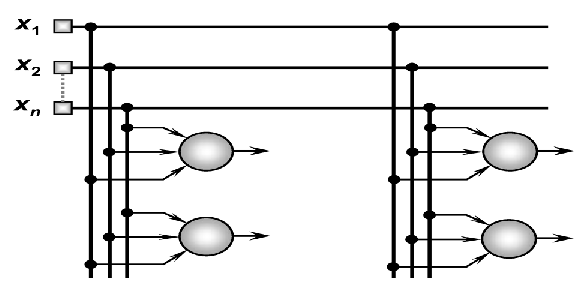
\includegraphics[width=100mm, height=65mm]{Figuras/Neural/Kohone.png}\\
			\tiny Fonte: http://www.dkriesel.com. Acessado em: 10/10/2016
	      \end{figure}
	
	\end{enumerate}

\pagebreak
	
  \item [(b)] Quanto às conexões, os tipos de RNA são: no sentido de ida; no sentido de ida e volta; 
	      lateralmente conectadas; topologicamente ordenadas; híbridas.
  
  \item [(c)] Quanto à aplicação: reconhecimento de padrões e classificação; processamento de imagem e visão; 
	      identificação de sistema e controle; processamento de sinais.
\end{itemize}


\subsubsection{Aprendizado em Redes Neurais}

O aprendizado caracteriza-se pela capacidade que a RNA tem de resolver uma determinada classe de problemas para os quais foi destinado 
seu desenvolvimento. 
Nesse processo, é proposto um algoritmo de aprendizado, que se caracteriza como um conjunto de regras bem delineadas que permitirão a 
resolução do problema. 

O aprendizado das RNA resulta da fase de treinamento, através de um processo iterativo de ajuste dos pesos. 
O conhecimento é armazenado nas sinapses, ou seja, nos pesos que são atribuídos às conexões que existem entre os neurônios da rede.

\begin{itemize}
 \item Por independência de quem aprende: o aprendizado pode ser por memorização, por contato, por exemplos, por analogias, por 
	exploração, por descoberta, sobretudo por uma mistura entre os últimos três \cite{Barreto2002}.
 \item Por retroação do mundo: quando há uma realimentação específica vinda do mundo exterior, podendo ser supervisionado ou 
	não-supervisionado. 
\end{itemize}

O treinamento supervisionado tem sido o mais comumente utilizado em redes neurais \cite{Barreto2002}. 
Em linhas gerais, como o nome indica, no treinamento supervisionado há um agente externo que indica explicitamente à rede um 
comportamento bom ou ruim, com base no padrão de entrada. Os valores iniciais dos pesos são aleatórios, e o ajuste se dá a partir do 
algoritmo de aprendizado, na próxima interação ou ciclo seguinte. São apresentados sinais de entrada e de saída à rede, e os ajustes 
vão sendo feitos paulatinamente. O treinamento pode levar um período considerável de tempo, em função dos ajustes que vão sendo 
realizados. O treinamento é concluído quando a rede neural atinge um determinado patamar de desempenho, tendo alcançado a precisão 
estatística esperada. 
Não havendo mais necessidade de treinamento, “congela-se” os pesos, para sua aplicação. 

O aprendizado não supervisionado, por sua vez, não depende de um agente externo, pois funciona de forma autorregulatória, apresentando 
mecanismos que analisam as regularidades ou tendências dos padrões de entrada, possuindo a capacidade de se adaptar automaticamente às 
necessidades da rede. 

O aprendizado de uma rede se dá em um determinado tempo e a partir de determinado padrão. 
A velocidade de aprendizado depende de variáveis que precisam ser consideradas como, por exemplo, a complexidade da rede proposta, 
a quantidade de camadas que ela possui, a arquitetura adotada, o algoritmo que foi utilizado, a precisão esperada. 
É preciso que se esteja atento a todos esses elementos, uma vez que dependendo de como essas variáveis forem consideradas, 
o treinamento pode se estender por um período bastante longo e, nem sempre apresentando um resultado satisfatório.

Quanto aos algoritmos de aprendizagem, são muitos os que podem ser utilizados, mas boa parte deles são variações do princípio de Hebb, 
que é a regra mais utilizada \cite{Barreto2002}. A descrição dessa regra foi apresentada pelo seu propositor, Donald Hebb, em 1949. 
A ideia básica dessa regra é a de que quando um neurônio recebe um entrada a partir de outro neurônio, isso significa que ambos 
estão ativos e que os pesos entre os neurônios precisam ser excitados.

Uma segunda lei utilizada é a de Hopfield. Ela se inspira no princípio de Hebb, mas acrescenta a ideia de definição da magnitude da 
excitação ou inibição. Uma terceira regra, que é a mais comumente utilizada hoje em dia, é a regra Delta de Widrow. 
Essa regra propõe a alteração dos pesos sinápticos, minimizando o erro quadrático da rede, reduzindo a diferença entre o valor de saída 
desejado e o atual valor de saída da unidade de processamento. 
Assim, o erro da saída é transformado pela derivação da função de transferência e utilizado pra regular os pesos de entrada da camada 
prévia da rede, realizando assim um processo de retropropagação dos erros. 
Para a utilização desse tipo de regra deve-se observar que o conjunto dos dados de entrada esteja organizado de forma aleatória. 

Há ainda a lei de aprendizado de Teuvo Kohonen, que foi inspirada em sistemas biológicos, em que há uma competição entre os elementos 
para aprender, ou atualizar e ajustar seus pesos. A unidade de processamento mais apta será aquela que possuir o melhor sinal de 
saída e terá a capacidade de inibir os ajustes sinápticos de seus concorrentes e excitar seus vizinhos, de maneira que apenas essa 
unidade e seus vizinhos poderão realizar o ajuste dos pesos.

%\subsection{Retropropagação e o Erro médio quadrático}


\section{Medida de desempenho e qualidade aplicadas à mineração}

Quando são desenvolvidos sistemas de predição e análise de diagnóstico, avalia-se o desempenho e a qualidade dos resultados encontrados.
Um método gráfico eficiente para detecção e avaliação da qualidade de sinais, conhecido como \textit{Receiver Operating Characteristic} -- ROC, ou curva ROC \cite{ROC},
foi criado e desenvolvido na década de 50 do século passado, para avaliar a qualidade da transmissão de sinais em um canal com ruído.
Recentemente a curva ROC tem sido adotada em Mineração de dados e Aprendizagem de Máquina \cite{MD_AM}, em sistemas de suporte à decisão na medicina, para analisar a qualidade da detecção 
de um determinado teste bioquímico, na psicologia para detecção de estímulos \cite{Discriminativo} em pacientes, e na radiologia para classificação de imagens.

Essas métricas são amplamente utilizadas na classificação binária de resultados contínuos. Para isso ser construído utiliza-se a Matriz de Contingência que classifica as probabilidades como:
verdadeiro positivo, falso positivo, falso negativo e verdadeiro negativo, respectivamente \textit{True Positive -- TP, False Positive -- FP, False Negative -- FN e True Negative -- TN },
também conhecida como matriz de confusão, descrita na tabela a seguir:

%tabela 5
\begin{table}[ht]
\centering
\caption{Matriz de Confusão}
\vspace{1mm}
\begin{tabular}{l|c|c}
\hline
\textbf{} & \textbf{Predito} & \textbf{}\\
\hline
\textbf{Real}  & TP   FN & Positive -- POS\\
\textbf{Real}  & FP   TN & Negative -- NEG\\
\hline
   ---         & PP   PN &    ---         \\
\end{tabular}
\\
\tiny Fonte: \cite{Bradley1997}
\end{table}

A matriz da Tabela 2.3 sintetiza a matriz da Tabela 2.4, portanto as duas tabelas são equivalentes.

%tabela 6
\begin{table}[ht]
\centering
\caption{Matriz modelo de Confusão}
\vspace{1mm}
\begin{tabular}{l|c|c}
\hline
\textbf{}           & \textbf{Y}     \textbf{$\bar{Y}$}   & \textbf{}\\
\hline
\textbf{X}          & P(X,Y)         P(X,$\bar{Y}$)       & Positive -- POS\\
\textbf{$\bar{X}$}  & P($\bar{X}$,Y) P($\bar{X},\bar{Y}$) & Negative -- NEG\\
\hline
   ---              & P(Y)           P($\bar{Y}$)         &     ---        \\
\end{tabular}
\\
\tiny Fonte: \cite{Bradley1997}
\end{table}


De acordo com as probabilidades condicionais temos:

\begin{equation}
 P(X,Y) = P(X|Y).P(Y) = P(Y|X).P(X)
\end{equation}

Então, a taxa de verdadeiros positivos será $P(Y|X)$ e a probabilidade de falsos alarmes ou taxa de falsos positivos será $P(Y,\bar{Y})$, a barra sobrescrita em $\bar{X}$
(ou $\bar{Y}$) representa negação. \\
A curva ROC será construída cruzando-se a taxa dos verdadeiros positivos (tpr = P(Y|X)) com a taxa dos falsos positivos (fpr = P(Y,$\bar{X}$)).

\pagebreak

\subsection{Classificação e Regressão para análise preditivas}

Classificação é um processo para encontrar um modelo que descreve e distingue classes de dados. 
Esse modelo tem como base de análise um conjunto de treinamento (i.e. objetos de dados para os quais 
serão encontrados rótulos que os classifiquem). 

Esse modelo é usado para predizer quais rótulos de classes terão os objetos desconhecidos.
O modelo pode ser representado por regras de classificação do tipo ``IF - THEN'', por árvores de decisão, redes neurais e outros. 
Regras de classificação se distinguem de regras de indução da seguinte forma:
\begin{itemize}
	\item Uma regra de classificação poderia ser: $if$ L $them$ class = $C_{1}$ ou $if$ L $them$  $C_{1}$
	\item Uma regra de indução seria: $ if$ L $them$ R que por sua vez produz novas regras 
\end{itemize}

%\singlespace
\vspace{2cm}

\begin{figure}[ht] \unitlength= 1mm \thicklines
	\centering{
		\begin{picture}(100,6)
		\put(0,0){\framebox(115,6)} \put(3,2){$age(X,``youth")$ AND $income(X,``high")  \to classe (X,``A")$}
		\put(0,-7){\framebox(113,6)} \put(3,-5){$age(X,``youth")$ AND $income(X,``low") \to classe (X,``B")$}
		\put(0,-14){\framebox(85,6)} \put(3,-12){$age(X,``middle-aged")$  $\to classe (X,``B")$}
		\put(0,-21){\framebox(70,6)} \put(3,-19){$age(X,``senior")$  $ \to classe (X,``B")$}
		\end{picture}
	}
\end{figure}

\vspace{3cm} 

A figura a seguir representa uma rede neural com as mesmas características da árvore de decisão anterior:
\begin{figure}[!ht]
	\centering
	\caption{Rede Neural}
	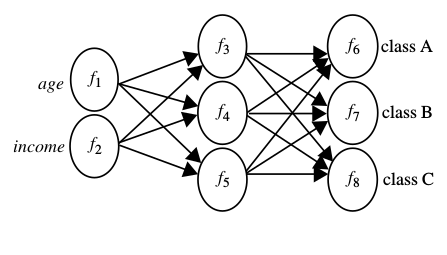
\includegraphics[width=85mm, height=38mm]{Figuras/BigData/redeneural.png}\\
	\tiny Fonte: Han, J. and Kamber, M. 
\end{figure}  

As árvores de decisão produzem regras de indução, são algoritmos rápidos, contudo dados impuros podem comprometer o desempenho desse algoritmo. 
A fase de extração dos dados do é fortemente influenciáveis pelas variáveis escolhidas, \cite{DecisionTree} 
isso pode representar o desafio maior para implementar esta técnica. 

Outro problema que pode ser encontrado em algoritmos de aprendizagem é o ``overfitting'' ou superadaptação aos modelos.
Segundo RUSSEL E NORVIG (2004)  \footnote{Foi observado que redes neurais muito grandes \textit{generalizam} bem, 
\textit{desde que os pesos sejam mantidos pequenos}. Essa restrição mantém os valores de ativação na região 
\textit{linear} da função sigmóide g(x) onde x é próximo de zero. Por sua vez isso faz com que a rede se comporte 
como uma função linear, com um número muito menor de parâmetros.} o ``overfitting'' ocorre quando o número atributos é grande.


  \chapter{Metodologia}\label{meto}

O processo para construir o modelo preditivo foi o CRISP -- DM. forneça informação suficiente a um gestor para decidir quando e por onde 
enviar uma frota de caminhões por determinada rodovia que apresente retenções crescentes de logística de cargas. As soluções disponíveis que 
existem tais como; Google Maps, Waze e outros dessa natureza somente exibem informações momentâneas, produzidas e compartilhadas pelos utilizadores 
dos aplicativos ou por informações provindas de GPS, contudo não analisam dados históricos dessas rodovias nem fazem predições futuras sobre o 
comportamento delas. \\

\section{Plano geral da metodologia}

A metodologia da pesquisa contempla um plano em três etapas, cada uma dividida em fases atinentes.
As duas primeiras etapas da nossa metodologia completam o ciclo do processo CRISP-DM.
A terceira etapa é o ``front-end'', onde são plotados no mapa os pontos críticos da rotas.

\pagebreak

A figura a seguir ilustra essa metodologia descrita graficamente, onde as três etapas são representadas por retângulos.
 
\begin{figure}[ht]
\centering
\caption{Etapas da gerais da metodologia}
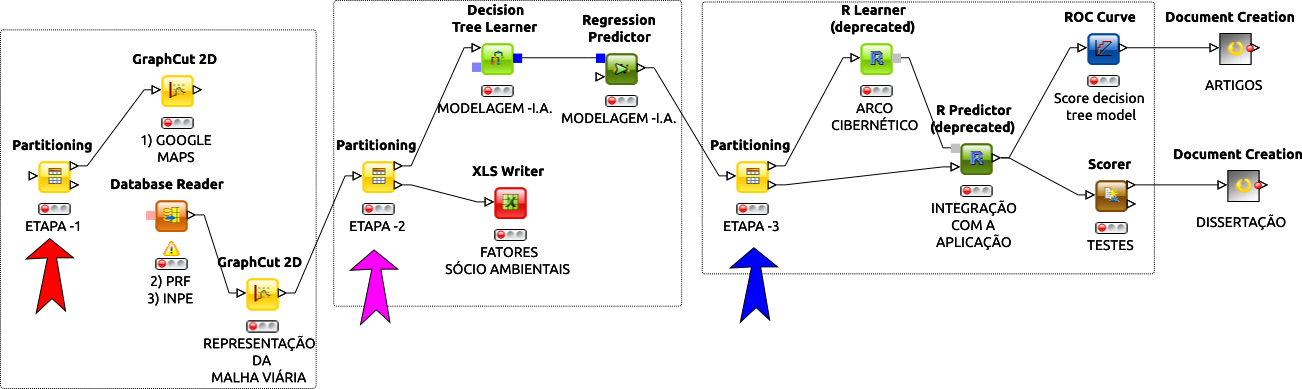
\includegraphics[width=160mm, height=70mm]{Figuras/BigData/Etapas.png}
\end{figure}

A \textbf{etapa 1} contempla a fases da coleta das bases de dados históricas, preparação dos dados e construção das variáveis do modelo preditivo.
\begin{enumerate}
 \item O modelo preditivo integra várias bases de dados, tais como: Polícia Rodoviária Federal -- PRF, Batalhão de Polícia de Transito -- BPRv e dados históricos 
       do Instituto de Pesquisas Espaciais -- INPE ou dos dados de precipitações pluviométricas do ``European Centre for Medium-Range Weather -- ECMWF.
 
 \item Algumas dessas informações também estão disponíveis em base de dados abertas, como sugere o Portal da Transparência, nos servidores da PRF além de outras informações para complementar o sistema estão 
       disponíveis na Internet sendo atualizadas pela PRF através de uma API aberta, esta pode ser configurável para se ligar ao nosso sistema.
\end{enumerate}

 
O segunda \textbf{etapa 2} consiste na Mineração dos dados, tendo como ''inputs`` a etapa anterior; aplicar as técnicas de IA nas variáveis do sistema preditivo.
%Propomos inicialmente a Regressão Logística e Árvores de decisão, testes iniciais e depuração do modelo. transformar os dados provenientes do modelo preditivo em coordenadas geográficas, isto é:
Os ''outputs`` dessa etapa consiste em transformar os dados provenientes mineração em coordenadas geográficas, isto é: em latitude e longitude.  
 
A \textbf{terceira} e última etapa da metodologia contempla:
 \begin{enumerate}
  \item A malha viária representada em mapas de bases vetoriais;
  \item Um ambiente de simulação interativa que utiliza uma plataforma baseada na API do Google Maps.
  \item Um módulo dinâmico onde são capturados ``feeds'' de redes sociais, por exemplo pelo Twitter. 
	Essa técnica faz um arco cibernético mantendo o sistema atualizado.
\end{enumerate}

As coordenadas geográficas, ``outputs'' da etapa 2, são agrupadas a priori formando ''cluster`` de dados 
a serem exibidos nos mapas vetoriais das APIs correspondentes.

A representação da malha viária, que acopla a estrutura dinâmica com a estrutura estática, é o ``front-end'' da metodologia. 
Esta etapa permite uma contraposição ao modelo preditivo na perspectiva do usuário gestor. 
Isso pois, modelos preditivos com o passar do tempo tendem a desfasar-se, contudo este módulo permite visualização
instantânea do ambiente das rodovias. 
 


\section{Modelo preditivo}

O modelo preditivo foi construído utilizando bases de dados históricas da PRF (de acidentes e de paralisações ex: protestos) entre Janeiro de 2007 a 
Dezembro 2015. As bases de dados do Batalhão de Polícia de Rodoviária estadual -- BPRv vieram entre Janeiro/2010 a Julho/2016, cortes em ambas as bases foram 
feitos para adequar as datas. Essas bases de dados são integradas gerando um único e complexo modelo preditivo que será acoplado a estrutura dinâmica.


%\pagebreak

\section{Reflexão sobre as tecnologias utilizadas no modelo preditivo}\label{result}

Não existe uma técnica de mineração que generalize os mais diversos ambientes preditivos, mas sim um ``pool'' dessas técnicas onde uma complementa outra.

As técnicas preditivas tradicionais que contemplam análise de grandes massas de dados como base homogêneas.

são possíveis quando adaptadas para uma forma comparável à que
foram inicialmente concebidas, por que as variáveis em uma base de dados a priori guardam pouca relação as variáveis de outra base de dados.
neste caso essas variáveis ou são excluídas ou são transformadas a fim de ``guardarem'' um correlação com a outra base de dados. 

Na fase de transformação de dados, onde são criadas novas variáveis, a proximidade entre as
bases heterogêneas deverão se estreitam. 
Nesta pesquisa, bases heterogêneas foram integralizadas num única grande base, onde as variáveis independentes foram
em sua maioria preservadas e/ou construídas novas, nas bases onde não haviam correspondência, respeitando a lógica do negócio.\\
A tabela a seguir descreve as variáveis originais na base de dados de acidentes da PRF 


\section{Extração do conhecimento}

As técnicas como Redes Neurais Artificias (MLP) [\large{CITAR}], Árvores de decisão (CART) [\large{CITAR}], Regressão logística (MLR) 
[\large{CITAR}] fornecem visão generalizada dos fatores preponderantes, levantando padrões ocultos nos dados. Esta fase é conhecida como 
Aprendizagem de Máquina (acrônimo de Machine Learning)

\begin{itemize}
 \item[a] Redes Neurais Artificias do tipo \textit{ Multi Layer Perceptron}  -- (MLP) têm capacidade de receber várias entradas ao mesmo tempo e distribuí-las de maneira organizada, além 
	  são simples de implementar e trazem resultados satisfatórios em grandes bases de dados.
 
 \item[b] Árvores de decisão para classificar acidentes do tipo \textit{ Classification and Regression Tree}  -- (CART) foi empregue por Pakgohar et al no artigo 
	  \textit{The role of human factor in incident and severity of road crashes based on the CART and LR regression a data mining approach}  com nível de acurácia próximo aos 80\%

 \item[c] Regressão logística tipo \textit{Multinomial Logistic Regression} -- (MLR) fornece a possibilidade de aprofundamento em vários níveis de busca sendo a mais apropriada, já que Regressão logística 
	  tradicional não permite aprofundamento desse tipo no espaço de busca.
\end{itemize}


\pagebreak

\section{Acoplamento com a estrutura dinâmica}

A estrutura dinâmica é composta por duas API's, uma disponibilizada pela Google, através do Google Maps que está atualmente na versão V3 e 
outra uma API do Twitter. A API do Google Maps proporciona uma ``leitura'' atualizada em forma de mapa no momento em que a estrutura dinâmica ``roda''. 

A API do Twitter também tem a possibilidade de atualizar o modelo preditivo, contudo o objetivo desta é faz um Arco cibernético, 
retroalimentando todo o sistema com novas informações, pensamos que isso permite um visualização instantânea do ambiente como um todo.

Os ``feeds'' das redes sociais como o Twitter permitem analisar o contexto das rodovias com defasagem temporal 
pequena, os utilizadores dessas redes sociais inclusive a PRF atualizam as redes sociais com dados sempre que há uma ocorrência por essas 
A monitoração dessas redes sociais se faz por Mineração em textos, são verificas palavras chaves como: protestos, acidentes e outras.



\begin{figure}[ht]
\centering
\caption{Etapas da metodologia}
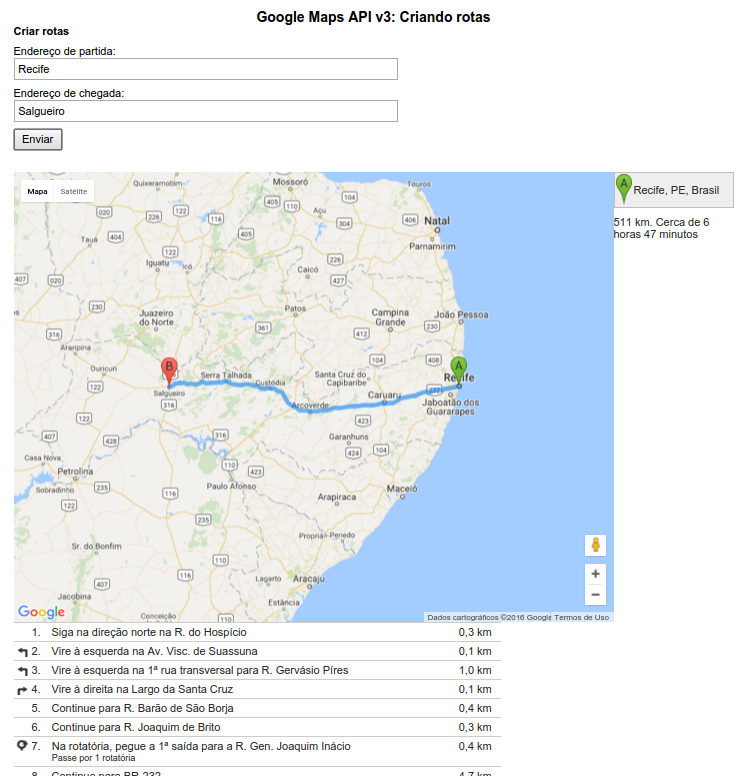
\includegraphics[width=150mm, height=130mm]{Figuras/Cronograma/GoogleMaps.png}
\end{figure}
  \chapter{Simulação}\label{simula}

\section{Execução do modelo}

Esse capítulo apresenta os resultados encontrados em cada etapa, no processo de desenvolvimento do modelo de predição de ocorrências nas principais BRs do estado de Pernambuco, para definição de melhores rotas e horários para os usuários dessas vias.

\vspace{5mm}

A figura a seguir resume as três etapas contempladas na proposição do modelo.

\begin{figure}[ht]
\centering
\caption{Etapas da modelo proposto}
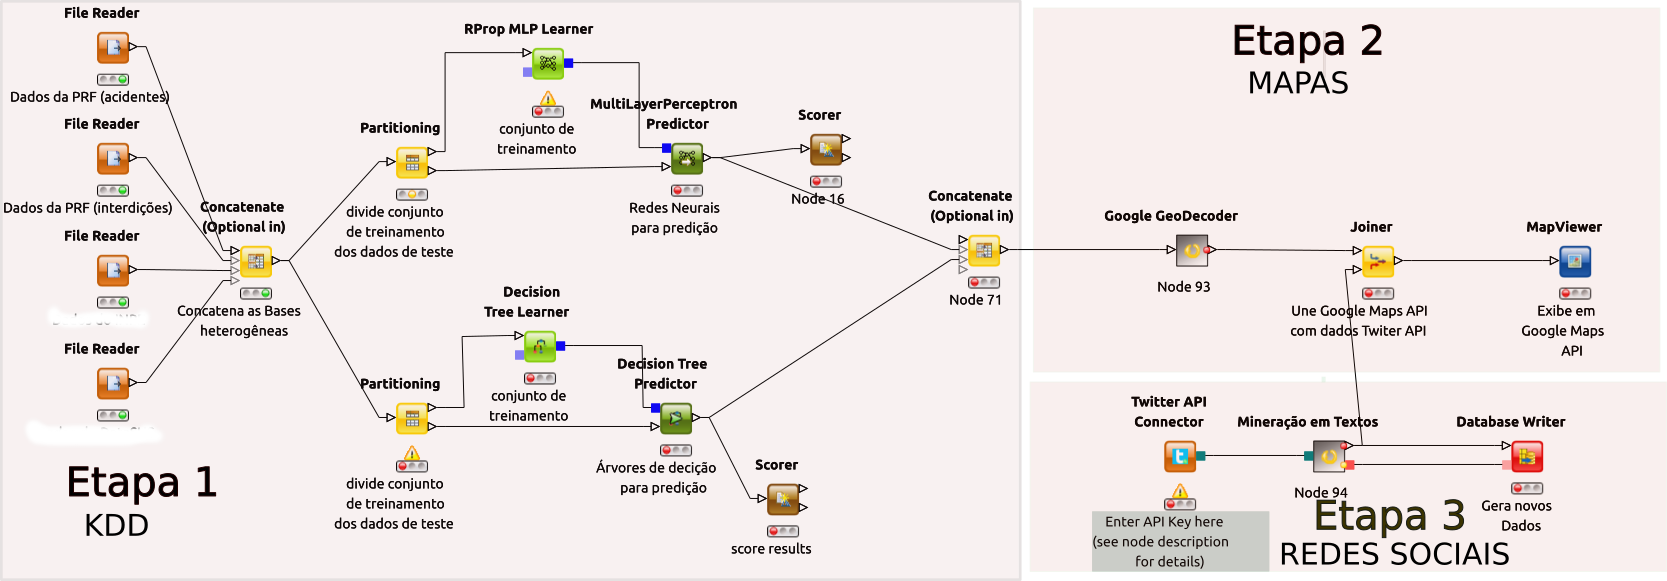
\includegraphics[width=175mm, height=75mm]{Figuras/Cronograma/metodologia.png}\\
\tiny Fonte: autor
\end{figure}

A \textbf{etapa 1} contempla a fase da coleta das bases de dados históricos, preparação dos dados, construção das variáveis do modelo preditivo, descoberta dos pontos críticos das rodovias (que serão utilizados na etapa de georreferencaimento).
  \begin{enumerate}
    \item O modelo preditivo integra as bases de dados da Polícia Rodoviária Federal -- PRF.
 
    \item Algumas dessas informações também estão disponíveis em base de dados abertas, como sugere o Portal da Transparência, nos servidores da PRF, além de outras informações complementares.
    \item A conclusão dessa etapa ocorre com a Mineração dos dados e a extração de conhecimento.
	  Os ''outputs`` dessa etapa consistem nos pontos críticos localizados nas rodovias, que permitem traçar uma rota. 
	  As localizações geográficas, indicadas pelo Km, são agrupadas formando ''clusters`` de dados exibidos em mapas vetoriais. 
	  A partir da definição dos pontos críticos foram geradas matrizes -- de mortos e de gravidade -- que serviram para localizar tais pontos no mapa e traçar rotas.
	  As principais ferramentas de I.A. utilizadas nessa etapa foram Árvores de Decisão e Redes Neurais, com a finalidade classificar e predizer os pontos críticos em cada quilômetro das rodovias.\\
\end{enumerate}
  
A \textbf{segunda} etapa contempla:
 \begin{enumerate}
 	\item Um módulo dinâmico onde são capturados ``feeds'' da rede social Twitter. 
 	     Essa técnica faz um arco cibernético mantendo o utilizador atualizado com as informações recentes. 
  \end{enumerate}

A \textbf{terceira} e última etapa consiste em um módulo com as seguintes características:
  \begin{enumerate}
    \item Representação da malha viária em mapas de bases vetoriais;
    \item Um ambiente de simulação interativa que utiliza uma plataforma baseada na API do Google Maps.
    \item Quando houver informações vindas do twitter sobre ocorrências na rodovia, deverá ser feita a geolocalização
  \end{enumerate}


\section{A construção do Modelo preditivo}

O modelo preditivo foi construído utilizando bases de dados históricos da PRF (de acidentes e de paralisações, por exemplo,  protestos) entre Janeiro de 2007 a Dezembro 2015. Cada ano correspondia a uma base de dados independentes, tendo sido integradas, formando uma base única com aproximadamente 85 mil registros. 


\subsection{Aplicação do CRISP-DM}
O CRISP-DM nesta pesquisa ajudou a guiar as escolhas nos momentos em que os resultados pareciam não fazer sentido. Todavia, por ser um processo recursivo, o retorno aos fundamentos dessa metodologia prevê que haja ajustes necessários, a fim de se atingir os objetivos da proposta.

A proposta metodológica delineada para esta pesquisa contemplou todas as fases do KDD, conforme descrito a seguir.

\subsubsection{Fases da Mineração ao KDD}

Seleção: Nesta etapa foram coletadas as informações provenientes das bases de dados da Policia Rodoviária Federal de Pernambuco entre 2007 e 2015. Segundo informações da própria PRF/PE, apenas a partir de 2007 esses dados passaram a ser armazenados eletronicamente. A PRF/PE dispõe em banco de dados relacionais alguns desses dados na Internet,
contudo no artigo “Uma análise da qualidade dos dados relativos aos boletins de ocorrências das rodovias federais para
o processo de Mineração de Dados”, COSTA, BERNARDINI, LIMA \cite{Costa2015} destacam a não padronização e não aceitação dos
dados pela comunidade internacional. EAVES, D. \cite{Eaves} sugere que os dados sejam disponibilizados na maneira como foram
coletados. 

A primeira base de dados coletada diretamente dos servidores da PRF continha relatório de acidentes e a segunda a de interdições. A partir dos dados capturados na base da PRF utilizamos como variáveis de entrada:

\begin{itemize}
 \item Condição da Pista: {Seca, Com buracos, Molhada, Em obras, Com material granulado, Oleosa, Enlameada, Com gelo, Outras}
 \item Restrição de visibilidade: {Inexistente, Veículo Estacionado, Poeira/Fumaça/neblina, Vegetação, Ofuscamento, Cartazes/faixas, Placas}
 \item Traçado da via: {Reta, Curva, Cruzamento, Defeito}
 \item Tipo de veículo: {Automóvel, Caminhonete, Motocicletas, Caminhão, Caminhão-trator, Bicicleta, Ônibus, Motoneta, Micro-ônibus, Trator de rodas, Carroça, Caminhão-Tanque, Semi-Reboque, Utilitário, Ciclomotor, Charrete, Carro-de-mão, Quadriciclo, Trator misto, Reboque, Trator de esteiras, Não informado, Não se aplica, Não identificado}
\end{itemize}

Preprocessamento: Nesta fase foram retiradas as variáveis que continham inconsistência e “missing data”, como, por exemplo, informações acerca de latitude e longitude. Cabe destacar que a base de dados, como um todo, apresentava sérias inconsistências, uma vez que, por exemplo,
um mesmo acidente, quando envolvia dois ou mais veículos,
era lançado na base duas ou mais vezes, em função da
quantidade de veículos envolvidos. Foram eliminadas variáveis
em duplicidade (i.e. as variáveis Mês, Ano que apareciam
separadamente, já haviam sido contempladas na variável Data.).

Transformação: Foram criadas as variáveis “Tipo de
paralisação”, contemplando acidentes sem mortos e com, no
máximo, dois veículos envolvidos; “Dias da semana”
(domingo, segunda-feira,....sábado); “Ajuste de horas” (i.e. 17h58, 17h59, 18h, 18h01, 18h02, arredondadas para 18h);
“Ajuste de Km” (seguiu a mesma lógica do ajuste de horas).

Mineração de dados: O algoritmo escolhido para essa fase da pesquisa
foi Árvore de Decisão, que possibilita uma interpretação
imediata e de fácil compreensão. Como ferramentas, foram
escolhidas o Knime \cite{Knime}, R \cite{R-cran} e Weka \cite{Weka}, com objetivo
de estabelecer uma comparação entre eles, cuja intenção era
produzir um classificador mais robusto. Nessa direção, a
técnica Ensamble de classificadores \cite{Bernardini} estabelece que a
combinação de um ou mais classificadores iguais, ou mais de
um classificador diferente, aumenta a precisão. 

Tanto na ferramenta Knime como Weka o algoritmo de árvore de decisão é chamado de J48,
uma vez que se trata da implementação Java do algoritmo
C4.5 no R. A biblioteca “rparty” implementa esse algoritmo.

Para escolha das variáveis de entrada foi calculada a correlação linear entre todas as variáveis. Entre as variáveis BR e
Delegacia (variável que agrega municípios) obteve-se correlação linear de 0,653. Entre Tipo de Acidente e Traçado via a
correlação foi baixa, apenas 0,14. Variáveis com correlação linear abaixo disso foram descartadas. 

Outra métrica para a escolha de variáveis de entrada foi a entropia, que é um elemento considerado importante pela literatura \cite{NorvigRussel2004}. Nesse caso, variáveis que seriam desconsideradas em virtude da baixa correlação linear, foram reconsideradas por conta da entropia.

Interpretação/Avaliação: Produção de árvores de decisão a
partir do estabelecimento de diferentes nós-raízes, definidos em
virtude da correlação linear e/ou da entropia.

\pagebreak

%++++++++++++++++++++++++++++++++++++++++++++++++++++++++++++++++++++++++++++++++++++++++++++++
\subsection{Dados encontrados antes da Mineração}

Os dados revelaram que a grande maioria dos acidentes ocorre com pista seca, sem restrição de visibilidade. 
A cor vermelha remete aos trechos BR 101 em que ocorrem mais acidentes. A cor azul diz respeito à menor frequência de acidentes.

\begin{figure}[h]
	\caption{BR 101: Hora do acidente (1) Concentração em torno da hora (2)}
	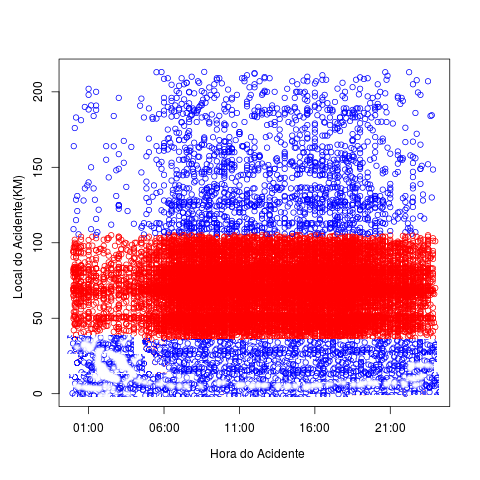
\includegraphics[width=7cm,height=7cm]{Figuras/Preprocess/br101.png}
	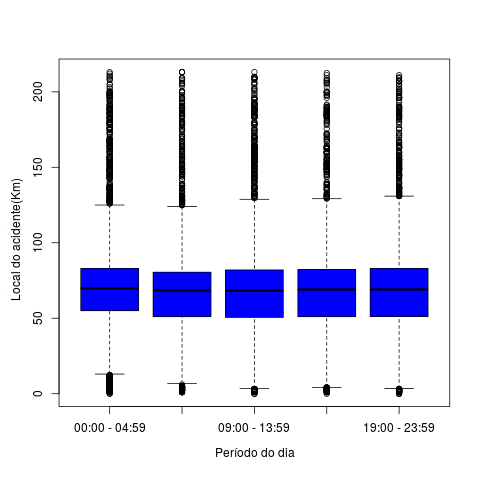
\includegraphics[width=7cm,height=7cm]{Figuras/Preprocess/br101_2.png}
	
\end{figure}

\quad \quad
\begin{figure}[h]
	\centering
	\caption{ Frequência}
	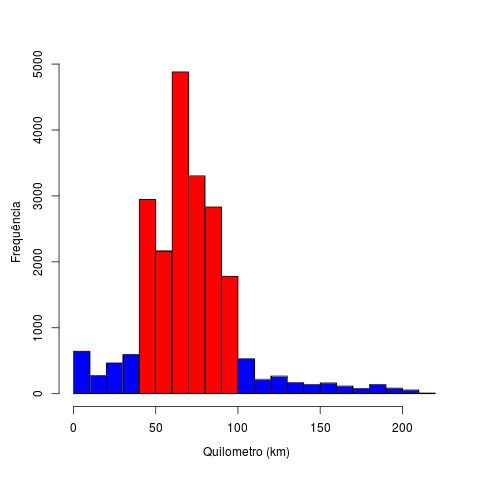
\includegraphics[width=7cm,height=7cm]{Figuras/Preprocess/br101_4.png}
\end{figure}

O gráfico 4.2(1), 4.2(2)  e 4.3 contêm dados da BR 101, uma das mais importantes para o nordeste brasileiro, uma vez que atravessa a maioria dos estados dessa região, nas localidades mais densamente povoadas. Em virtude disso, seu tráfego intenso. 
A gráfico 4.2(1) representa os acidentes que ocorreram a cada hora (abcissa) em cada Km (ordenada) nos últimos nove anos. 
O  gráfico 4.2(2) corresponde à frequência do local onde ocorreram esses acidentes. 
É possível perceber que há determinados locais na rodovia onde se concentram os acidentes. 
O terceiro gráfico, tipo ‘boxplot’, exibe a concentração das ocorrências em torno da mediana dessa localidade (Km). 
Especulou-se, a priori, que a variável “traçado da rodovia” ou que as condições climáticas poderiam ser de grande influência na ocorrência de acidentes, contudo mais adiante descobrimos outros condicionantes que influenciam mais fortemente esses acontecimentos. 
É possível perceber no gráfico 4.2(1) e no 4.3 que especialmente em determinados locais (Km) -- por exemplo na BR 101, entre os Km 40 e 100 -- os acidentes ocorrem desde as 05h da manhã até as 23h. 



\begin{figure}[h]
	\caption{BR 104: Hora do acidente (1) Concentração em torno da hora (2)}
	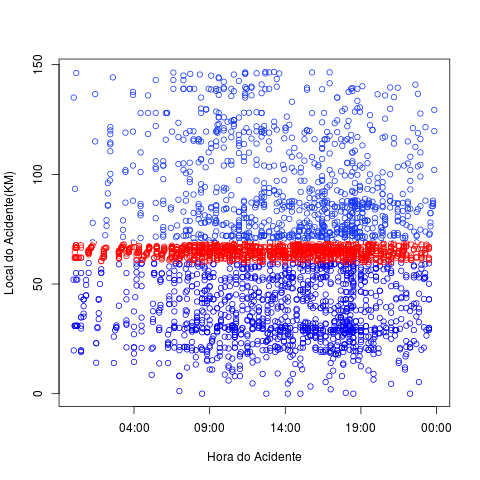
\includegraphics[width=7cm,height=7cm]{Figuras/Preprocess/br104_12.png}
	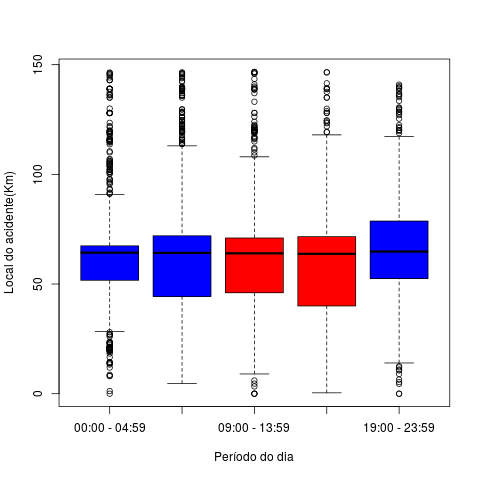
\includegraphics[width=7cm,height=7cm]{Figuras/Preprocess/br104_2.png}

\end{figure}

\quad \quad
\begin{figure}[h]
	\centering
	\caption{ Frequência}
	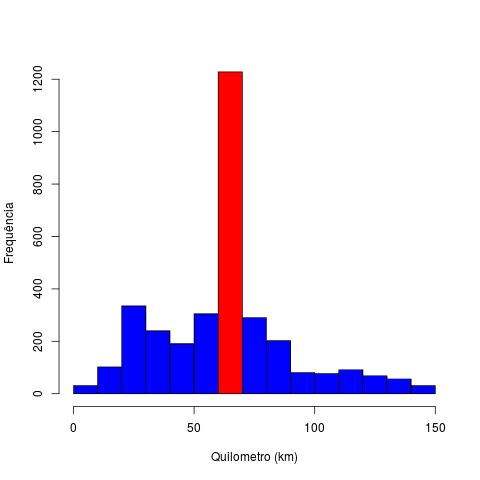
\includegraphics[width=7cm,height=7cm]{Figuras/Preprocess/br104_3.png}
\end{figure}

O gráfico 4.4(1), 4.4(2) e 4.5 apresentam dados da BR 104, que atravessa seis municípios de Pernambuco, dentre eles Caruaru, que é responsável por uma das maiores frotas de veículos do interior e por onde passam cerca de 50 mil veículos por dia. 
A gráfico 4.4(1) representa, nos últimos nove anos, os acidentes que ocorreram a cada hora (abcissa) em cada Km (ordenada).
O  gráfico 4.4(2) corresponde à frequência do local onde ocorreram esses acidentes. 
Percebe-se que em torno do Km 60 concentra-se o maior número de ocorrências. 
O terceiro gráfico (boxplot) apresenta as ocorrências em torno da mediana dessa localidade (Km). 
No gráfico 1 são identificados padrões, por exemplo no Km 60 ocorrem acidentes que se estendem das 04h às 23h. 


\pagebreak
%++++++++++++++++++++++++++++++++++++++++++++++++++++++++++++++++++++++++++++++++++++++++++++++

\begin{figure}[h]
	\caption{BR 110: Hora do acidente (1)  Concentração em torno da hora (2)}
	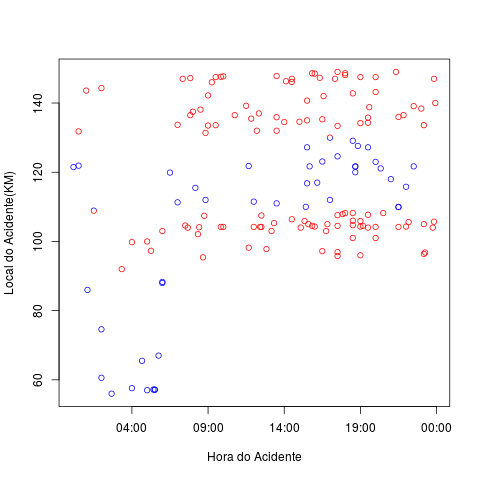
\includegraphics[width=7cm,height=7cm]{Figuras/Preprocess/br110_1.png}
	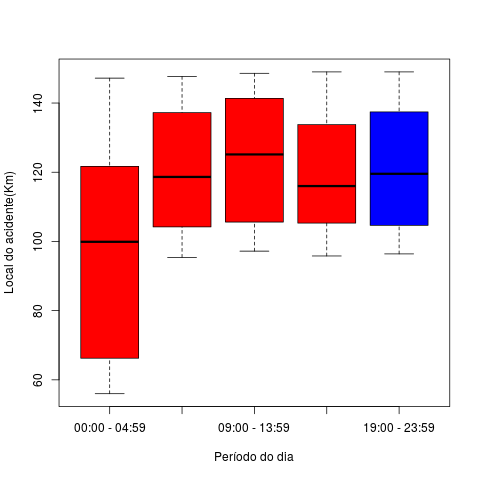
\includegraphics[width=7cm,height=7cm]{Figuras/Preprocess/br110_2.png}

\end{figure}


\quad \quad
\begin{figure}[h]
	\centering
	\caption{ Frequência}
	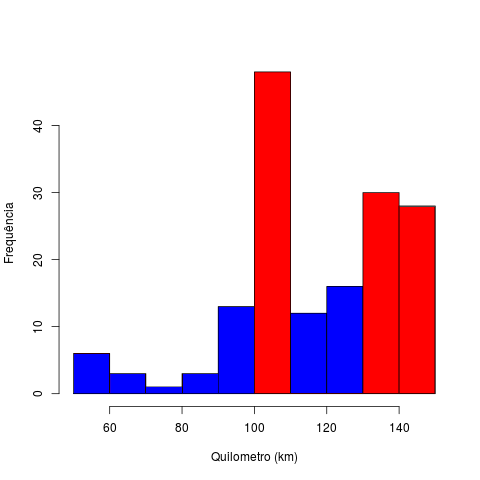
\includegraphics[width=7cm,height=7cm]{Figuras/Preprocess/br110_3.png}
\end{figure}

\pagebreak
%++++++++++++++++++++++++++++++++++++++++++++++++++++++++++++++++++++++++++++++++++++++++++++++

\begin{figure}[h]
	\caption{BR: 116 Hora do acidente (1) Concentração em torno da hora (2)}
	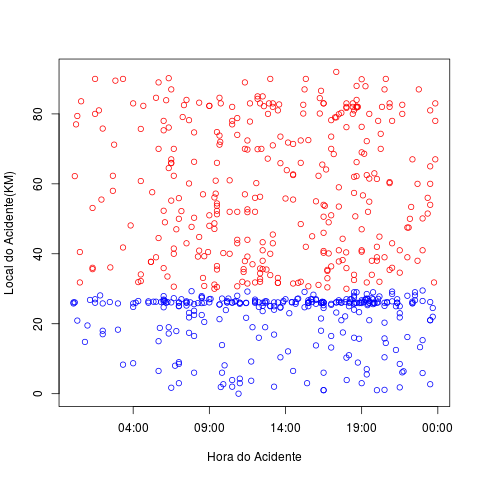
\includegraphics[width=7cm,height=7cm]{Figuras/Preprocess/br116_1.png}
	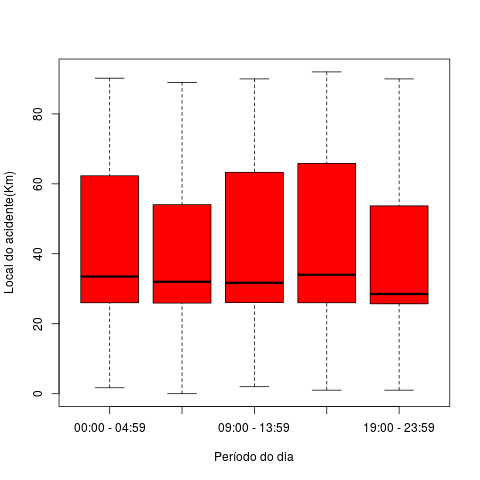
\includegraphics[width=7cm,height=7cm]{Figuras/Preprocess/br116_2.png}

\end{figure}

\quad \quad
\begin{figure}[h]
	\centering
	\caption{ Frequência}
	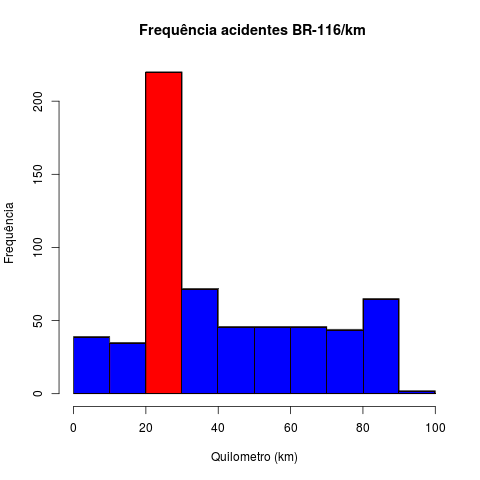
\includegraphics[width=7cm,height=7cm]{Figuras/Preprocess/br116_3.png}
\end{figure}

O gráfico 4.8(1), 4.8(2)  e 4.9 apresentam dados da BR 116, que percorre os estados do Brasil que vão desde o Rio Grande do Sul até o Ceará. O gráfico 4.8(1) mostra os acidentes que ocorreram a cada hora (abcissa) em cada Km (ordenada), também nos últimos nove anos. 
O  gráfico 4.8(2) corresponde à frequência do local onde esses acidentes aconteceram. Há determinados locais na rodovia em que a maioria dos acidentes se concentram. 
O gráfico tipo ‘boxplot’ exibe a concentração das ocorrências em torno da mediana dessa localidade (Km). 
Inicialmente acreditou-se que a variável “traçado da rodovia” ou que as condições climáticas poderiam ter grande influência na causa dos acidentes. Entretanto, mais adiante foram descobertos outros condicionantes dessas ocorrências. 
É possível perceber no gráfico 4.9, que os acidentes em torno do Km 30 ocorrem com mais frequência a partir da 04h da manhã, estendendo-se até próximo às 22h. 

\pagebreak
%++++++++++++++++++++++++++++++++++++++++++++++++++++++++++++++++++++++++++++++++++++++++++++++

\begin{figure}[h]
	\caption{BR 232: Hora do acidente (1)  Concentração em torno da hora (2)}
	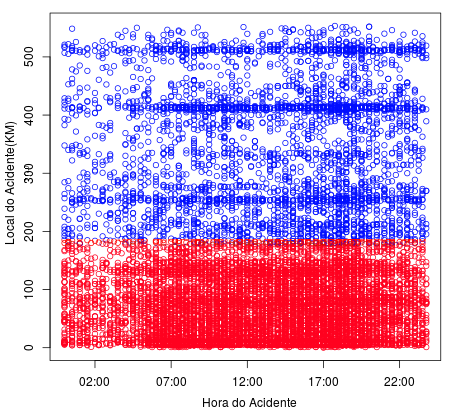
\includegraphics[width=7cm,height=7cm]{Figuras/Preprocess/br232_1.png}
	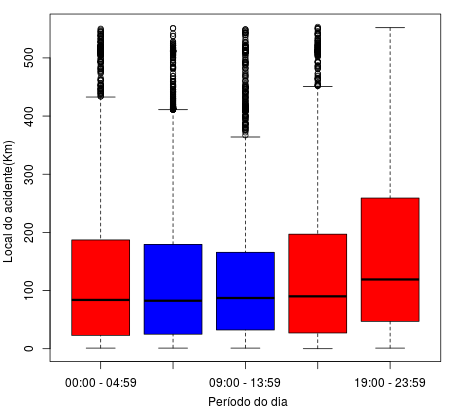
\includegraphics[width=7cm,height=7cm]{Figuras/Preprocess/br232_32.png}

\end{figure}

\quad \quad
\begin{figure}[h]
	\centering
	\caption{ Frequência}
	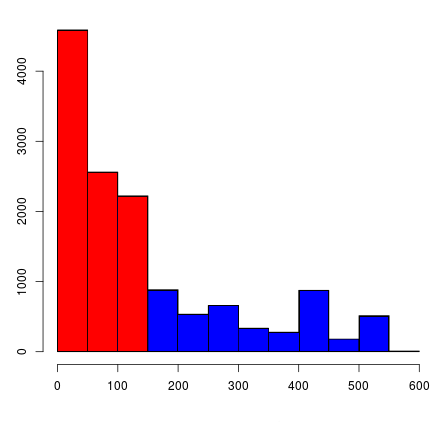
\includegraphics[width=7cm,height=7cm]{Figuras/Preprocess/br232_3.png}
\end{figure}

O gráfico 4.10(1), 4.10(2)  e 4.11 trazem dados da BR 232, cuja importância se destaca pelo fato de atravessar todo o estado de Pernambuco, de leste a oeste. O primeiro gráfico apresenta os acidentes dos últimos nove anos, em cada hora (abcissa) e Km (ordenada). O  gráfico 4.10(2) corresponde ao local onde aconteceram esses acidentes. É possível perceber no gráfico 4.11, que nessa BR há um número maior de acidentes nos Km 0, 90, 110, 260, 410 e 500, desde a 00h até as 23h. O terceiro gráfico (‘boxplot’) exibe a concentração das ocorrências em torno da mediana dessa localidade (Km). 
Especulou-se a priori que a variável “traçado da rodovia” ou que as condições climáticas eram as principais responsáveis pelo grande número de acidentes.



\pagebreak
%++++++++++++++++++++++++++++++++++++++++++++++++++++++++++++++++++++++++++++++++++++++++++++++

\begin{figure}[h]
	\caption{BR 316: Hora do acidente (1) Concentração em torno da hora (2)}
	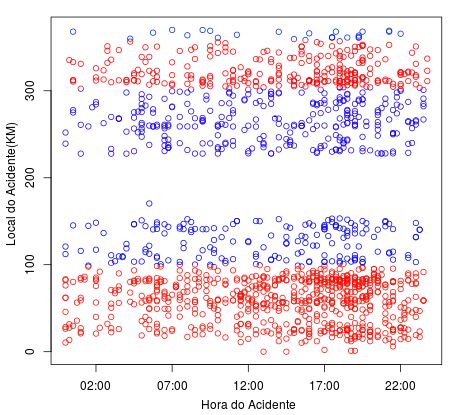
\includegraphics[width=7cm,height=7cm]{Figuras/Preprocess/br316_1.png}
	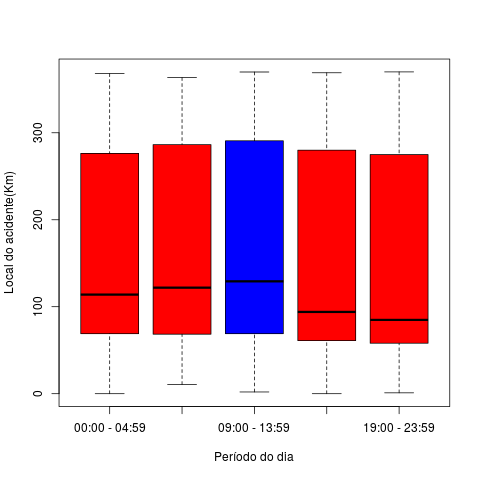
\includegraphics[width=7cm,height=7cm]{Figuras/Preprocess/br316_2.png}

\end{figure}

\quad \quad
\begin{figure}[h]
	\centering
	\caption{ Frequência}
	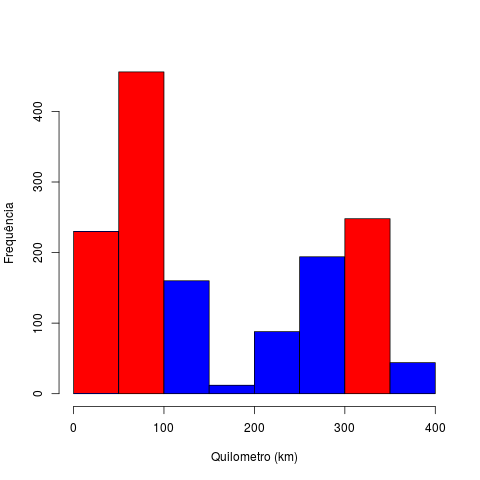
\includegraphics[width=7cm,height=7cm]{Figuras/Preprocess/br316_3.png}
\end{figure}

O gráfico 4.12(1), 4.12(2)  e 4.13 trazem dados da BR 316. Esta BR é uma das menores do Estado de Pernambuco, de oeste a leste. O primeiro gráfico apresenta uma área em branco no centro, os acidentes se concentram nas extremidades, no entorno do km 90 e 300 (da abcissa) e acontecem com maior frequência em torno das 17h00 (ordenada).

\pagebreak
%++++++++++++++++++++++++++++++++++++++++++++++++++++++++++++++++++++++++++++++++++++++++++++++

\begin{figure}[h]
	\caption{BR 407: Hora do acidente (1) Concentração em torno da hora (2)}
	\includegraphics[width=7cm,height=7cm]{Figuras/Preprocess/br407_1.png}
	\includegraphics[width=7cm,height=7cm]{Figuras/Preprocess/br407_3.png}

\end{figure}

\quad
\begin{figure}[h]
	\centering
	\caption{ Frequência}
	\includegraphics[width=7cm,height=7cm]{Figuras/Preprocess/br407_2.png}
\end{figure}

Na BR 407 os acidentes se concentram na altura do Km 130, representados nos gráficos 4.14 (1) e 4.14 (2).
Esta BR situa-se no extremo oeste do Estado, ligando a cidade de Afrânio a Petrolina. A peculiaridade desse trecho (km 130) é verificada na descida da ponte que atravessa o rio São Francisco.

\pagebreak
%++++++++++++++++++++++++++++++++++++++++++++++++++++++++++++++++++++++++++++++++++++++++++++++

\begin{figure}[h]
	\caption{BR 408: Hora do acidente (1) Concentração em torno da hora (2)}
	\includegraphics[width=7cm,height=7cm]{Figuras/Preprocess/br408_1.png}
	\includegraphics[width=7cm,height=7cm]{Figuras/Preprocess/br408_2.png}

\end{figure}

\quad \quad
\begin{figure}[h]
	\centering
	\caption{ Frequência}
	\includegraphics[width=7cm,height=7cm]{Figuras/Preprocess/br408_3.png}
\end{figure}

O gráfico 4.16 (1), 4.16 (2)  e 4.17 representam a BR 408. Em Pernambuco esta BR liga a cidade de Timbaúba a Jaboatão dos Guararapes. Esta BR tem importância a medida integra o setor industrial de autopeças no norte de Pernambuco proporcionado pela fábrica da Fiat (FCA) ligando-se ao polo industrial do sul do Estado. 
\pagebreak
%++++++++++++++++++++++++++++++++++++++++++++++++++++++++++++++++++++++++++++++++++++++++++++++

\begin{figure}[h]
	\caption{BR 423: Hora do acidente (1)  Concentração em torno da hora (2)}
	\includegraphics[width=7cm,height=7cm]{Figuras/Preprocess/br423_1.png}
	\includegraphics[width=7cm,height=7cm]{Figuras/Preprocess/br423_2.png}
	
\end{figure}

\quad \quad
\begin{figure}[h]
	\centering
	\caption{ Frequência}
	\includegraphics[width=5cm,height=6cm]{Figuras/Preprocess/br423_3.png}
\end{figure}

A BR 423 4.18 (1), 4.18 (2)  e 4.19, esta BR é a mais estratégica rodovia do Nordeste por ser o elo entre a BR 232 (a mais extensa BR do Estado de Pernambuco) à principal hidroelétrica da região; Paulo Afonso. Esta rodovia inicia-se no município de São Caetano indo até a fronteira com o estado de Alagoas no município de Itaíba, com 196,2 km é a 4ª mais extensão do Estado.
\pagebreak
%++++++++++++++++++++++++++++++++++++++++++++++++++++++++++++++++++++++++++++++++++++++++++++++

\begin{figure}[h]
	\caption{BR 424: Hora do acidente (1) Concentração em torno da hora (2)}
	\includegraphics[width=7cm,height=7cm]{Figuras/Preprocess/br424_1.png}
	\includegraphics[width=7cm,height=7cm]{Figuras/Preprocess/br424_2.png}
	
\end{figure}

\quad \quad
\begin{figure}[h]
	\centering
	\caption{ Frequência}
	\includegraphics[width=7cm,height=7cm]{Figuras/Preprocess/br424_3.png}
\end{figure}

A rodovia BR 424 inicia em Arcoverde e termina em Correntes. Com extensão de 133,9 km tem características semelhantes à BR 423 (vide gráficos 4.20 (1 e 2) e 4.21), contudo esta rodovia tem importância secundária interligando o importante município do Agreste, Garanhuns, à BR 424.
\pagebreak
%++++++++++++++++++++++++++++++++++++++++++++++++++++++++++++++++++++++++++++++++++++++++++++++


\begin{figure}[h]
	\caption{BR 428: Hora do acidente (1) Concentração em torno da hora (2)}
	\includegraphics[width=7cm,height=7cm]{Figuras/Preprocess/br428_1.png}
	\includegraphics[width=7cm,height=7cm]{Figuras/Preprocess/br428_2.png}
	
\end{figure}

\quad \quad
\begin{figure}[h]
	\centering
	\caption{ Frequência}
	\includegraphics[width=7cm,height=7cm]{Figuras/Preprocess/br428_3.png}
\end{figure}

A BR 428 é a 11ª rodovia federal estudada nesta pesquisa, ela conecta os municípios de Belém do São Francisco ao município de Petrolina, o maior do Sertão pernambucano. Esta rodovia contorna o Rio São Francisco pela margem norte. Nesta rodovia o ponto crítico situa-se no entorno do km 180 sendo que, cerca das 19h00 o horário que ocorrem o maior número de acidentes (vide gfáfico 4.22).  
\pagebreak
%++++++++++++++++++++++++++++++++++++++++++++++++++++++++++++++++++++++++++++++++++++++++++++++

\begin{figure}[ht]
\begin{center}
\caption{Tipo de Veículo X Num. Acidentes}
\includegraphics[width=150mm, height=90mm]{Figuras/Preprocess/TipoVeiculoXNumAciden.png}\\
\tiny Fonte: o Autor
\end{center}
\end{figure}

O número elevado de acidentes que tem por causa o automóvel de passeio que trafega por via retilínea, provavelmente condutores comuns, não profissionalizados.
O Caminhão é o segundo veículo que mais se envolve em acidentes, seguido das motonetas (motocicletas com portência limnitada). 

\pagebreak

\begin{figure}[ht]
\begin{center}
\caption{Traçado da via X Num. Acidentes}
\includegraphics[width=150mm, height=50mm]{Figuras/Preprocess/TracadoViaNumAcident.png}\\
\tiny Fonte: o Autor
\end{center}
\end{figure}


Os dados do gráfico 4.25 revelam que o tipo de traçado da via (em linha reta) aparenta não influenciar a causa do elevado número de acidentes, pois a maioria dos acidentes ocorre em pista retilínea sugerindo assim que o condutor é o principal responsável pelo maior número de ocorrências nas BRs. Isso direciona essa pesquisa para analisar e antever o comportamento do condutor, perante às condições externa, além das condições da rodovia.

\pagebreak



\subsection{Dados encontrados após a Mineração}

Os resultados dos classificadores serão demonstrados a
seguir.

As variáveis “Tipo de Acidente”, “Gravidade” e
“BRajustada” foram escolhidas pelas características de ganho
de informação, dado pelo cálculo da entropia. A variável “BRajustada”
significa que essa variável foi transformada de dado numérico para categórico. A literatura \cite{NorvigRussel2004} aconselha que os nós da raiz dos classificadores, em especial Árvores de Decisão, sejam aqueles que apresentam maior
entropia, como a variável “Tipo de Acidente”.  
A seguir apresenta-se a métrica para avaliar um classificador, também conhecida como acurácia.

\begin{itemize}
	\item TP: True Positive;
	\item FP: False Positive;
	\item Prec.: Precison = TP/(TP +FP);
	\item Recall = TP/ (TP + FN);
	\item F-Me: F-measure ou f-score = 2 * Precison * Recall / (Precision + Recall);
	\item AUC: Area Under Curve (Roc);
\end{itemize}
    
\subsection{Métrica dos classificadores}

\begin{enumerate}
	\item[(i)] Variável: Tipo de Acidente (Entropia: 3.0686)
		\begin{table}[!ht]
			\centering
			%\caption{Volume de dados no mundo}
			\vspace{1mm}
			\begin{tabular}{l|c|c}
				\hline
				\textbf{Descrição} & \textbf{Valores} & \textbf{Percentual} \\
				\hline
				Instâncias Corretamente Classificadas & 7987 & 47.6324\% \\
				Instâncias Incorretamente Classificadas & 8781 & 52.3676\% \\
				Erro médio absoluto & 0.0786 & ---  \\
				Erro médio quadratico & 0.2083 & --- \\
			\end{tabular}
			\\
			\tiny Fonte: o Autor
		\end{table}
		
		\pagebreak
		
		\begin{table}[!ht]
			\centering
			\caption{Detalhe da acurácia para classe Tipo Acidente}
			\vspace{1mm}
			\begin{tabular}{l|c|c|c|c|c|l}
				\hline
				\textbf{TP} & \textbf{FP} & \textbf{Prec.} & \textbf{Recall} & \textbf{F-Me.} & \textbf{AUC} & \textbf{Classe} \\
				\hline
				0.337 & 0.059 & 0.372 & 0.337 & 0.354 & 0.738 & Colisão transversal \\
				0.026 & 0.012 & 0.066 & 0.026 & 0.038 & 0.684 & Colisão com objeto fixo \\
				0.925 &	0.003 &	0.920 & 0.925 & 0.923 & 0.980 & Atropelamento de pessoa \\
				0.463 &	0.157 &	0.448 &	0.463 &	0.455 &	0.731 &	Colisão lateral \\
				0.682 &	0.259 & 0.545 & 0.682 & 0.606 & 0.773 & Colisão traseira \\
				0.485 & 0.024 & 0.409 & 0.485 & 0.443 & 0.893 & Queda de Moto/bicicleta \\
				0.322 & 0.002 & 0.528 & 0.322 & 0.400 & 0.744 & Colisão com bicicleta \\
				0.122 & 0.026 & 0.229 & 0.122 & 0.159 & 0.786 & Capotamento \\
				0.890 & 0.014 & 0.655 & 0.890 & 0.755 & 0.954 & Atropelamento de animal \\
				0.048 & 0.007 & 0.243 & 0.048 & 0.081 & 0.729 & Colisão frontal \\
				0.440 & 0.089 & 0.366 & 0.440 & 0.399 & 0.792 & Saída de Pista \\
				0.000 & 0.000 & 0.000 & 0.000 & 0.000 & 0.658 & Colisão c/ objeto móvel\\
				0.096 & 0.006 & 0.292 & 0.096 & 0.144 & 0.774 & Tombamento \\
				0.000 & 0.000 & 0.000 & 0.000 & 0.000 & 0.616 & Derramamento de Carga \\
				0.041 & 0.000 & 0.400 & 0.041 & 0.074 & 0.627 & Danos Eventuais \\
				0.000 & 0.000 & 0.000 & 0.000 & 0.000 & 0.733 & Incêndio \\	
			\end{tabular}
			\\
			\tiny Fonte: o Autor
		\end{table}
		
		\begin{table}[!ht]
			\centering
			\caption{Matriz de confusão para a variável Tipo de acidente}
			\vspace{1mm}
			\begin{tabular}{l|c|c|c|c|c|c|c|l}
				\hline
				\textbf{a} & \textbf{b} & \textbf{c} & \textbf{d} & \textbf{e} & \textbf{f} & \textbf{g} & \textbf{h} & \textbf{Classificadores}\\
				\hline
				527 & 7 & 2 & 385 & 483 & 46 & 2 & 24 & Colisão transversal \\
				16 & 14 & 0 & 69 & 154 & 15 & 0 & 47 & Colisão com objeto fixo \\
				8 & 0 & 483 & 16 & 14 & 0 & 0 & 0 & Atropelamento de pessoa \\
				336 & 30 & 8 & 1674 & 1217 & 102 & 8 & 48 & Colisão lateral \\
				250 & 51 & 9 & 835 & 3573 & 105 & 11 & 59 & Colisão traseira \\
				44 & 4 & 1 & 74 & 120 & 266 & 2 & 0 & Queda de Moto/bicicleta \\
				8 & 0 & 0 & 22 & 38 & 3 & 38 & 1 & Colisão com bicicleta \\
				28 & 34 & 5 & 85 & 236 & 1 & 2 & 120 & Capotamento \\
				-- & -- & -- & -- & -- & -- & -- & -- & -- \\	
			\end{tabular}
			\\
			\tiny Fonte: o Autor
		\end{table}
		
		Os valores restantes foram omitidos por não representarem uma amostra
		adequada, pois a acurácia foi consideravelmente baixa, por exemplo o classificado não acerta na maioria das vezes qual a classe deve ser escolhida para todas os atributos. As variáveis de classe são as mesmas da tabela
		anterior. \\
					
%	\pagebreak	
	\item[(ii)] Variável: Gravidade (Entropia: 0,9997)
	\begin{table}[!ht]
		\centering
		%\caption{Volume de dados no mundo}
		\vspace{1mm}
		\begin{tabular}{l|c|c}
			\hline
			\textbf{Descrição} & \textbf{Valores} & \textbf{Percentual} \\
			\hline
			Instâncias Corretamente Classificadas & 12110 & 72.2209\% \\
			Instâncias Incorretamente Classificadas & 4658 & 27.7791\% \\
			Erro médio absoluto & 0.3816 & ---  \\
			Erro médio quadratico & 0.4368 & --- \\
		\end{tabular}
		\\
		\tiny Fonte: o Autor
	\end{table}
	
\pagebreak	
	
	\begin{table}[!ht]
		\centering
		\caption{Detalhe da acurácia para classe Gravidade}
		\vspace{1mm}
		\begin{tabular}{l|c|c|c|c|c|l}
			\hline
			\textbf{TP} & \textbf{FP} & \textbf{Prec.} & \textbf{Recall} & \textbf{F-Me.} & \textbf{AUC} & \textbf{Classe} \\
			\hline
			0.907 & 0.608 & 0.727 & 0.907 & 0.807 & 0.721 & S \\
			0.392 & 0.093 & 0.703 & 0.392 & 0.504 & 0.721 & N \\
				
		\end{tabular}
		\\
		\tiny Fonte: o Autor
	\end{table}
	
	\begin{table}[!ht]
		\centering
		\caption{Matriz de confusão para a variável Gravidade}
		\vspace{1mm}
		\begin{tabular}{l|c|l}
			\hline
			\textbf{a} & \textbf{b} & \textbf{Classificadores}\\
			\hline
			9747 & 996 & a = S \\
			3662 & 2363 & b = N \\
		\end{tabular}
		\\
		\tiny Fonte: o Autor
	\end{table}
	
	
	\item[(iii)] Variável: BRajustada (Entropia: 2,4128)
	\begin{table}[!ht]
		\centering
		%\caption{Volume de dados no mundo}
		\vspace{1mm}
		\begin{tabular}{l|c|c}
			\hline
			\textbf{Descrição} & \textbf{Valores} & \textbf{Percentual} \\
			\hline
			Instâncias Corretamente Classificadas & 13507 & 80.5522\% \\
			Instâncias Incorretamente Classificadas & 3261 & 19.4478\% \\
			Erro médio absoluto & 0.0469 & ---  \\
			Erro médio quadratico & 0.1656 & --- \\
		\end{tabular}
		\\
		\tiny Fonte: o Autor
	\end{table}
	
	\begin{table}[!ht]
		\centering
		\caption{Detalhe da acurácia para classe BR}
		\vspace{1mm}
		\begin{tabular}{l|c|c|c|c|c|l}
			\hline
			\textbf{TP} & \textbf{FP} & \textbf{Prec.} & \textbf{Recall} & \textbf{F-Me.} & \textbf{AUC} & \textbf{Classe} \\
			\hline
			0.902 & 0.178 & 0.812 & 0.902 & 0.854 & 0.917 & BR101 \\
			0.873 & 0.003 & 0.957 & 0.873 & 0.913 & 0.992 & BR104 \\
			0.213 & 0.001 & 0.357 & 0.213 & 0.267 & 0.816 & BR110 \\
			0.457 & 0.003 & 0.669 & 0.457 & 0.543 & 0.961 & BR116 \\
			0.760 & 0.068 & 0.787 & 0.760 & 0.774 & 0.919 & BR232 \\
			0.893 & 0.006 & 0.800 & 0.893 & 0.844 & 0.985 & BR316 \\
			0.951 & 0.007 & 0.857 & 0.951 & 0.901 & 0.995 & BR428 \\
			0.761 & 0.012 & 0.693 & 0.761 & 0.725 & 0.974 & BR423 \\
			0.461 &	0.006 &	0.599 & 0.461 &	0.521 & 0.957 & BR424 \\
			0.814 & 0.001 & 0.961 & 0.814 & 0.881 & 0.999 & BR407 \\
			0.158 & 0.010 & 0.460 & 0.158 & 0.235 & 0.781 & BR408 \\
		\end{tabular}
		\\
		\tiny Fonte: o Autor
	\end{table}
	
	\begin{table}[!ht]
		\centering
		\caption{Matriz de confusão para a variável BRajustada}
		\vspace{1mm}
		\begin{tabular}{l|c|c|c|c|c|c|c|l}
			\hline
			\textbf{a} & \textbf{b} & \textbf{c} & \textbf{d} & \textbf{e} & \textbf{f} & \textbf{g} & \textbf{h} & \textbf{Classificadores}\\
			\hline
			6960 & 0 & 0 & 625 & 0 & 0 & 0 & 0 & BR101 \\
			0 & 1071 & 0 & 156 & 0 & 0 & 0 & 0  & BR104 \\
			0 & 0 & 0 & 625 & 0 & 0 & 26 & 11  & BR110 \\
			0 & 0 & 85 & 0 & 90 & 11 & 0 & 0  & BR116 \\
			970 & 9 & 0 & 3185 & 1 & 0 & 1 & 0  & BR232 \\
			0 & 0 & 27 & 11 & 377 & 7 & 0 & 0  & BR316 \\
			0 & 0 & 0 & 0 & 0 & 95 & 0 & 0  & BR407 \\
			643 & 0 & 0 & 66 & 0 & 0 & 0 & 0  & BR408 \\
			0 & 39 & 0 & 0 & 0 & 0 & 449 & 92  & BR423 \\
			0 & 0 & 0 & 625 & 0 & 0 & 172 & 154  & BR424 \\
			0 & 0 & 15 & 0 & 3 & 675 & 0 & 0  & BR428 \\			
		\end{tabular}
		\\
		\tiny Fonte: o Autor
	\end{table}	

\end{enumerate}

A área sob a curva ROC, AUC (Area Under Curve) mede a
relação de verdadeiros positivos contra os falsos positivos.
Quanto maior a área da curva tanto melhor será o
classificador. Portanto, um número de verdadeiros positivos
acima de 80\% e o número de falsos positivos próximo a 0\%
traduzem uma área da curva ROC (AUC) que dá maior confiabilidade
aos testes.

A variável “BRajustada” não teve o maior coeficiente de
entropia encontrado, contudo esta variável apresentou
índices de classificação das instâncias corretas acima dos 80\% e
o menor índice de classificação incorreta dentre os três
classificadores utilizados. Esta variável foi a escolhida para
encabeçar os algoritmos para os resultados encontrados. 

\pagebreak

A árvore construída pelo Knime para a mesma variável “Causa do Acidente” => velocidade incompatível é apresentada na
próxima figura.

\begin{figure}[!ht]
\centering
\caption{Árvore de Decisão gerada pelo Knime}
\includegraphics[width=150mm, height=145mm]{Figuras/Metodologia/arvoreKnime.png}
\label{fig:arvoreKnime}
\end{figure}

\pagebreak


Também para exemplificar, o nó folha classificou como causas dos acidentes: nas
quartas-feiras “ultrapassagem indevida”; nas sextas-feiras
“defeito na via”; e no sábado, “dormindo ao volante”.
Contudo, os melhores resultados, de acordo com mais alta
precisão, segundo a métrica dos classificadores, foi a variável
“BRajustada”, com curva ROC acima dos 90% em quase todas
as classes. O classificador Naïve Bayes obteve um
desempenho semelhante com essa
variável. Somente na BR 408 e BR 110 ficou abaixo, o que
confirma os valores encontrados pelo Weka.
Os valores das regras encontradas pelo algoritmo para a
variável “Delegacia” foram:

(a) “Delegacia” [1101(Região Metropolitana)], [BR 101],
[KM: 4], [Traçado da via: Reta], [Gravidade = S (acidente com
mortes) = 
[Causa Acidente: Falta atenção]
[Causa Acidente: Velocidade incompatível]
[Causa Acidente: Ultrapassagem indevida]
[Causa Acidente: Defeito mecânico]
[Causa Acidente: Não guardar distância]
[Causa Acidente: Dormindo]
[Causa Acidente: Ingestão de álcool]

(b) “Delegacia” [1101(Região Metropolitana)], [BR 232],
[KM: 17], [Condição pista: Seca], [Tipo Auto: automóvel]=
[Causa Acidente: Velocidade incompatível]
[Causa Acidente: Ultrapassagem indevida]
[Causa Acidente: Desobediência à sinalização]
[Causa Acidente: Não guardar distância]
[Causa Acidente: Dormindo]
[Causa Acidente: Ingestão de álcool]

Essa variedade de causas explica que o condutor dessa
região não respeita a sinalização, os limites de velocidade, dentre outros regras de trânsito. Pode-se dizer que é um condutor
indisciplinado, pois todas as causas de acidentes elencadas foram encontrados.
Caso se considere um raio de 50 Km no entorno da capital Recife, acredita-se que os motoristas têm a mesma
característica, pelo tipo de acidente que acomete nessa área.
Os valores das regras encontradas pelo algoritmo para a
variável “Tipo do Acidente” foram:
(a) “Tipo de Acidente” [região metropolitana]: [Atropelamento
de pessoa], [pista seca], [período: noite], [Br < 116 (101, 104)]
, [Dia da semana: terça-feira]:
[Gravidade = N (sem morte)], [Km <= 69] => falta de atenção.
[Gravidade = S (com morte)] => outras.

Tipo de Acidente: [Atropelamento de pessoa], [pista seca],
[período: noite], [Br < 116 (101, 104)] , [Dia da semana: sexta-
feira]:
[Gravidade = N (sem morte)], [Km <= 58] => falta de atenção.
[Gravidade = S (com morte)] => [Km > 58] [Km <= 67] =>
falta de atenção.

\vspace{5mm}

A falta de atenção foi condição ``sine qua non'' que determinou os acidentes na região metropolitana do Recife. Os dados revelam, ainda, que em torno do Km 67 encontra-se o maior número de acidentes com morte de todo estado de Pernambuco.

\vspace{5mm}

A figura a seguir, obtida a partir da API do Google Maps, demonstra o local aproximado (Km 70, Br 101 -- sul) destacado na Matriz de Mortos. Ao ser consultada a Árvore de Decisão (acima) para explicar as causas do alto índice de óbitos, constatou-se que eram, em sua maioria, mortes por atropelamento. A imagem do Google Maps define que o local é próximo à CEASA, que é principal Centro de Abastecimento de alimentos da região, com um grande fluxo de pessoas -- muitas delas das comunidades do entorno -- e de veículos que vêm de diversas regiões do país, para comercialização dos produtos em grosso e varejo. Esse exemplo aponta para a ideia de extrapolação das ferramentas utilizadas nessa pesquisa.  

\pagebreak

%% BR 101

\begin{figure}[htbp!]
	\centering
	\caption{Km 70, BR 101 (Sul) Pernambuco}
	\label{fig:Km70BR101}
	\includegraphics[width=150mm, height=95mm]{Figuras/Resultados/Km70BR101}\\
	\tiny Fonte: Google Maps
\end{figure}

\vspace{7mm}

Em seguida a Matriz de Mortos e a Árvore de Decisão correspondente a esse trecho. Chamamos a atenção para o km 68 desta rodovia o número de óbitos somente neste local é o dobro dos outros. Provavelmente o local mais perigoso para se atravessar em todo Estado de Pernambuco.

\begin{figure}[htbp!]
	\centering
	\caption{Matriz de Mortos: Km 56 -- 78, BR 101 (Sul) Pernambuco}
	\label{fig:MatrizMortos2d-101}
	\includegraphics[width=120mm, height=90mm]{Figuras/Resultados/MM2d101}\\
	\tiny Fonte: o Autor
\end{figure}

\pagebreak


%% BR 104
\begin{figure}[htbp!]
	\centering
	\caption{Km 64 e 67, BR 104 Pernambuco}
	\label{fig:Km70BR101}
	\includegraphics[width=150mm, height=95mm]{Figuras/Resultados/CaruaruRegiao}\\
	\tiny Fonte: Google Maps
\end{figure}

\vspace{7mm}

Em seguida a Matriz de Mortos correspondente a esse trecho. Chamamos a atenção para o km 64 e km 67 desta rodovia o número de óbitos nestes locais é quase o dobro dos outros. Provavelmente este é o local mais perigoso desta rodovia.

\begin{figure}[htbp!]
	\centering
	\caption{Matriz de Mortos: Km 56 -- 78, BR 101 (Sul) Pernambuco}
	\label{fig:MatrizMortos2d-101}
	\includegraphics[width=120mm, height=90mm]{Figuras/Resultados/MM2d104}\\
	\tiny Fonte: o Autor
\end{figure}

\pagebreak


Para a região no entorno da BR 116, os acidentes com
mortes [Gravidade = S] ocorrem frequentemente às quinta-feira, envolvendo todos os tipos de veículos.
Os valores das regras encontradas pelo algoritmo para a
variável “Causa do Acidente” foram:
[Ingestão de álcool], [Tipo de auto: não identificado], [Período:
Manhã] o tipo de acidente => colisão traseira.
[Ingestão de álcool], [Tipo de auto: automóvel], [Traçado da
via: Reta], [Condição da pista: molhada], [Dia da semana]:
[Segunda-feira] => colisão frontal
[Terça-feira] => colisão transversal
[Quarta-feira] => colisão transversal
[Quinta-feira] => saída de pista
[Sexta-feira] => colisão traseira
[Sábado]: [BR = 232] => colisão traseira
	[BR > 232] => colisão frontal


\begin{figure}[htbp!]
	\centering
	\caption{Matriz de Gravidade 3D: Br 116 predição para quinta-feira}
	\label{fig:MatrizMortos2d-101}
	\includegraphics[width=120mm, height=100mm]{Figuras/Resultados/MGrav3D116}\\
	\tiny Fonte: o Autor
\end{figure}


\pagebreak

\subsection{Resultado dos outros classificadores utlizados nesta pesquisa}

Os dados gerados pelos outros classificadores -- Naïve Bayes e Redes Neurais -- permitiram confirmar que os resultados encontrados pelas Árvores de Decisão são os mais adequados para o modelo proposto.

A seguir exemplificamos alguns dos resultados desses classificadores:


\begin{figure}
	\centering
	\caption{Resultado da classificação feita pelo Naïve Bayes -- acurácia}
	\includegraphics[width=90mm, height=70mm]{Figuras/Resultados/NaiveBayesCausaAcident}\\
	\tiny Fonte: O Autor
	\label{fig:NaiveBayesCausaAcident}
\end{figure}


\begin{figure}
	\centering
	\caption{Resultado da classificação feita pela Rede Neural -- acurácia}
	\includegraphics[width=90mm, height=115mm]{Figuras/Resultados/RNN}\\
	\tiny Fonte: O Autor
	\label{fig:RNN}
\end{figure}


\pagebreak

\section{Acoplamento com a estrutura dinâmica}

As predições feitas na primeira fase têm como ``output'' georreferenciamento que localiza um ponto no mapa a partir do quilômetro (Km). O georreferenciamento mais preciso seria a latitude e longitude. Todavia, esses dados apresentaram grave inconsistência na base de dados da PFR/PE, tendo sido descartados. Sentimos necessidade de informações sobre a teoria do fluxo de tráfego, que consiste de leis matemáticas, físicas aplicadas ao tráfego de automóvel, tais como o fluxo (veículos/hora), a velocidade (km/hora) e a densidade de tráfego (veículos/km).

A estrutura dinâmica é composta por duas API's, uma disponibilizada pelo Google, através do Google Maps, que está atualmente na versão V3, e a
outra por uma API do Twitter. A API do Google Maps proporciona uma ``leitura'' atualizada e precisa, de forma que os dados do Km da rodovia podem ser localizados no mapa.

A API do Twitter, por sua vez, possibilita atualizar o utilizador com informações recentes. Contudo, o objetivo desta API é fazer 
um Arco Cibernético das informações, retroalimentando, com dados recentes, um banco de dados de redes sociais. Isso permite um visualização 
instantânea do ambiente como um todo.


\subsection{Mineração em texto no Twitter}

A mineração de dados textuais na rede social Twitter demonstrou ser uma ferramenta promissora, uma vez que oferece uma ampla gama de informações, atualizadas em tempo real. Entretanto, para o caso de pesquisas dessa natureza, o monitoramento precisa ser constante, tendo em vista que novas informações são produzidas a todo momento; e outros canais precisam ser monitorados, a fim de ampliar o universo de dados disponíveis, para produzir o efeito esperado no modelo.

Para localizar novos canais de informação, foram construídos subgrafos contemplando, além dos tweets da PFR, retweets dos seguidores desse canal. Esperava-se, com isso, encontrar novos Hubs na rede. No entanto, a busca em subgrafos é uma tecnologia que precisa ser investigada mais a fundo, dada a sua complexidade.

Conceitos como betwenneess, centralidade, peso das arestas, precisam ser adequadamente compreendidos pelo pesquisador, para que a tecnologia seja explorada em todo seu potencial. Isso implica no estudo de novos algoritmos, próprios para mineração em grafos de redes sociais, o que, em princípio, fugia do escopo dessa pesquisa.

Ainda que consideremos que a ferramenta não tenha sido adequadamente explorada, por todas as questões propostas acima, a mineração de dados textuais do twitter permitiu inferir que o utilizador dessa rede social faz referência ao que acontece nas rodovias, com especial atenção para fatos que possam ter implicação em seu cotidiano, tanto imediatamente (por exemplo, congestionamento numa via que ele utiliza para ir ao trabalho), quanto num universo temporal mais distante (por exemplo, condição da rodovia que dá acesso à cidade em que ele vai passar um feriado). Esse último aspecto é aquele que interessa particularmente ao modelo proposto nessa pesquisa.

Os dados a seguir mostram a busca dos termos frequentes encontrado no documento textual, extraído a partir de 3.200 tweets. O primeiro gráfico apresenta unigramas -- termos frequentes que contém uma palavra -- e bigramas, termos com duas palavras. Foram encontradas palavras como: fiscalização, colisão, vítima fatal, acidentes, detre outros. 

\pagebreak

\begin{figure}
\centering
\caption{Gráfico de frequência de palavras -- unigramas}
\includegraphics[width=0.7\linewidth]{Figuras/Twitter/freqPalavr}
\label{fig:freqPalavras}
\end{figure}

\quad

A nuvem de palavras é um gráfico de frequência de palavras em que os termos mais frequentes aparecem em destaque -- com letras em tamanho maior -- seguidos pelos próximos termos mais frequentes -- em tamanho um pouco menor -- e assim sucessivamente, chegando a contemplar dezenas ou até centenas de palavras, a depender da escolha do pesquisador. No caso da nuvem de palavras a seguir, aparecem cerca de 50 termos, e destacam-se como mais frequentes (em virtude do tamanho): veículo, BR, acidente (acid), balanço, dentre outras. 

\begin{figure}
\centering
\caption{Nuvem de palavras da Mineração em textos}
\includegraphics[width=0.5\linewidth]{Figuras/Twitter/nuvem2}
\label{fig:Nuvem1}
\end{figure}


\pagebreak

O dendograma é um gráfico que agrupa palavras de acordo com o assunto. No dendograma a seguir foram identificados seis agrupamentos (clusters), como, por exemplo: ferido, balanço e morto; envolvidos, veículo (veic), fiscalização (fisc), multa, alcoolemia, pessoa, test; PRF; fatal, vítima, envolvido, óbito, prisão, condutor, colisão, moto, ano, h (hora). Os agrupamentos, quando analisados adequadamente, permitem identificar, com um número reduzido de palavras, o acontecimento ao qual está sendo feita referência. Por exemplo, no último agrupamento exemplificado acima é possível deduzir que houve uma colisão envolvendo uma moto, que resultou no óbito de um dos envolvidos e na prisão daquele que foi o responsável pela colisão.   

\begin{figure}
\centering
\caption{Dendograma de Clusterização do resultado da mineração}
\includegraphics[width=0.7\linewidth]{Figuras/Twitter//Cluster}
\label{fig:Cluster}
\end{figure}

O próximo gráfico ilustra a utilização de outro algoritmo de agrupamento (clusterização), conhecido com K-means. 

\begin{figure}
\centering
\caption{Gráfico da clusterização do resultado da mineração}
\includegraphics[width=0.7\linewidth]{Figuras/Twitter/Cluster2}
\label{fig:Cluster2}
\end{figure}

Uma análise mais minuciosa dos gráficos produzidos pela mineração de textos pode trazer contribuições de considerável relevância, que permitem refinar o modelo de predição.

%\section{Casos de teste do modelo preditivo}
  \chapter{Conclusão}\label{intro:resumen}

Após a realização do estudo, os dados sugerem que o modelo de predição ora proposto dá conta das questões dessa pesquisa, ou seja, possibilita a gestão logística relativa a horários de utilização das rodovias.  Os resultados do apontam para a eficácia da aplicação da
I.A. para analisar questões relativas ao tráfego de veículos e
problemas que atingem as rodovias, comprometendo o
deslocamento daqueles que a utilizam, tanto para uso privado,
quanto relacionados ao contexto profissional e logístico. Nesse
sentido, órgãos federais de controle de estradas podem se
beneficiar de estudos dessa natureza. 
Os dados encontrados dessa pesquisa corroboram com os resultados encontrados em estudos semelhantes, seja no Brasil ou em outros países, sugerindo que há um padrão de
comportamento em rodovias que pode ser analisado, de
maneira a facilitar o transporte de cargas e tráfego de veículos em geral, em seu curso. 
A pesquisa também contribuiu para a compreensão das causas de constrangimentos e acidentes nas vias. Os dados revelaram que a maioria dos acidentes ocorre em via reta, com pista seca e em boas condições, sugerindo como uma das principais causas de acidente, a falta de atenção do condutor, que resulta, na maioria das vezes, em colisões traseiras e/ou laterais.
Os acidentes acontecem nos horários em que há mais veículos trafegando na via, independentemente da hora do dia. Quando a via exige maior atenção, por condições que lhes são peculiares (um cruzamento, por exemplo), uma pequena restrição para ser amplificada, aumentando consideravelmente a quantidade de acidentes.
Outra contribuição da pesquisa a ser destacada é de
cunho metodológico-prático. Do ponto de vista metodológico, pela contribuição da aplicação do processo CRISP-DM,
usado para construir o modelo preditivo. 
O algoritmo Árvores de Decisão mostrou-se robusto, quando aplicado a esse tipo de problema.
Quanto á mineração de textos em redes sociais, no caso do Twitter, possibilita a identificação de comportamentos do condutor, antes mesmo de utilizar a via. Todavia, embora tenha sido uma ferramenta útil, para que pudesse haver uma influência maior nos resultados, seria necessário ampliar o escopo para outras redes sociais que tenham o perfil de troca de informações pontuais sobre comportamento de usuários de rodovias.
Do ponto de vista prático, a contribuição da pesquisa se dá pela proposição de um modelo que integre predição à
API de mapas de posicionamento global, fornecendo
informação suficiente a um gestor para decidir quando enviar,
por exemplo, uma frota de caminhões por determinada rodovia
que apresente retenções crescentes de logística de cargas.
Tal modelo se configura como um avanço em relação às funcionalidades das soluções disponíveis que existem até o momento, tais como: Google Maps, Waze e outros dessa natureza somente exibem informações
momentâneas, produzidas e compartilhadas pelos utilizadores
dos aplicativos ou por informações provindas de GPS, com a
nossa abordagem dados históricos de rodovias podem auxiliar
predições sobre seu comportamento.
Pode-se destacar alguns aspectos que figuraram como elementos dificultadores na realização da pesquisa. As informações da base de dados da PRF ........................................................................................................................................

\section{Trabalhos futuros}

Essa pesquisa não encerra a questão proposta, com respeito ao desenvolvimento de um modelo preditivo. O que foi apresentado, sobretudo, foi a intenção de um modelo que servirá como ponto de partida para o desenvolvimento de uma ferramenta que atenda ao fim proposto, de forma eficaz. Nesse sentido, entendemos novas pesquisas precisam ser condizidas, para a ampliação do modelo sugerido. 
Trabalhos futuros incluem a incorporação desta proposta
em modelos formais de decisão, por exemplo de roteamento
rodoviário metropolitanos. A API Google Maps, o ``front-end'' do sistema, em uma futura aplicação poderá ser executada em um aparelho 
celular do tipo ``Smartphone'', com capacidade para executar aplicativos gráficos mais complexos.



%###############################################################%
%              INCLUSÃO DOS ELEMENTOS P�S-TEXTUAIS              %
%###############################################################%
  \appendix
  \chapter{Preprocessamento}\label{pre}

\section{Coleta e Preprocessamento dos dados da PRF}\label{intro:metodologia}


As informações para suprir nosso modelo preditivo estão disponíveis na Internet, em sua maioria são Dados Governamentais Abertos, tais como os dados
da PRF, INPE e IBGE. Isto são iniciativas governamentais para fomentar a participação popular, dentro outros motivos, essas informações são também 
conhecidas como \textit{open data} \cite{DadosGoverno}, contudo os dados referentes à PRF e ao BPRv, para esta pesquisa, foram cedidos pelos respectivos 
órgãos governamentais (ver anexos) já em formato CSV para serem utilizados exclusivamente nesta pesquisa. Isso possibilitou ganho qualitativo nos dados evitando 
passar pelos transtornos como descreve Costa (2015) quando coletou os dados diretamente da Internet.\cite{Costa2015} 
As bases de dados do INPE e do base de dados do IBGE apresentaram boa qualidade o que justificou serem serem coletados diretamente da Internet.


\begin{table}[htbp!]
 \centering
  \caption{Variáveis originais da base de acidentes} 
  \begin{tabular}{r|l} \hline
   Ano & Ano da ocorrência do acidente\\
   Mês & Mês de ocorrência do acidente\\
   Num & Número do mês do acidente ex: 1 = Janeiro \\
   KM & Numeração do quilômetro \\
   BR & Numeração da Br\\
   Latitude & Latitude da ocorrência \\
   Longitude & Longitude da ocorrência \\
   Condição Pista & Condição da pista: seca, molhado, ... \\
   Restrição de Visibilidade & Restrição de visibilidade: inexistente, neblina, .., outros \\
   Tipo Acidente & Tipo de Acidente: atropelamento, colisão lateral,..\\
   Cauda Acidente & A possível causa do acidente: Falta de atenção, ... \\
   Sentido Via & Sentido da via: crescente, decrescente \\
   Traçado Via & Tipo de traçado da via: reta, curva, cruzamento, ... \\
   Município  & Localidade onde ocorreu \\
   Tipo veículo & Tipo de veículo envolvido no acidente \\
   Data Inversa & Data do acidente no formato dd/mm/aa \\
   Horário & Hora que ocorreu o acidente no formato hh/mm/ss \\
   Qtd Feridos Graves & Quantidade de feridos graves envolvidos \\
   Qtd Feridos Leves & Quantidade de feridos leves envolvidos\\
   Qtd Ilesos & Quantidade de ilesos envolvidos\\
   Qtd Mortos & Quantidade de mortos envolvidos \\
   Qtd Pessoas & Quantidade de pessoas envolvidos \\
   Qtd Veículos & Quantidade de veículos envolvidos\\
   Qtd Acidentes Graves & Quantidade de acidentes graves \\
   Qtd Ocorrências & Quantidade de ocorrências \\
  \end{tabular}
\end{table}

\pagebreak

Na tabela seguinte; as variáveis originais da base de dados da PRF com interdições das vias 
(somente interdições que paralisaram as BRs, não contém acidentes, exemplo: passeatas, protestos) 

\begin{table}[htbp]
 \centering
  \caption{Variáveis originais da base de interdições}
  
  \begin{tabular}{r|l} \hline
   Comunicação & Código do agente que comunicou o incidente \\
   Data Hora & Data hora no formato dd/mm/aa mm:ss \\
   BR & Numeração da Br do incidente\\
   KM & Numeração do quilômetro do incidente\\
   Trecho  & Local onde ocorreu o incidente \\
  \end{tabular}
\end{table}


\begin{figure}[ht]
  \centering
    \caption{Etapas 1 -- Coleta e união das bases históricas de acidentes e interdições}
    \includegraphics[width=165mm, height=100mm]{Figuras/Cronograma/BasesHistoricas.png}
\end{figure}

\pagebreak

\section{Preprocessamento dos dados do Twitter}

\begin{figure}
\centering
\includegraphics[width=0.7\linewidth]{Figuras/Twitter/workflow}
\caption{}
\label{fig:workflow}
\end{figure}


  %\\input{Textual/Anexo2.tex}

%###############################################################%
%                          APÊNDICES                            %
%###############################################################%

%###############################################################%
%                     REFERÊNCIAS UTILIZADAS                    %
%###############################################################%

    %\addcontentsline{toc}{chapter}{\bibname}

    
    %#######################################################%
    %            ESCOLHA O MODELO DE REFERÊNCIA             %
    %#######################################################%

	% Formato da bibliografia
	%\bibliographystyle{apalike}
	% Arquivo .bib
	\bibliographystyle{Bibliografia/abnt-num} % ABNT em ordem num�rica de aparecimento no texto
	\bibliography{Bibliografia/Bibliografia}  %\bibliography{mestre}
	%\addbibresource{Bibliografia/Bibliografia.bib}


\end{document} 